\documentclass[11pt,fleqn,dvipsnames,usenames]{article}

% to keep this file less overwhelming
% packages to include

\usepackage[dvipsnames, table]{xcolor}

\usepackage{
  amsmath,
  amssymb, 
  arydshln, % for hyphenated lines in block matrices
  fancyhdr, % needed for header at top of each page
  graphicx, % to include pictures
  hyperref, % for hyper links
  mathtools, % for a longer arrow
  multicol, % displaying enumerates and itemizes into multiple columns
  multirow, % for tables
  multido, % for TOC
  pgfplots, % for axis environment within tikz pictures
  systeme,
  tikz,
}

\usepackage[inline, shortlabels]{enumitem}


% global constants
\newcommand{\term}{Fall 2024}
\newcommand{\course}{Math 2210}

% mathbb aliases
\newcommand{\COMPLEX}{\mathbb{C}}
\newcommand{\C}{\COMPLEX}
\newcommand{\REAL}{\mathbb{R}}
\newcommand{\R}{\REAL}
\newcommand{\RATIONAL}{\mathbb{Q}}
\newcommand{\Q}{\RATIONAL}
\newcommand{\INTEGER}{\mathbb{Z}}
\newcommand{\Z}{\INTEGER}
\newcommand{\ZN}{\INTEGER_{n}}
\newcommand{\NATURAL}{\mathbb{N}}
\newcommand{\N}{\NATURAL}

\newcommand{\ZX}{\Z[x]}
\newcommand{\ZNX}{\ZN[x]}
\newcommand{\QX}{\Q[x]}
\newcommand{\RX}{\R[x]}
\newcommand{\CX}{\C[x]}
\newcommand{\CZ}{\C[z]}

% complex number aliases
\newcommand{\RE}[1]{\text{Re}\left(#1\right)}
\newcommand{\IM}[1]{\text{Im}\left(#1\right)}
\newcommand{\CC}[1]{\overline{#1}}
\newcommand{\ARG}[1]{\text{arg}\left(#1\right)}
\newcommand{\PARG}[1]{\text{Arg}\left(#1\right)}

% for financial stuff
\newcommand{\dollar}{\mathrm{\$}}

% nicer looking trig functions
\newcommand{\SIN}[1]{\sin\left(#1\right)}
\newcommand{\COS}[1]{\cos\left(#1\right)}
\newcommand{\TAN}[1]{\tan\left(#1\right)}
\newcommand{\CSC}[1]{\csc\left(#1\right)}
\newcommand{\SEC}[1]{\sec\left(#1\right)}
\newcommand{\COT}[1]{\cot\left(#1\right)}

% number theory
\newcommand{\ndiv}{|\kern-0.9ex{/}}

% automatically resize set brackets
\newcommand{\SET}[1]{\left\{#1\right\}}

% sums and products
\newcommand{\SUM}{\displaystyle\sum\limits}
\newcommand{\PROD}{\displaystyle\prod\limits}
\newcommand{\LIMIT}{\displaystyle\lim\limits}
\newcommand{\of}{\circ}
\newcommand{\restrict}[1]{\raisebox{-.5ex}{$|$}_{#1}}

% set intersection and union
\newcommand{\CAP}{\displaystyle\bigcap\limits}
\newcommand{\CUP}{\displaystyle\bigcup\limits}

% polynomials
\newcommand{\DEG}[1]{\ensuremath{\text{deg}\left(#1\right)}}

% max and min
\newcommand{\MAX}[1]{\ensuremath{\max\left\{#1\right\}}}
\newcommand{\MIN}[1]{\ensuremath{\min\left\{#1\right\}}}

% gcd and lcm
\newcommand{\GCD}[1]{\ensuremath{\text{gcd}\left(#1\right)}}
\newcommand{\LCM}[1]{\ensuremath{\text{lcm}\left(#1\right)}}

% for writing logic within mathematics environment
\newcommand{\FORALL}{\ensuremath{\text{ for all }}}
\newcommand{\FORSOME}{\ensuremath{\text{ for some }}}

% matrix notation
\newcommand{\MATRIX}[2]{\ensuremath{\left[\begin{array}{#1}#2\end{array}\right]}}
\newcommand{\COLUMN}[1]{\ensuremath{\left[\begin{array}{r}#1\end{array}\right]}}
\newcommand{\BY}{\times}

% vector notation
%\newcommand{\vv}{\overset{\rightharpoonup}}
\newcommand{\vv}[1]{{\bf #1}}
\newcommand{\arr}{\overrightarrow}

% dot product
\newcommand{\dotp}{{\scriptstyle\bullet}}

% Text macros
\newcommand{\KER}[1]{\ensuremath{\text{ker}\left(#1\right)}}
\newcommand{\IMG}[1]{\ensuremath{\text{im}\left(#1\right)}}
\newcommand{\CHAR}[1]{\ensuremath{\text{char}\left(#1\right)}}
\newcommand{\BIGO}[1]{\ensuremath{\mathcal{O}\left(#1\right)}}
\newcommand{\TR}[1]{\ensuremath{\text{tr}\left(#1\right)}}

% abbreviations
\newcommand{\ds}{\displaystyle}
\newcommand{\md}{\mdseries}

% abbreviations for vertical/horizontal spaces
\newcommand{\vsp}{\vspace{0.5cm}}
\newcommand{\smsp}{\vspace{0.25cm}} % small space
\newcommand{\vsmsp}{\vspace{0.1cm}} % very small space
\newcommand{\hsp}{\hspace{0.25cm}}

% new operators
\DeclareMathOperator\SPAN{Span}
\newcommand{\SPANOF}[1]{\ensuremath{\SPAN\left\{#1\right\}}}
\DeclareMathOperator\PROJ{proj}
\DeclareMathOperator\PERP{perp}

% underlining definitions
\newcommand{\DEF}[1]{\textbf{\ul{#1}}}

% environments
\newtheorem{theorem}{Theorem}[subsection]
\newtheorem*{theorem*}{Theorem}
\newtheorem{corollary}[theorem]{Corollary}
\newtheorem*{corollary*}{Corollary}
\newtheorem{lemma}[theorem]{Lemma}

\theoremstyle{definition}
\newtheorem{definition}[theorem]{Definition}
\newtheorem*{definition*}{Definition}
\newtheorem{example}[theorem]{Example}
\newtheorem*{example*}{Example}
\newtheorem{examples}[theorem]{Examples}
\newtheorem*{examples*}{Examples}
\newtheorem{exercise}[theorem]{Exercise}
\newtheorem*{exercise*}{Exercise}
\newtheorem{exercises}[theorem]{Exercises}
\newtheorem{remark}[theorem]{Remark}
\newtheorem{remarks}[theorem]{Remarks}

% make proof boxes solid
\renewcommand{\qedsymbol}{$\blacksquare$}

% quick abbreviations to avoid using latex environments (gradually phasing these out)
\newcommand{\analogy}{\noindent \textbf{Analogy:} }
\newcommand{\answer}{\noindent \textbf{Answer:} }
\newcommand{\answers}{\noindent \textbf{Answers:} }
\newcommand{\application}{\noindent \textbf{Application:} }
\newcommand{\background}{\noindent \textbf{Background:} }
\newcommand{\caution}{\noindent \textbf{Caution:} }
\newcommand{\conclusion}{\noindent \textbf{Conclusion:} }
\newcommand{\consequence}{\noindent \textbf{Consequence:} }
\newcommand{\convention}{\noindent \textbf{Convention:} }
\newcommand{\conventions}{\noindent \textbf{Conventions:} }
\newcommand{\crlry}{\noindent \textbf{Corollary:} }
\newcommand{\defn}{\noindent \textbf{Definition:} }
\newcommand{\details}{\noindent \textbf{Details:} }
\newcommand{\nexamples}[1]{\noindent \textbf{Examples (#1):}} 
\newcommand{\exception}{\noindent \textbf{Exception:} }
\newcommand{\nexercise}[1]{\noindent \textbf{Exercise (#1):}} 
\newcommand{\nexercises}[1]{\noindent \textbf{Exercises (#1):}} 
\newcommand{\fact}{\noindent \textbf{Fact:} }
\newcommand{\facts}{\noindent \textbf{Facts:} }
\newcommand{\fix}{\noindent \textbf{Fix:} }
\newcommand{\formula}{\noindent \textbf{Formula:} }
\newcommand{\goal}{\noindent \textbf{Goal:} }
\newcommand{\goals}{\noindent \textbf{Goals:} }
\newcommand{\hint}{\noindent \textbf{Hint:} }
\newcommand{\idea}{\noindent \textbf{Idea:} }
\newcommand{\illustration}{\noindent \textbf{Illustration:} }
\newcommand{\important}{\noindent \textbf{Important:} }
\newcommand{\lema}{\noindent \textbf{Lemma:} }
\newcommand{\midea}{\noindent \textbf{Main Idea:} }
\newcommand{\motivation}{\noindent \textbf{Motivation:} }
\newcommand{\nthm}[1]{\noindent \textbf{Theorem} (\textit{#1}):}
\newcommand{\notation}{\noindent \textbf{Notation:} }
\newcommand{\note}{\noindent \textbf{Note:} }
\newcommand{\notes}{\noindent \textbf{Notes:} }
\newcommand{\observation}{\noindent \textbf{Observation:} }
\newcommand{\observations}{\noindent \textbf{Observations:} }
\newcommand{\pict}{\noindent \textbf{Picture:} }
\newcommand{\plan}{\noindent \textbf{Plan:} }
\newcommand{\prf}{\noindent \textbf{Proof:} }
\newcommand{\problem}{\noindent \textbf{Problem:} }
\newcommand{\properties}{\noindent \textbf{Properties:} }
\newcommand{\question}{\noindent \textbf{Question:} }
\newcommand{\questions}{\noindent \textbf{Questions:} }
\newcommand{\recall}{\noindent \textbf{Recall:} }
\newcommand{\reason}{\noindent \textbf{Reason:} }
\newcommand{\reminder}{\noindent \textbf{Reminder:} }
\newcommand{\solution}{\noindent \textbf{Solution:} }
\newcommand{\nsolution}[1]{\noindent \textbf{Solution #1:} }
\newcommand{\setting}{\noindent \textbf{Setting:} }
\newcommand{\strategy}{\noindent \textbf{Strategy:} }
\newcommand{\summary}{\noindent \textbf{Summary:} }
\newcommand{\terminology}{\noindent \textbf{Terminology:} }
\newcommand{\thm}{\noindent \textbf{Theorem:} }
\newcommand{\work}{\noindent \textbf{Work:} }

% gray line across pagewidth
\newcommand{\GRAYLINE}{
  {\color{gray}\leaders\vrule width \textwidth\vskip0.4pt} % or other desired thickness
  \vskip\medskipamount % ditto
  \nointerlineskip
  \smsp
}

% Where to look for pngs and jpegs
\graphicspath{{Images//}}

\usepackage[includehead, includefoot, left= 2cm, top =1.5cm, bottom = 1.5cm, textwidth=17.5cm]{geometry}

\usepackage{pifont, amsmath}

\pagestyle{fancy}
\fancyhf{}
\renewcommand{\headrulewidth}{1pt}
%\fancyhead[R]{\bfseries\sffamily\thepage}
\fancyhead[L]{\nouppercase{\bfseries\sffamily\leftmark}}
\fancyfoot[C]{\thepage}

% used when adding fill-in-the-blanks for students
\newcommand{\blank}[1]{\underline{\hspace{#1}}}

% indents annoy me, and so does repeatedly typing \noindent
\newcommand{\p}{\noindent}
\newcommand{\ENDPRF}{\hfill $\blacksquare$}

\begin{document}

\fancyhead[L]{Math 2210}
\fancyhead[C]{
\includegraphics[width=5cm, trim= 0 0.4cm 0 0]{TRU_logo}}
\fancyhead[R]{\term}
\renewcommand{\headrulewidth}{0.4pt}

\setulcolor{red}

\setcounter{section}{0}

\section*{Introduction}

\p These notes were written for Math 2210 -- Introduction to Algebra, a course which is running for its first time in Fall 2024.  The intended audience consists of students who have taken at least two calculus courses along with an introduction to discrete mathematics.  Most of the material discussed in these notes may be found in our text\footnote{J.B. Fraleigh, \emph{A First Course in Abstract Algebra.}}, though the order in which topics are presented here has been completely re-arranged.  The reason for this is that the author begins with an introduction to group theory, a topic which will not be studied in this course, and will instead be dealt with thoroughly in Math 3220 -- Abstract Algebra.  We, on the other hand, shall begin with the construction of the Complex Numbers in Chapter 2, with Chapter 1 consisting primarily of background material over which mastery is assumed on your part.
\vsp

\p Because of this, it may at times feel awkward to ``read along'' from the text in the traditional way from one week to the next.  Many statements of theorems (and their proofs), definitions, and exercises (along with their expected solutions) may require adaptation as a result.  To account for this, I've made every attempt to keep these notes self-contained, pedagogically sound, and written using elementary language.  Nonetheless, \emph{they are still only notes}, which are naturally full of omissions and oversights.  To make matters worse, they are newly written and have yet to be read by fresh eyes.\footnote{When reading alongside what we cover during class, you will surely encounter typos.  If you think you've caught one, please let me know so I can fix it as soon as possible!}  So despite the discrepancy, I highly recommend that you purchase a copy of Fraleigh's book, as it will serve as an invaluable reference throughout your undergraduate studies.
\vsp

\p In this course we will read and write many proofs, and we will embrace the careful use of technical notation.  This goes with the territory of our subject -- mathematics is only useful when others believe it is correct.  And for this to happen it must be clear and precisely communicated!  The majority of your assigned exercises will ask you to prove something, and even when a `yes or no' question is asked, it is implicitly expected that your answer will be accompanied by a rigorous justification.  Even when problems are occasionally computational in nature, your calculations ought to be presented so as to force even the most cynical of skeptics to accept your conclusion, without having to repeat the calculations for themselves.
\vsp

\p Students who have so far shied away from proofs may find this semester to be a challenging adjustment period.  But I encourage anyone who finds themselves in this category to view it as an opportunity for growth, and roll up their sleeves in order to ``get their hands dirty'' as soon as possible.  Formal proof writing, while it may seem foreign at first, will eventually become innate, and is an extremely creative and rewarding process in and of itself.
\newpage

\tableofcontents
\newpage

\addcontentsline{toc}{section}{\protect\numberline{}Introduction}

\section{Arithmetic in \texorpdfstring{$\INTEGER$ and $\RATIONAL$}{Z and Q}}
\setcounter{subsection}{0}

\subsection{The Division Algorithm}

The set of \DEF{natural numbers} is written as
\begin{center}
$\NATURAL = \SET{1,2,3,\dots}$
\end{center}
and the set of \DEF{integers} is written as
\begin{center}
\item $\INTEGER = \SET{0, \pm 1, \pm 2,\pm 3,\dots}$
\end{center}
\vsp

\p New sets may be written concisely using \DEF{set-builder notation}.
\vsp

\begin{examples}~
\begin{enumerate}[(a)]
\item $\Z^{+} := \SET{n\in \Z: n > 0}$ is the set of all positive integers.
\item The set of all multiples of $5$ may be written as $\SET{5k:k\in\Z}$.
\end{enumerate}
\end{examples}
\vsp

\begin{theorem}[The Division Algorithm] Let $a,b\in\Z^{+}$.  There exists unique $q,r\in\INTEGER$ such that
\begin{center}
$a = bq + r$ and $0\leq r < b$.
\end{center}
\end{theorem}
%
\begin{proof}

(Existence) If $a < b$, then the conclusion holds with $q = 0$ and $r = a$.  Otherwise, there exists $q\in\INTEGER$ such that $bq \leq a < b(q + 1)$.  In this case the conclusion holds with $r = a - bq$.
\vsp

\p (Uniqueness) Now suppose that $q, q', r, r'\in \INTEGER$ such that
\begin{center}
$a = bq + r$ and $a = bq' + r'$.
\end{center}
By rearranging, we obtain $r - r' = b(q' - q)$.  Since $0 \leq r < b$ and $0 \leq r' < b$, we obtain
\begin{center}
$-b < r - r' < b$,
\end{center}
or
\begin{center}
$-b < b(q' - q) < b$,
\end{center}
which implies
\begin{center}
$-1 < q' - q < 1$,
\end{center}
which forces $q = q'$.  It immediately follows that $r = r'$.
\end{proof}
%
\begin{example}
If $a = 14$ and $b=3$, then $q = 4$ and $r = 2$ since $14 = 4\cdot 3 + 2$.
\end{example}
\vsmsp

%
\begin{corollary} Let $a > 0$ and $b$ be integers with $b\neq 0$.  There exists unique $q,r\in\INTEGER$ such that $a = bq + r$ and $0\leq r < |b|$.
\end{corollary}

\begin{proof} By the Division algorithm, there exists unique $q,r\in \INTEGER$ such that
\begin{center}
$a = (-b)q + r$ and $0 \leq r < -b$.  
\end{center}
It follows that $a = b(-q) + r$ and $0\leq r < |b|$, which establishes existence.  Uniqueness is left as an exercise.
\end{proof}

\subsection{Divisibility}

\begin{definition} Let $a,b\in\INTEGER$ and $b\neq 0$.  We say that $b$ \DEF{divides} $a$ (or that $b$ is a \DEF{divisor} of $a$) if there exists $k\in\INTEGER$ such that $a = kb$.
\end{definition}

\notation If $b$ divides $a$, we write $b | a$.  Otherwise we write $b\ndiv a$.
\vsp

\begin{examples}~
\begin{enumerate}[(a)]
\item $6 | 24$ because $24 = 4\cdot 6$
\item $5\ndiv 24$
\item $-4 | 36$ because $36 = (-9)(-4)$
\item Every non-zero $b\in\INTEGER$ divides $0$ because $0 = 0\cdot b$.
\item $1$ is a divisor of every $a\in\INTEGER$ because $a = a\cdot 1$.
\end{enumerate}
\end{examples}
%
\begin{exercise} Prove the following.
\begin{enumerate}[(a)]
\item If $b|a$ then $-b|a$.
\item If $b|a$ then $b|-a$.
\item If $b|a$ then $-b|-a$.
\item If $b|a$ then $b$ divides $|a|$.
\end{enumerate}
\end{exercise}

\begin{remark}
If $a\neq 0$ and $b|a$, then $a = bc$ for some $c\in\INTEGER$, and hence $|a| = |b|\cdot |c|$.  Since $|c|\geq 1$, we must have $|b|\leq |a|$, so there are only finitely many divisors of $a$.
\end{remark}

\begin{example}
The divisors of $18$ are $\pm1, \pm2,\pm3,\pm6,\pm18$.
\end{example}

\begin{exercises}\label{divisibilityproperties}~
\begin{enumerate}
\item Prove the following.
\begin{enumerate}[(a)]
\item If $b|a$, then $b|ac$ for any $c\in\INTEGER$.
\item If $b|a$ and $b|c$, then $b|a+c$.
\item If $b|a$ and $b|c$, then $b|sa+tc$ for any $s,t\in\INTEGER$.
\item If $b|a$ then $b^2|a^2$.
\end{enumerate}
\item If $b|ac$, does it necessarily follow that $b|a$ or $b|c$?
\item If $b|a+c$, does it necessarily follow that $b|a$ or $b|c$? 
\end{enumerate}
\end{exercises}
%
\begin{example}
Use the Division Algorithm to prove that the square of any integer $a$ is of the form $3k$ or $3k+1$ for some $k\in\INTEGER$.
\end{example}

\solution If $a$ is divisible by $3$, then $a = 3k$ for some $k\in\INTEGER$.  Hence $a^2 = (3k)^2 = 9k^2 =  3\cdot (3k^2)$.
\vsp

\p Hence it suffices to show that if $3\ndiv a$, then $a^2 = 3k +1$ for some $k\in\INTEGER$.
\vsp

\p Assume that $3\ndiv a$, and use the Division Algorithm to choose $q,r\in\INTEGER$ satisfying
\begin{center}
$a^2 = 3q + r$ and $0 \leq r < 3$.
\end{center}
\p By assumption, we must have $r=1$ or $r=2$.  If $r = 1$, then $a^2 = (3k+1)^2 = 9k^2 + 6k + 1 = 3(3k^2 + 2k) + 1$.  If $r = 2$, then $a^2 = (3k+2)^2 = 9k^2 + 12k + 4 = 3(3k^2 + 4k + 1) + 1$. \ENDPRF
\vsp

\begin{exercise}
Prove that the cube of any integer $a$ is of the form $9k, 9k+1$, or $9k+8$ for some $k\in\INTEGER$.
\end{exercise}

\begin{definition} If $a,b\in\Z$ are not both zero, then the \DEF{greatest common divisor} of $a$ and $b$ is the largest of all integers which divide both $a$ and $b$.  In other words, $d\in\INTEGER$ is the greatest common divisor of $a$ and $b$ if:
\begin{enumerate}[(1)]
\item $d$ is a common divisor of both $a$ and $b$.
\item If $d'$ is also a common divisor of both $a$ and $b$, then $d'\leq d$.
\end{enumerate}
\end{definition}
\vsp

\notation The greatest common divisor of $a,b\in\INTEGER$ is denoted by $\GCD{a,b}$.
\vsp

\begin{example}
Find $\GCD{210,39}$.
\end{example}

\solution The divisors of $210$ are
\begin{center}
$1,2,3,5,6,7,10, 14, 15, 21, 30, 35, 42, 70, 105$, and $210$.
\end{center}
The divisors of $39$ are
\begin{center}
$1,3,13$, and $39$.
\end{center}
\p The largest number which appears in both lists is $3$.  Hence $\GCD{210,39} = 3$.
\vsp

\begin{example}
For any positive $a\in\INTEGER$, $\GCD{a,0} = a$.  Certainly $a$ is a common divisor of $a$ and $0$, and there cannot be any larger one since if $b|a$ then $0\leq b\leq a$.
\end{example}

\note For any $b\in\INTEGER$, both $b$ and $-b$ have the same divisors.  Hence
\begin{center}
$\GCD{a,b} = \GCD{-a,b} = \GCD{a,-b} = \GCD{-a,-b}$
\end{center}
\newpage

\begin{theorem}[Euclidean Algorithm]\label{euclideanalg}
Let $a,b\in\INTEGER$ be positive.  If $b|a$ then $\GCD{a,b} = b$.  If $b\ndiv a$, then apply the Division Algorithm repeatedly as follows.

\begin{itemize}[\ ]
\item $a = q_{0}b + r_{0}$ for some $q_{0},r_{0}\in\INTEGER$ with $0 \leq r_{0} < b$.
\item $b = q_{1}r_{0} + r_{1}$ for some $q_{1},r_{1}\in\INTEGER$ with $0 \leq r_{1} < r_{0}$.
\item $r_{0} = q_{2}r_{1} + r_{2}$ for some $q_{2},r_{2}\in\INTEGER$ with $0 \leq r_{2} < r_{1}$.
\item $r_{1} = q_{3}r_{2} + r_{3}$ for some $q_{3},r_{3}\in\INTEGER$ with $0 \leq r_{3} < r_{2}$.
\item \phantom{$r_{0} = q_{2}r_{1} + r_{2}$ for some}$\vdots$
\item $r_{t-2} = q_{t}r_{t-1} + r_{t}$ for some $q_{t},r_{t}\in\INTEGER$ with $0 \leq r_{t} < r_{t-1}$.
\item $r_{t-1} = q_{t+1}r_{t} + 0$ for some $q_{t+1}\in\INTEGER$,
\end{itemize}
with the process terminating on the $(t+2)$-nd iteration, where $r_{t}$ divides $r_{t-1}$.  In this case, the final non-zero remainder is the greatest common divisor of $a$ and $b$.  That is, $\GCD{a,b} = r_{t}$.
\end{theorem}
\vsp

\p The following consequence of the Euclidean Algorithm is known as B\'{e}zout's Identity.  Its proof consists  essentially of applying the Euclidean Algorithm in reverse.
\vsp

\begin{corollary}[B\'{e}zout's Identity]\label{bezout}
Let $a,b\in\INTEGER$ be positive.  There exists $s,t\in\INTEGER$ such that $\GCD{a,b} = sa + tb$.
\end{corollary}
%
\begin{example}
$\GCD{84,60} = 12$, since
\begin{itemize}[\ ]
\item $84 = 1\cdot 60 + 24$
\item $60 = 2\cdot 24 + 12$
\item $24 = 2\cdot 12 + 0$
\end{itemize}

\p Moreover, we may use these equations to write $12 = 60 - 2\cdot 24 = 60 - 2\cdot (84 - 60) = -2\cdot 84 + 3\cdot 60$.
\end{example}

\begin{example}
$\GCD{324, 148} = 4$, since
\begin{itemize}[\ ]
\item $324 = 2\cdot 148 + 28$
\item $148 = 5\cdot 28 + 8$
\item $28 = 3\cdot 8 + 4$
\item $8 = 2\cdot 4 + 0$
\end{itemize}

\p Moreover, we may use these equations to write
\begin{center}
$4 = 28 - 3\cdot 8 = 28 - 3\cdot (148 - 5\cdot 28) = -3\cdot 148 + 16\cdot 28 = -3\cdot 148 + 16\cdot (324 - 2\cdot 148) = 16\cdot 324 - 35\cdot 148$.
\end{center}
\end{example}
\newpage

\caution This is not to be misinterpreted.  Simply observing $d = sa + tb$ for some $s,t\in\INTEGER$ is not sufficient to conclude that $d = \GCD{a, b}$!  For example,
\begin{center}
$12 = (-1)\cdot 88 + 100$,
\end{center}
but $12$ is not a divisor of $88$ and hence cannot be equal to $\GCD{88,100}$.
\vsp

\begin{exercise}
If $n\in\INTEGER$, what are the possible values for
\begin{enumerate}[(a)]
\item $\GCD{n, n+2}$?
\item $\GCD{n, n+6}$?
\item $\GCD{n, n+1}$?
\end{enumerate}
\end{exercise}

\defn If $\GCD{a,b} = 1$, then $a$ and $b$ are said to be  \DEF{relatively prime} or \DEF{co-prime}.
\vsp

\begin{example}
Let $a,b > 0$ and suppose that $sa + tb = 1$ for some $s,t\in\INTEGER$.  Show that $\GCD{a,b} = 1$.
\end{example}

\solution Let $d$ be a common divisor of $a$ and $b$.  Then by assumption $d|1$ and it follows that $d = \pm 1$.  Since $1$ and $-1$ are the only common divisors of $a$ and $b$, $\GCD{a,b} = 1$.
\vsp

\begin{corollary}\label{gcdaltdef}
Let $a,b\in\INTEGER$, with $a$ and $b$ not both zero, and let $d>0$ be an integer.  Then $d = \GCD{a,b}$ if and only if
\begin{enumerate}[(1)]
\item $d|a$ and $d|b$
\item if $c\in\INTEGER$ such that $c|a$ and $c|b$, then $c|d$.
\end{enumerate}
\end{corollary}

\begin{proof}~

$(\Rightarrow)$ Suppose $d = \GCD{a, b}$.  It is immediate that $(1)$ holds.  To see that $(2)$ holds, choose $s,t\in\INTEGER$ such that $d = sa + tb$.  It follows that any common divisor of $a$ and $b$ must also divide $d$.
\vsp

\p $(\Leftarrow)$ Suppose $(1)$ and $(2)$ hold.  If $c\in\INTEGER$ were a common divisor of $a$ and $b$ satisfying $c\geq d$, this would contradict $(2)$.  Hence $d = \GCD{a, b}$.
\end{proof}
%
\begin{corollary}\label{dividesproductonefactorcoprime}
Let $a,b\in\INTEGER$ with $\GCD{a,b} = 1$.  If $a|bc$, then $a|c$.
\end{corollary}
%
\begin{proof}
By assumption, there exists $s,t\in\INTEGER$ such that $1 = sa + tb$.  Hence
\begin{center}
$c = c\cdot 1 = c(sa + tb) = (cs)a + t(cb)$,
\end{center}
which is divisible by $a$.
\end{proof}
%
\begin{example}
If $a,b,c\in\INTEGER$ such that $a|(b+c)$ and $\GCD{b,c} = 1$, then prove that $\GCD{a,b} = 1 = \GCD{a,c}$.
\end{example}
%
\begin{solution}
Let $e\in\INTEGER$ such that $e|a$ and $e|b$, and choose $k,l\in\INTEGER$ such that $a = ke$ and $b = le$.  By assumption we may choose $m\in\INTEGER$ such that $b+c = ma$.  Then
\begin{center}
$le + c = b + c = ma = mke$,
\end{center}
or equivalently, $c = mke - le = (mk - l)e$.  It follows that $e$ is a common divisor of both $b$ and $c$.  Since $b$ and $c$ are coprime, we must have either $e =1$ or $e = -1$.  By the way $e$ was chosen, it follows that $\GCD{a, b} = 1$.  A similar argument may be used to show that $\GCD{a, c} = 1$.
\end{solution}
%
\begin{example}
Prove that $\GCD{a, a+b} = \GCD{a,b}$.
\end{example}
%
\begin{solution}
\p Suppose that $d|a$ and $d|b$.  Then $d|(a+b)$ and hence $d$ is a common divisor of $a$ and $a+b$.  It follows the $\GCD{a,b}\leq \GCD{a, a+b}$.
\vsp

\p On the other hand, if $d|a$ and $d|(a+b)$, then $d$ is a divisor of $(a+b) - a = b$.  Hence $d$ is a common divisor of $a$ and $b$, forcing $\GCD{a, a+b}\leq \GCD{a, b}$.
\end{solution}
%
\begin{exercise}
Suppose $a,b,c\in\INTEGER$.
\begin{enumerate}[(a)]
\item Prove that $\GCD{a, b} = \GCD{a, b + ta}$ for any $t\in\INTEGER$.
\item Prove that if $\GCD{a,c} = 1$ and $\GCD{b,c} = 1$, then $\GCD{ab, c} = 1$.
\end{enumerate}
\end{exercise}

\begin{definition}
Let $a,b\in\INTEGER$ be non-zero.  The \DEF{least common multiple} of $a$ and $b$ is the smallest positive integer $m$ such that $a|m$ and $b|m$.
\end{definition}
\vsmsp

\notation The least common multiple of $a,b\in\Z$ is denoted as $\LCM{a,b}$.
\vsp

\begin{examples}~
\begin{enumerate}[(a)]
\item $\LCM{12, 15} = 60$
\item $\LCM{75, 420} = 2100$ 
\end{enumerate}
\end{examples}
\vsp

\exercises Let $a,b\in\INTEGER$, not both zero.
\begin{enumerate}[(a)]
\item Show that if $k\in\INTEGER$ such that $a|k$ and $b|k$, then $\LCM{a, b}|k$.
\item Show that $a\geq 1$ and $b\geq 1$, then $\GCD{a, b}\LCM{a, b} = ab$.
\end{enumerate}
\vsp

\subsection{Primes and Unique Factorization}

\begin{definition}
An integer $p > 1$ is \DEF{prime} if it has exactly two positive divisors.  Otherwise $p$ is said to be \DEF{composite}.
\end{definition}
\vsmsp

\begin{examples}~
\begin{enumerate}[(a)]
\item $12$ is not prime, as its positive divisors are $1, 2, 3, 4, 6$, and $12$.
\item $13$ is prime, as its only positive divisors are $1$ and $13$.
\item \textbf{Fun Fact:} $2^{43112609} - 1$ is a prime with $12978189$ digits!
\end{enumerate}
\end{examples}
\vsp

\begin{exercise}
Prove that an integer $n>1$ is composite if and only if there exists $m,k\in\INTEGER$ with $1 < m < n$ and $1 < k < n$ such that $n = mk$.
\end{exercise}
\vsp

\p The $(\Rightarrow)$ direction of the following theorem is known as Euclid's Lemma.
\vsp

\begin{theorem}\label{euclidslemma}
An integer $p$ is prime if and only if $p|b$ or $p|c$ whenever $p|bc$ for some $b,c\in\INTEGER$.
\end{theorem}
%
\begin{proof}~
\p $(\Rightarrow)$ Suppose $p$ is prime and that $p|bc$.  Let $d = \GCD{p,b}$ and note that $d|p$, which forces either $d = 1$ or $d = p$.  If $d = p$ then $p|b$, as required.  Otherwise, $p$ and $b$ are coprime and hence $p|c$ (see the final Corollary in the previous section).
\vsp

\p $(\Leftarrow)$ Suppose that $p|b$ or $p|c$ whenever $p|bc$.  If $p$ were composite, then we could choose $m,k\in\INTEGER$ with $1 < m < p$ and $1 < k < p$ such that $p = mk$.  By assumption, $p$ divides one of $m$ or $k$, which contradicts the way $m$ and $k$ were chosen.
\end{proof}

\begin{corollary} Let $p$ be prime and let $a_{1},a_{2},\ldots, a_{n}\in\INTEGER$.  If $p|a_{1}a_{2}\cdots a_{n}$, then $p$ must divide $a_{j}$ for some $j\in\SET{1,2,\ldots, n}$.
\end{corollary}

\begin{example}
Let $a,b\in\INTEGER$.  Prove that if $r\in\INTEGER$ is a non-zero solution to $x^2 + ax + b$, then $r|b$.
\end{example}

\solution If $r^2 + ar + b = 0$, then $b = -r^2 - ar = r(-r - a)$, as required.
\vsp

\lema Every integer $n > 1$ has a prime divisor.
\vsp

\prf We proceed using (strong) induction on $n$.  The result is instantaneous when $n=2$ or $n=3$.
For the inductive hypothesis, assume $n\geq 3$ and that every $k\in \INTEGER$ such that $1 < k \leq n$ has a prime divisor.  If $n+1$ is prime, the result follows immediately.  Otherwise $n+1 = ab$ for some integers $a,b$ with $1 < a < n+1$.  By assumption, $a$ has a prime divisor, which is also a divisor of $n+1$.  This advances the inductive hypothesis.\ENDPRF
\vsp

\begin{theorem}[Fundamental Theorem of Arithmetic]
Every integer $n > 1$ is either prime or is a product of primes.  Moreover, its factorization as a product of primes is unique up to the order in which the primes are multiplied.  That is, if
\begin{center}
$n = p_{1}p_{2}\cdots p_{r}$ and $n = q_{1}q_{2}\cdots q_{s}$
\end{center}
for some primes $p_{1},p_{2},\ldots, p_{r},q_{1},q_{2},\ldots,q_{s}$, then $r = s$ and if both sequences of primes are written in non-decreasing order, then $p_{j} = q_{j}$ for all $j\in\SET{1,2,\ldots, r}$.
\end{theorem}
%
\begin{proof}~
\p (Existence) As with the preceding lemma, we proceed using (strong) induction on $n$.  If $n=2$, or $n=3$ then $n$ is prime and the result follows.  So assume $n\geq 3$ and that the claim holds for all $k\in\INTEGER$ satisfying $1 < k < n$.  We will show that it also holds for $n$.  If $n$ is prime, we are done.  Otherwise, there exists $a,b\in\INTEGER$ with $1 < a < n$ and $1 < b < n$ satisfying $n = ab$.  By the inductive hypothesis, both $a$ and $b$ are either prime or are products of primes.  Hence $n$ is a product of primes, and the proof is complete.
\vsp

\p (Uniqueness) Suppose that $n > 1$ and 
\begin{center}
$n = p_{1}p_{2}\cdots p_{r}$ and $n = q_{1}q_{2}\cdots q_{s}$
\end{center}
for some primes $p_{1},p_{2},\ldots,p_{r},q_{1},q_{2},\ldots, q_{s}\in \INTEGER$.  It follows that
\begin{center}
$p_{1}p_{2}\cdots p_{r} = q_{1}q_{2}\cdots q_{s}$,
\end{center}
which forces $p_{1}$ to be a divisor of $q_{1}q_{2}\cdots q_{s}$.  Since $p_{1}$ is prime, $p_{1}$ must divide $q_{j}$ for some $j=1,2,\ldots, s$.
\vsp

\p Relabel the $q_{j}$'s as necessary so that $j=1$.  Since $q_{1}$ is prime, $p_{1} = q_{1}$, and hence
\begin{center}
$p_{2}\cdots p_{r} = q_{2}\cdots q_{s}$.
\end{center}
Continue in this fashion, working through each of the $p_{k}$'s, until we obtain the following:
\begin{itemize}
\item $p_{j}|q_{j}$ for each $j=1,2,\ldots, r$, and
\item $s\geq r$.
\end{itemize}
By symmetry, we must also have
\begin{itemize}
\item $q_{s}|p_{s}$ for each $j=1,2,\ldots, s$, and 
\item $r\geq s$, from which the result follows.\qedhere
\end{itemize}
\end{proof}

\begin{corollary}
There are infinitely many primes.
\end{corollary}
%
\begin{proof}
Suppose there are only finitely many primes, say $p_{1}, p_{2},\ldots, p_{N}$.  By the Fundamental Theorem of Arithmetic,
\begin{center}
$n = p_{1}p_{2}\cdots p_{N} + 1$
\end{center}
must have a prime divisor, which is a contradiction since $p_{j}\ndiv n$ for any $j=1,2,\ldots, N$.
\end{proof}

\begin{example}
Let $p > 1$.  Show that $p$ is prime if and only if $p$ has the property that for any $a\in\INTEGER$, either $\GCD{p,a} = 1$ or $p|a$.
\end{example}
%
\begin{solution}~

\p $(\Rightarrow)$ Let $p$ be a prime and let $a\in\INTEGER$ such that $p\ndiv a$.  Since $1$ and $p$ are the only positive divisors of $p$, it must be the case that $\GCD{p,a} = 1$ or $\GCD{p,a} = p$.  In the latter case, $p|a$.
\vsp

\p $(\Leftarrow)$ Assume that $p>1$ satisfies $\GCD{p,a} = 1$ or $p|a$ for every $a\in\INTEGER$.  Suppose for a contradiction that $p$ is composite.  Then it has some prime divisor, say $q$.  Since $q < p$, $p\ndiv q$.  Hence by assumption we must have $\GCD{p,q} = 1$, which contradicts the fact that $q|p$.
\end{solution}
%
\begin{remark}
We may standardize the prime factorization of an integer $n > 1$ by writing primes in ascending order.  Moreover, we may make these factorizations more concise by using exponents for repeated factors.  When considering the factorization of two numbers in the same setting, exponents of zero may be used account for primes that do not appear.  For example, considering $m = 5346$ and $n = 208$, we may write their prime factorizations as
\begin{center}
$m = 2\cdot 3^5\cdot 5^0 \cdot 7^0\cdot 11$,
\end{center}
and
\begin{center}
$n = 2^2\cdot 3\cdot 5\cdot 7\cdot 11^{0}$,
\end{center}
when considering them simultaneously.  This is made use of in the exercises below.
\end{remark}

\begin{exercises}~
\begin{enumerate}[1.]
\item Prove that $a,b\in\INTEGER$ are coprime if and only if they have no common prime divisors.
\item Prove that for any $a,b\in\INTEGER$, $a|b$ if and only if $a$ and $b$ have prime factorizations of the form
\begin{center}
$a = p_{1}^{r_{1}}p_{2}^{r_{2}}\cdots p_{k}^{r_{k}}$ and $b = p_{1}^{s_{1}}p_{2}^{s_{2}}\cdots p_{k}^{s_{k}}$,
\end{center}
where $r_{j}\leq s_{1j}$ for all $j = 1,2,\ldots, k$.
\item Prove that if $a,b\in\INTEGER$ with prime factorizations
\begin{center}
$a = p_{1}^{r_{1}}p_{2}^{r_{2}}\cdots p_{k}^{r_{k}}$ and $b = p_{1}^{s_{1}}p_{2}^{s_{2}}\cdots p_{k}^{s_{k}}$,
\end{center}
then
\begin{center}
$\GCD{a,b} = p_{1}^{m_{1}}p_{2}^{m_{2}}\cdots p_{k}^{m_{k}}$ and $\LCM{a,b} = p_{1}^{M_{1}}p_{2}^{M_{2}}\cdots p_{k}^{M_{k}}$,
\end{center}
where
\begin{center}
$m_{j} = \MIN{r_{j},s_{j}}$ and $M_{j} = \MAX{r_{j},s_{j}}$
\end{center}
for each $j=1,2,\ldots k$.
\item Let $p$ be prime and $a,b\in\INTEGER$ such that $\GCD{a,b} = p$.  What is $\GCD{a^{2},b^{2}}$?
\end{enumerate}
\end{exercises}

\begin{example}
Show that if $a,b\in\INTEGER$, then $a|b$ if and only if $a^3|b^3$.
\end{example}

\solution Write the prime factorizations of $a$ and $b$ as
\begin{center}
$a = p_{1}^{r_{1}}p_{2}^{r_{2}}\cdots p_{k}^{r_{k}}$ and $b = p_{1}^{s_{1}}p_{2}^{s_{2}}\cdots p_{k}^{s_{k}}$,
\end{center}
where $r_{j}\leq s_{1j}$ for all $j = 1,2,\ldots, k$.  Then
\begin{center}
$a^{3} = p_{1}^{3r_{1}}p_{2}^{3r_{2}}\cdots p_{k}^{3r_{k}}$ and $b = p_{1}^{3s_{1}}p_{2}^{3s_{2}}\cdots p_{k}^{3s_{k}}$.
\end{center}
The result follows from the fact that for each $j=1,2,\ldots, k$, we have $r_{j}\leq s_{j}$ if and only if $3r_{j}\leq 3s_{j}$.
\vsp

\subsection{Rational Numbers}

\recall A real number $r\in\REAL$ is said to be \DEF{rational} if it may be written in the form $r = m/n$, where $m,n\in\INTEGER$ with $\GCD{m, n} = 1$.  If $r$ is not rational it is said to be \DEF{irrational}.
\vsp

\begin{remark}
The requirement that $\GCD{m,n} = 1$ may be relaxed, with the understanding that two rationals $m_{1}/n_{1}$ and $m_{2}/n_{2}$ are equal whenever $m_{1}n_{2} = m_{2}n_{1}$.
\end{remark}

\notation The set of all rational numbers is denoted by $\RATIONAL = \SET{m/n:m,n\in\INTEGER\text{ with } n\neq 0}$.
\vsp

\begin{example}
Show that $\sqrt{2} \notin \RATIONAL$.
\end{example}

\solution Suppose for a contradiction that $\sqrt{2} = m/n$ for some $m,n\in\INTEGER$ with $\GCD{m, n} = 1$.  It follows that $m^2 = 2n^2$, and hence $2|m$.  Since $4|m^2$, we must have $2|n^2$ which forces $2|n$.  This contradicts the fact that $m$ and $n$ are coprime.
\vsp

\begin{exercise} Prove each of the following statements
\begin{enumerate}[(a)]
\item If $p > 1$ is prime, then $\sqrt{p}\notin\RATIONAL$.
\item If $a\geq 1$ is an integer, and if $\sqrt{a}\in \RATIONAL$, then $\sqrt{a}\in\INTEGER$.  \hint Check first that $a^2|b^2$ forces $a|b$.
\item If $x,y\in\RATIONAL$, then $x+y, x-y, xy\in\RATIONAL$.
\item If $x,y\in\RATIONAL$ with $y\neq 0$, then $x/y\in\RATIONAL$.
\item If $x\in\RATIONAL$ and $y\in\REAL$ with $x\notin\RATIONAL$, then $x+y\notin\RATIONAL$.
\end{enumerate}
\end{exercise}

\section{Complex Numbers}

\subsection{Arithmetic in \texorpdfstring{$\C$}{C}}

\p When working in the natural numbers $\NATURAL = \SET{1,2,\ldots}$, there is no solution to the equation
\begin{center}
$x + 1 = 0$.
\end{center}
This sparks a need to replace $\N$ with a larger number system $\Z$ consisting of all the integers, including negatives in particular.  But still there are limitations, as now the equation
\begin{center}
$2x + 1 = 0$
\end{center}
has no solution in $\Z$.  Fractions are required, and hence $\Z$ is enlarged to the set $\Q$ of all rational numbers.  But $\Q$ is still not complete, with the equation
\begin{center}
$x^2 - 2 = 0$
\end{center}
having no rational solution.  This is rectified by yet another refinement, extending $\Q$ is to the set $\REAL$ of all real numbers, which includes, in addition to rationals, all of the algebraic numbers such as $\sqrt{2}$ or $\sqrt[5]{7}$ as well as transcendental numbers like $\pi$ or $e$.  But \emph{this is still unsatisfactory}, as the equation
\begin{center}
$x^2 + 1 = 0$
\end{center}
still has no solution.  In this section we will repair this deficiency by making one final extension, enlarging $\R$ to the set $\C$ of \emph{complex numbers}.
\vsp

\recall $\REAL^{2}$ is the set of all ordered pairs $(a,b)$, where $a,b\in\REAL$.

\begin{definition}
A \DEF{complex number} $z = (a,b)$ is an element of $\REAL^{2}$.
\end{definition}

\notation $\COMPLEX$ is the set of all complex numbers.
\vsp

\begin{remark}
We may view $\REAL$ as a subset of $\COMPLEX$ by identifying a real number $x\in\REAL$ with the complex number $(x,0)\in\COMPLEX$.  For example,
\begin{itemize}
\item $3\in\REAL$ is identified with $(3,0)\in\COMPLEX$, i.e. $3 = (3,0)$.
\item $-4\in\REAL$ is identified with $(-4,0)\in\COMPLEX$, i.e. $-4 = (-4,0)$.
\item $0\in\REAL$ is identified with $(0,0)\in\COMPLEX$, i.e. $0 = (0,0)$.
\end{itemize}
\end{remark}

\begin{definition}
If $z_{1} = (a_{1},b_{1}), z_{2} = (a_{2},b_{2})\in\COMPLEX$, we define their \DEF{sum} and \DEF{difference} using the rules:
\begin{itemize}
\item $z_{1} + z_{2} = (a_{1} + a_{2}, b_{1} + b_{2})$
\item $z_{1} - z_{2} = (a_{1} - a_{2}, b_{1} - b_{2})$
\end{itemize}
\end{definition}

\begin{example}
If $z_{1} = (3,4)$ and $z_{2} = (1,-1)$, then $z_{1} + z_{2} = (4, 3)$ and $z_{1} - z_{2} = (2,5)$.
\end{example}

\begin{definition}\label{complexmultiplication}
The \DEF{product} of two complex numbers $z_{1} = (a_{1},b_{1}), z_{2} = (a_{2},b_{2})\in\COMPLEX$, is defined using the rule
\begin{center}
$z_{1}z_{2} = (a_{1}a_{2} - b_{1}b_{2}, a_{1}b_{2} + b_{1}a_{2})$.
\end{center}
\end{definition}

\begin{example}\label{examplecomplexmultiplication}
If $z_{1} = (1,2)$ and $z_{2} = (-1,3)$, then $z_{1}z_{2} = \Big(1(-1) - 2\cdot 3, 1\cdot 3 + 2(-1)\Big) = (-7,1)$.
\end{example}

\notation For any $z\in\COMPLEX$, $-z = (-a,-b)$ is the \DEF{negation} of $z$.
\vsp

\properties For any $z,w,\lambda\in\COMPLEX$,
\begin{multicols}{2}
\begin{enumerate}[(a)]
\item $1z = z$
\item $(-1)z = -z$
\item $z - z = 0$
\item $z + (-w) = z - w$
\item $z + w = w + z$
\item $z + (w + \lambda) = (z + w) + \lambda$
\item $wz = zw$
\item $w(z\lambda) = (wz)\lambda$
\end{enumerate}
\end{multicols}
\vsp

\notation As usual, we use exponents to express repeated multiplication.  For $z\in\COMPLEX$ we define $z^{0} = 1$ and for and any integer $n\geq 1$,
\begin{center}
$z^{n} = \underbrace{z\cdot z\cdot \cdots \cdot z}_{n\text{ times}}$.
\end{center}

\note Negative powers will also be defined in the usual way, but not until division is defined in $\COMPLEX$!

\begin{example}
If $z = (1,1)$, then $z^3 = (1,1)\cdot (1,1)\cdot (1,1) = (1,1)\cdot \big[(1,1)\cdot (1,1)\big] = (1,1)\cdot(0,2) = (-2, 2)$.
\end{example}
%
\observation Recall that there exists no $z\in\REAL$ such that $z^2 = -1$.  But note that in $\COMPLEX$, we have
\begin{center}
$(0,1)^2 = (0,1)(0,1) = (0^2 - 1, 0\cdot 1 + 1\cdot 0) = (-1,0) = -1$.
\end{center}
\vsp

\terminology $i = (0,1)\in\COMPLEX$ is called the \DEF{imaginary unit}.
\vsp

\begin{exercise}
Show that $-i$ is also a solution to the equation $z^{2} = -1$.
\end{exercise}

\notation For any real numbers $a,b\in\REAL$, we may write the complex number $z = (a,b)$ as
\begin{center}
$(a,b) = (a,0) + (0,b) = (a,0) + (b,0)(0,1) = a + bi$.
\end{center}
\vsp

\p With this convention, Definition \ref{complexmultiplication} is equivalent to using the distributive property, treating $i$ as a variable, and collecting like terms.  It is usual to compute the product in Example \ref{examplecomplexmultiplication} as
\begin{center}
$(1 + 2i)(-1 + 3i) = -1 + 3i - 2i + 6i^2 = -1 + i - 6 = -7 + i$.
\end{center}

\observation Sequential powers of the imaginary unit eventually repeat.  In particular,
\begin{center}
$i^{0} = 1, i^{1} = i, i^{2} = -1, i^{3} = -i$, and $i^{4} = 1$.
\end{center}

\p More generally, for any $n\geq 0$, we may use the Division algorithm to choose $q,r\in\INTEGER$ such that $n = 4q + r$ and $0\leq r < 4$.  It follows that
\begin{center}
$i^{n} = \begin{cases}\phantom{-}1 & \text{ if } r = 0\\\phantom{-}i & \text{ if }r = 1\\-1 & \text{ if } r = 2\\-i & \text{ if }r = 3\end{cases}$
\end{center}
\vsp

\begin{definition}
If $z = a + bi$ is a complex number,
\begin{itemize}
\item $\RE{z} = a$ is called the \DEF{real part} of $z$.
\item $\IM{z} = b$ is called the \DEF{imaginary part} of $z$. 
\item $z$ is \DEF{real} if $\IM{z} = 0$.
\item $z$ is \DEF{purely imaginary} if $\RE{z} = 0$.
\end{itemize}
\end{definition}

\note A complex number is characterized entirely by its real and imaginary parts.  That is, $z_{1},z_{2}\in\COMPLEX$ are equal if and only if $\RE{z_{1}} = \RE{z_{2}}$ and $\IM{z_{1}} = \IM{z_{2}}$.  In particular, $z = a + bi$ is equal to $0$ if and only if $a = 0$ and $b = 0$.

\begin{definition}
Let $z_{1} = a+bi,z_{2} = c+di\in\COMPLEX$ with $z_{2}\neq 0$.  The \DEF{quotient} of $z_{1}$ and $z_{2}$ is defined to be the complex number $z_{1}/z_{2}$ with real and imaginary parts given by
\begin{center}
$\RE{z_{1}/z_{2}} = \dfrac{ac + bd}{c^2 + d^2}$ and $\IM{z_{1}/z_{2}} = \dfrac{ad - bc}{c^2 + d^2}$.
\end{center}
\end{definition}

\begin{definition}
Let $z = a + bi\in\COMPLEX$.  The \DEF{complex conjugate} of $z$, denoted $\CC{z}$, is defined by $\CC{z} = a - bi$.
\end{definition}
\vsp

\p Note that for any $z = a + bi\in\COMPLEX$, we have $z\CC{z} = (a + bi)(a - bi) = a^2 - abi + bia - bi^2 = a^2 + b^2$.  In particular, $z\CC{z}\in\REAL$.  This is the idea behind the definition of complex division, which is really an analogue of the technique of {multiplication by the conjugate}:

\begin{center}
$\ds{\frac{z_{1}}{z_{2}} = \frac{a + bi}{c + di} = \frac{a + bi}{c + di}\cdot \frac{c - di}{c - di} = \frac{(a + bi)(c - di)}{(c + di)(c - di)} = \frac{(ac - bd) + (ad + bc)i}{c^2 + d^2} = \frac{ac - bd}{c^2 + d^2} + \frac{ad + bc}{c^2 + d^2}i}$.
\end{center}

\begin{definition}
The \DEF{complex modulus} or \DEF{absolute value} of $z = a+bi\in\COMPLEX$ is given by
\begin{center}
$|z| = \sqrt{a^2 + b^2}$.
\end{center}
\end{definition}

\p With division available, negative powers may be defined using the familiar rule $z^{-n} = \dfrac{1}{z^{n}}$, whenever $n$ is an integer with $n\geq 1$.
\vsp

\properties For any $z\in\COMPLEX$ and $m,n\in\INTEGER$,
\begin{enumerate}[(a)]
\item $z^{m}z^{n} = z^{m+n}$
\item $z^{m}/z^{n} = z^{m-n}$
\item $\ds{\left(z_{1}z_{2}\right)^{n} = z_{1}^{n}\cdot z_{2}^{n}}$
\item $\ds{\left(\frac{z_{1}}{z_{2}}\right)^{n} = \frac{z_{1}^{n}}{z_{2}^{n}}}$
\item $\left(z^{m}\right)^{n} = z^{mn}$
\end{enumerate}
\vsp

\begin{exercises}\label{complexconjugateexercises}~
\begin{enumerate}[1.]
\item Show that for any $z_{1},z_{2}\in\COMPLEX$, we have $\CC{z_{1} + z_{2}} = \CC{z_{1}} + \CC{z_{2}}$ and $\CC{z_{1}z_{2}} = \CC{z_{1}}\CC{z_{2}}$.
\item Show that for any $z\in\COMPLEX$ and any $n\in\INTEGER$, $\CC{z^{n}} = \CC{z}^{n}$.
\end{enumerate}
\end{exercises}

\p Thanks to the existence of $i\in\C$, we may extend the square root function to the entire real line!

\begin{definition}
If $x\in\R$ with $x < 0$, then the \DEF{square root} of $x$ is $\sqrt{x} = i\sqrt{-x}$.
\end{definition}
%
\begin{examples}~
\begin{enumerate}[(a)]
\item Compute $\sqrt{-4}$.
\item Find all solutions to the quadratic equation $x^2 + x + 1 = 0$.
\end{enumerate}
\end{examples}
%
\begin{solution}
\begin{enumerate}[(a)]
\item $\sqrt{-4} = i\sqrt{-(-4)} = i\sqrt{4} = 2i$
\item Using the quadratic formula, we get
\begin{center}
$\ds{x = \frac{-1 \pm \sqrt{1^2 - 4\cdot 1\cdot 1}}{2\cdot 1} = \frac{-1 \pm \sqrt{-3}}{2} = \frac{-1 \pm i\sqrt{3}}{2}}$,
\end{center}
and hence the two solutions are
\begin{center}
$\ds{x_{1} = \frac{-1 +i\sqrt{3}}{2}}$ and $\ds{x_{2} = \frac{-1 -i\sqrt{3}}{2}}$.
\end{center}
\end{enumerate}
\end{solution}
%
\p We began this section by examining the motivation behind the construction of the complex numbers, namely, that the polynomial equation (with real coefficients)
\begin{center}
$x^2 + 1 = 0$
\end{center}
\p has no solution in $\R$.  The following theorem confirms that no further extensions are necessary.

\begin{theorem}[Fundamental Theorem of Algebra]\label{ftoalgebra}
If $f(z)$ is a non-constant polynomial over $\C$, then $f(z)$ has a root in $\C$.  In other words, there exists $z_{0}\in\C$ such that $f(z_{0}) = 0$.
\end{theorem}
%
\begin{corollary}\label{ftoalgebracorollary}
If $f(z)$ is a degree $n$ polynomial with coefficients in $\C$, then there exists $z_{0},z_{1},z_{2},\ldots,z_{n}\in\nolinebreak\C$ such that
\begin{center}
$f(z) = z_{0}(z - z_{1})(z - z_{2})\cdots (z - z_{n})$
\end{center}
for all $z\in \C$.  Moreover, this factorization is unique up to the order in which the factors are written.  That is, if $w_{0},w_{1},w_{2},\ldots, w_{n}\in\C$ such that
\begin{center}
$f(z) = w_{0}(z - w_{1})(z - w_{2})\cdots (z - w_{n})$,
\end{center}
then after a possible re-ordering of the $w_{j}$'s, we have $w_{j} = z_{j}$ for each $j\in\SET{0,1,\ldots, n}$.
\end{corollary}
%
\begin{example}
Since $f(x) = x^2 + 2x + 2$ has no real roots, it cannot be factored over $\R$.  But in $\C$, note that $f(x) = 0$ when
\begin{center}
$\ds{x = \frac{-2 \pm \sqrt{-4}}{2} = \frac{-2 \pm 2i}{2} = -1\pm i}$.
\end{center}
It follows that $f(x) = x^2 + 2x + 2 = \big(x - (-1 + i)\big)\big(x - (-1 - i)\big) = (x + 1 - i)(x +1 +i)$.
\end{example}
%
\p Achieving such factorizations for a general polynomial with coefficients in $\C$ can be a daunting task.  But we will explore some techniques for this in Chapter \ref{polynomialchapter}.

\subsection{Euler's Formula}

\begin{remark}\label{complexpowerexpectation}
In order to define complex powers, we consider first the special case where the base is equal to the exponential constant $e$.  In fact this is the only case we will consider.  To define $z_{1}^{z_{2}}$ for arbitrary $z_{1},z_{2}\in\C$ requires an understanding of \emph{complex logarithms}, which will not be studied until Math 3000.
\vsp

\p Intuition about real powers demands that any good definition satisfy
\begin{center}
$e^{a+bi} = e^{a}e^{bi}$ for any $a,b\in\REAL$.
\end{center}
\end{remark}

\p But this still leaves the meaning of $e^{bi}$ undetermined.  To fix this, we recall the Maclaurin series expansion of the following real-valued functions:
\begin{center}
$e^{x} = \SUM_{n=0}^{\infty}\frac{x^{n}}{n!}$\hspace{2cm}
$\sin(x) = \SUM_{n=0}^{\infty}(-1)^{n}\frac{x^{2n+1}}{(2n+1)!}$\hspace{2cm}
$\cos(x) = \SUM_{n=0}^{\infty}(-1)^{n}\frac{x^{2n}}{(2n)!}$
\end{center}
\vsp

\begin{definition}\label{complexexponentialdefn}
For $z\in\C$, we define $e^{z} = \SUM_{n=0}^{\infty}\frac{z^{n}}{n!}$.
\end{definition}
\vsp

\p From this, a beautiful consequence follows!
\vsp

\begin{theorem}[Euler's Formula]\label{eulersformula}
For any $\theta\in\REAL$, $e^{i\theta} = \cos(\theta) + i\sin(\theta)$.
\end{theorem}

\begin{proof}
\begin{align*}
e^{\theta i} = \SUM_{n=0}^{\infty}\frac{(\theta i)^{n}}{n!} = \SUM_{n=0}^{\infty}\frac{\theta^{n}i^{n}}{n!} = \SUM_{n=0}^{\infty}\frac{\theta^{2n}i^{2n}}{(2n)!} + \SUM_{n=0}^{\infty}\frac{\theta^{2n+1}i^{2n+1}}{(2n+1)!} &= \SUM_{n=0}^{\infty}\frac{\theta^{2n}(-1)^n}{(2n)!} + \SUM_{n=0}^{\infty}(-1)^{n}i\frac{\theta^{2n+1}}{(2n+1)!}\\
&= \SUM_{n=0}^{\infty}(-1)^{n}\frac{\theta^{2n}}{(2n)!} + \SUM_{n=0}^{\infty}(-1)^{n}i\frac{\theta^{2n+1}}{(2n+1)!}\\
&= \SUM_{n=0}^{\infty}(-1)^{n}\frac{\theta^{2n}}{(2n)!} + i\left[\SUM_{n=0}^{\infty}(-1)^{n}\frac{\theta^{2n+1}}{(2n+1)!}\right]\\
&= \cos(\theta) + i\sin(\theta) \tag*{\qedhere}
\end{align*}
\end{proof}
\vsp

\p It follows that the series expansion appearing in Definition \ref{complexexponentialdefn} rarely needs to be worked with.  Instead for $z = a + bi\in \C$, one may simply compute
\begin{center}
$e^{z} = e^{a}(\cos(b) + i\sin(b))$.
\end{center}
%
\begin{example}
If $z = 2 + \big(\pi/2\big)i$, then
\begin{center}
$e^{z} = e^{2 + (\pi/2) i} = e^{2}e^{i(\pi/2)} = e^{2}({\color{blue}\underbrace{{\color{black}\cos(\pi/2)}}_{=0}} + i{\color{blue}\underbrace{{\color{black}\sin(\pi/2)}}_{=1}}) = e^{2}i$.
\end{center}
\end{example}

\properties For any $z_{1},z_{2}\in\COMPLEX$,
\begin{enumerate}[(1)]
\item $e^{z_{1}}e^{z_{2}} = e^{z_{1}z_{2}}$
\item $\ds{\frac{e^{z_{1}}}{e^{z_{2}}} = e^{z_{1} - z_{2}}}$
\end{enumerate}

\subsection{The Complex Plane}

\p As elements of $\REAL^{2}$, complex numbers may be identified with points in the Cartesian plane.  For example, $z_{1} = 2 + 4i$, $z_{2} = 3$, and $z_{3} = -1 -3i$ are shown below on the left.
\begin{center}
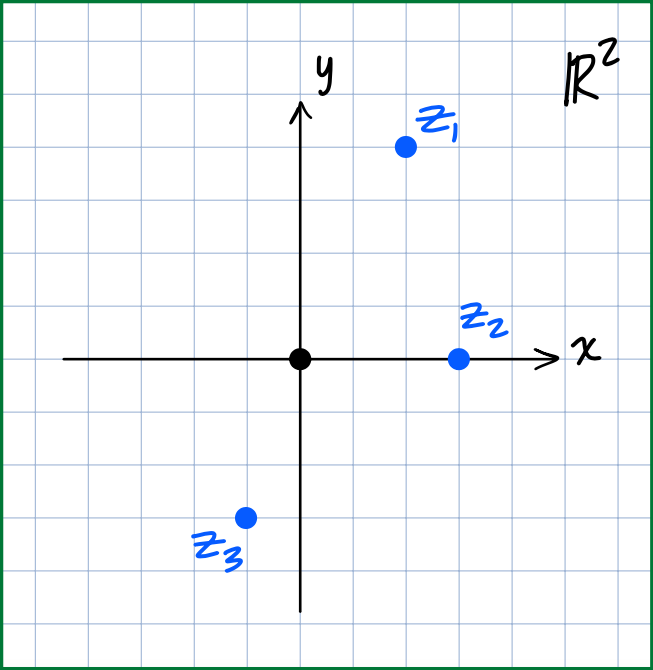
\includegraphics[width=0.3\linewidth]{complexplane}\hspace{4cm} 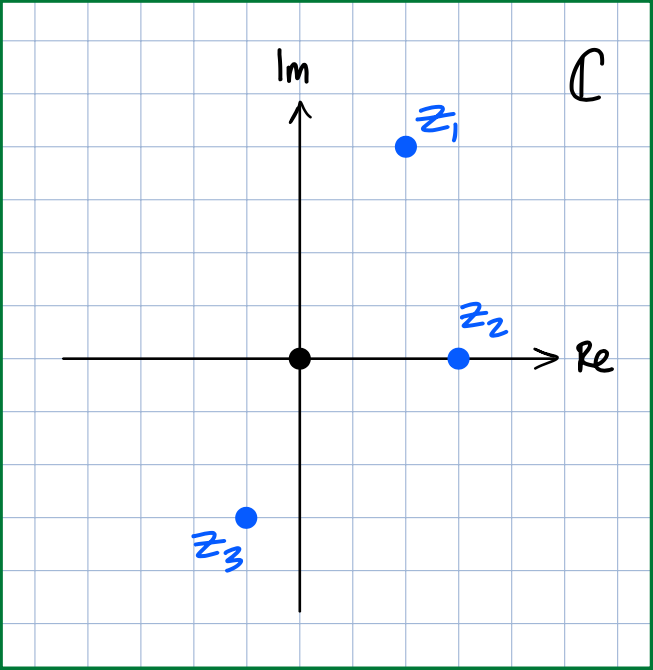
\includegraphics[width=0.3\linewidth]{complexplaneupdated}
\end{center}

\p Note that a point $z\in\COMPLEX$ lies on the $x$-axis if and only if it is real, and lies on the $y$-axis exactly when it is purely imaginary.  On the right, labels are updated accordingly.  $\COMPLEX = \REAL^{2}$ illustrated in this manner is referred to as the \DEF{complex plane}.
\vsp

\p A complex number $z = a + bi$ may also be geometrically represented as an arrow pointing from the origin to the point $(a,b)$ in $\REAL^{2}$, shown on the left.
\vsp

\begin{center}
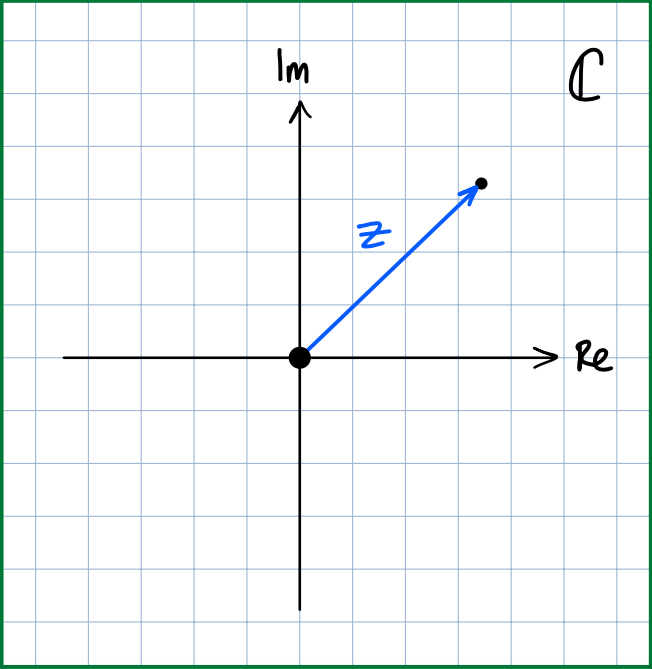
\includegraphics[width=0.3\linewidth]{geometriccomplex}\hspace{4cm} 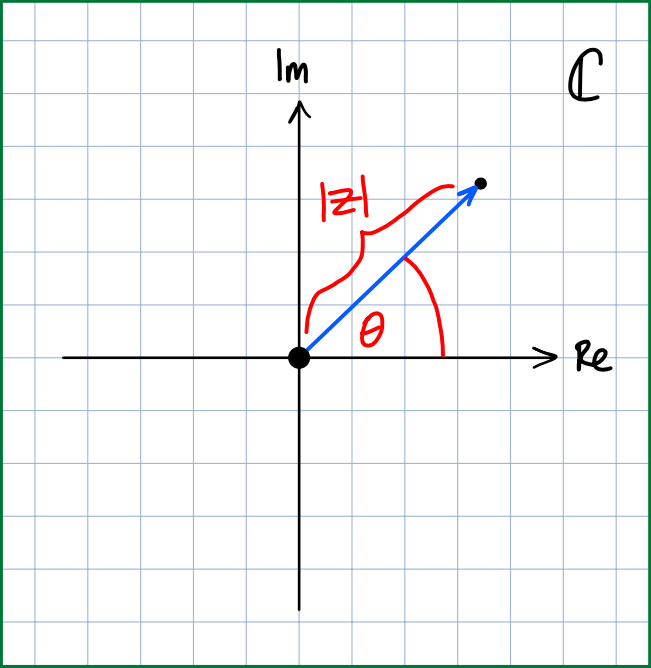
\includegraphics[width=0.3\linewidth]{geometriccomplexlabelled}
\end{center}

\p Any such arrow has length given by the complex modulus of $z$, and forms an angle $\theta$ of inclination, measured counter-clockwise from the positive half of the real axis, shown on the right.

\begin{definition}
An ordered pair $(r,\theta)$ is a polar coordinate representation of $z$ if $r = |z|$ and $\theta$ is the angle of inclination of $z$, measured counter-clockwise from the positive half of the real axis.  In this case $\theta$ is called an \DEF{argument} of $z$.
\end{definition}
%
\begin{examples}~
\begin{enumerate}[(a)]
\item $(2,0)$ is a polar coordinate representation of $2$.
\item $(1,\pi/2)$ is a polar coordinate representation of $i$.
\item $(3,-\pi/2)$ is a polar coordinate representation of $-3i$.
\end{enumerate}
\end{examples}
%
\begin{remarks}~
\begin{enumerate}[(1)]
\item Since arguments of complex numbers are not unique, neither are polar coordinate representations!  For example both $\pi$ and $3\pi$ are arguments of the real number $-1$, which therefore has both $(1,\pi)$ and $(1,3\pi)$ as polar coordinate representations.
\item If $(r,\theta)$ is a polar coordinate representation of a complex number $z$, the Pythagorean Theorem forces real and imaginary parts of $z$ to be given by
\begin{center}
$\RE{z} = r\cos(\theta)$ and $\IM{z} = r\sin(\theta)$.
\end{center}
It follows that $z = r\cos(\theta) + ir\sin(\theta) = r(\cos(\theta) + i\sin(\theta)) = re^{i\theta}$, which is referred to as the \DEF{polar form} of $z$.
\end{enumerate}
\end{remarks}
\newpage

\observation If $z_{1} = r_{1}e^{i\theta_{1}}$ and $z_{2} = r_{2}e^{i\theta_{2}}$ are written in polar form, then
\begin{center}
$\ds{z_{1}z_{2} = \left(r_{1}e^{i\theta_{1}}\right)\left(r_{2}e^{i\theta_{2}}\right) = (r_{1}r_{2})e^{i\theta_{1} + i\theta_{2}} = r_{1}r_{2}e^{i(\theta_{1} +\theta_{2})}}$
\end{center}
and
\begin{center}
$\ds{z_{1}/z_{2} = \frac{r_{1}e^{i\theta_{1}}}{r_{2}e^{i\theta_{2}}} = \left(\frac{r_{1}}{r_{2}}\right)e^{i\theta_{1} - i\theta_{2}} = \left(\frac{r_{1}}{r_{2}}\right)e^{i(\theta_{1} - \theta_{2})}}$.
\end{center}
\vsp

\p Consequently, to multiply complex numbers in polar form, we \emph{multiply their lengths and add their arguments}.  To divide them, we \emph{divide their lengths, and subtract their arguments}.  This is helpful to make use of when computing powers.  Indeed if $z = re^{i\theta}$ is in polar form and $n\geq 0$, then
\begin{center}
$z^{n} = \left(re^{i\theta}\right)^{n} = r^{n}\left(e^{i\theta}\right)^{n} = r^{n}e^{n(i\theta)} = r^{n}e^{i(n\theta)}$.
\end{center}
\vsp

\p Combining this with Euler's Formula in the special case when $r = 1$, we get the following.

\begin{theorem}[DeMoivre's Formula] $(\cos(\theta) + i\sin(\theta))^{n} = \cos(n\theta) + i\sin(n\theta)$
\end{theorem}

\begin{examples}~
\begin{enumerate}[(a)]
\item Let $z_{1} = 1 + i$ and $z_{2}  = \sqrt{3} - i$.  Find $z_{1}z_{2}$ and $z_{1}/z_{2}$ in polar form.
\item Find $(1 + i)^{16}$.
\end{enumerate}
\end{examples}
%
\begin{solution}
\begin{enumerate}[(a)]
\item Begin by writing $z_{1}$ and $z_{2}$ in polar form.  $z_{1}$ has modulus $\sqrt{2}$ and argument $\pi/4$, while $z_{2}$ has length $2$ and argument $-\pi/6$.  Hence we may write
\begin{center}
$z_{1} = \sqrt{2}e^{i(\pi/4)}$ and $z_{2} = 2e^{i(-\pi/6)}$
\end{center}
and compute
\begin{center}
$\ds{z_{1}z_{2} = \big(\sqrt{2}e^{i(\pi/4)}\big)\big(2e^{i(-\pi/6)}\big) = 2\sqrt{2}e^{i(\pi/4-\pi/6)} = 2\sqrt{2}e^{i(\pi/12)}}$
\end{center}
and
\begin{center}
$\ds{z_{1}/z_{2} = \frac{\sqrt{2}e^{i(\pi/4)}}{2e^{i(-\pi/6)}} = \left(\dfrac{\sqrt{2}}{2}\right)e^{i(\pi/4+\pi/6)} = \dfrac{\sqrt{2}}{2}e^{i(5\pi/12)}}$.
\end{center}
\item $(1+i)^{16} = \left(\sqrt{2}e^{i(\pi/4)}\right)^{16} = (\sqrt{2})^16\left(e^{i(\pi/4)}\right)^{16} = 2^{8}e^{16i(\pi/4)} = 256{\color{blue}\underbrace{{\color{black}e^{i(4\pi)}}}_{=1}} = 256$.
\end{enumerate}
\end{solution}
%
\begin{exercise}
Prove that for any $z\in\C$, $|z^{n}| = |z|^{n}$.
\end{exercise}
%
\subsection{Arguments}

\p Remember that the argument of a complex number is not unique!  For example, both $\pi/4$ and $9\pi/4$ are arguments for $1 + i$.  More generally, if $\theta$ is an argument for $z\in\COMPLEX$, then so is $\theta + 2\pi k$ for any $k\in \INTEGER$.
\vsp

\notation For any $z\in\COMPLEX$ with argument $\theta$, we may capture all of its arguments with the notation
\begin{center}
$\ARG{z} = \theta + 2\pi k$
\end{center}
where it is understood that $k$ varies over the set of integers.
\vsp

\fact For any $\theta\in\REAL$, there exists a unique $k^{\star}\in\INTEGER$ such that $\theta + 2\pi k^{\star}\in (-\pi, \pi]$.  In this case $\theta + 2\pi k^{\star}$ is called the \DEF{principle argument} of $z$, and is denoted by $\PARG{z}$.
\vsp

\begin{examples}~
\begin{enumerate}[(a)]
\item For $z = 1 + i$, $\ARG{z} = \pi/4 + 2\pi k$, and $\PARG{z} = \pi/4$.
\item $\PARG{e^{i(5\pi/3)}} = -2\pi/3$.
\end{enumerate}
\end{examples}

\begin{exercise}
Is it true that $\PARG{z_1z_2} = \PARG{z_1} + \PARG{z_2}$ for every $z_{1},z_{2}\in\C$?
\end{exercise}

\subsection{Roots of Complex Numbers}\label{rootsofunitysection}

\p For the duration of this section, $n$ shall always denote a positive integer.
%
\begin{definition}
A complex number $z$ is said to be an \DEF{$n$th root of unity} if $z^{n} = 1$.
\end{definition}

\begin{example}
The fourth roots of unity are the complex numbers $1, -1, i$, and $-i$.  Since they each have modulus $1$, they all lie on the unit circle (shown below on the left).
\end{example}
%
\begin{center}
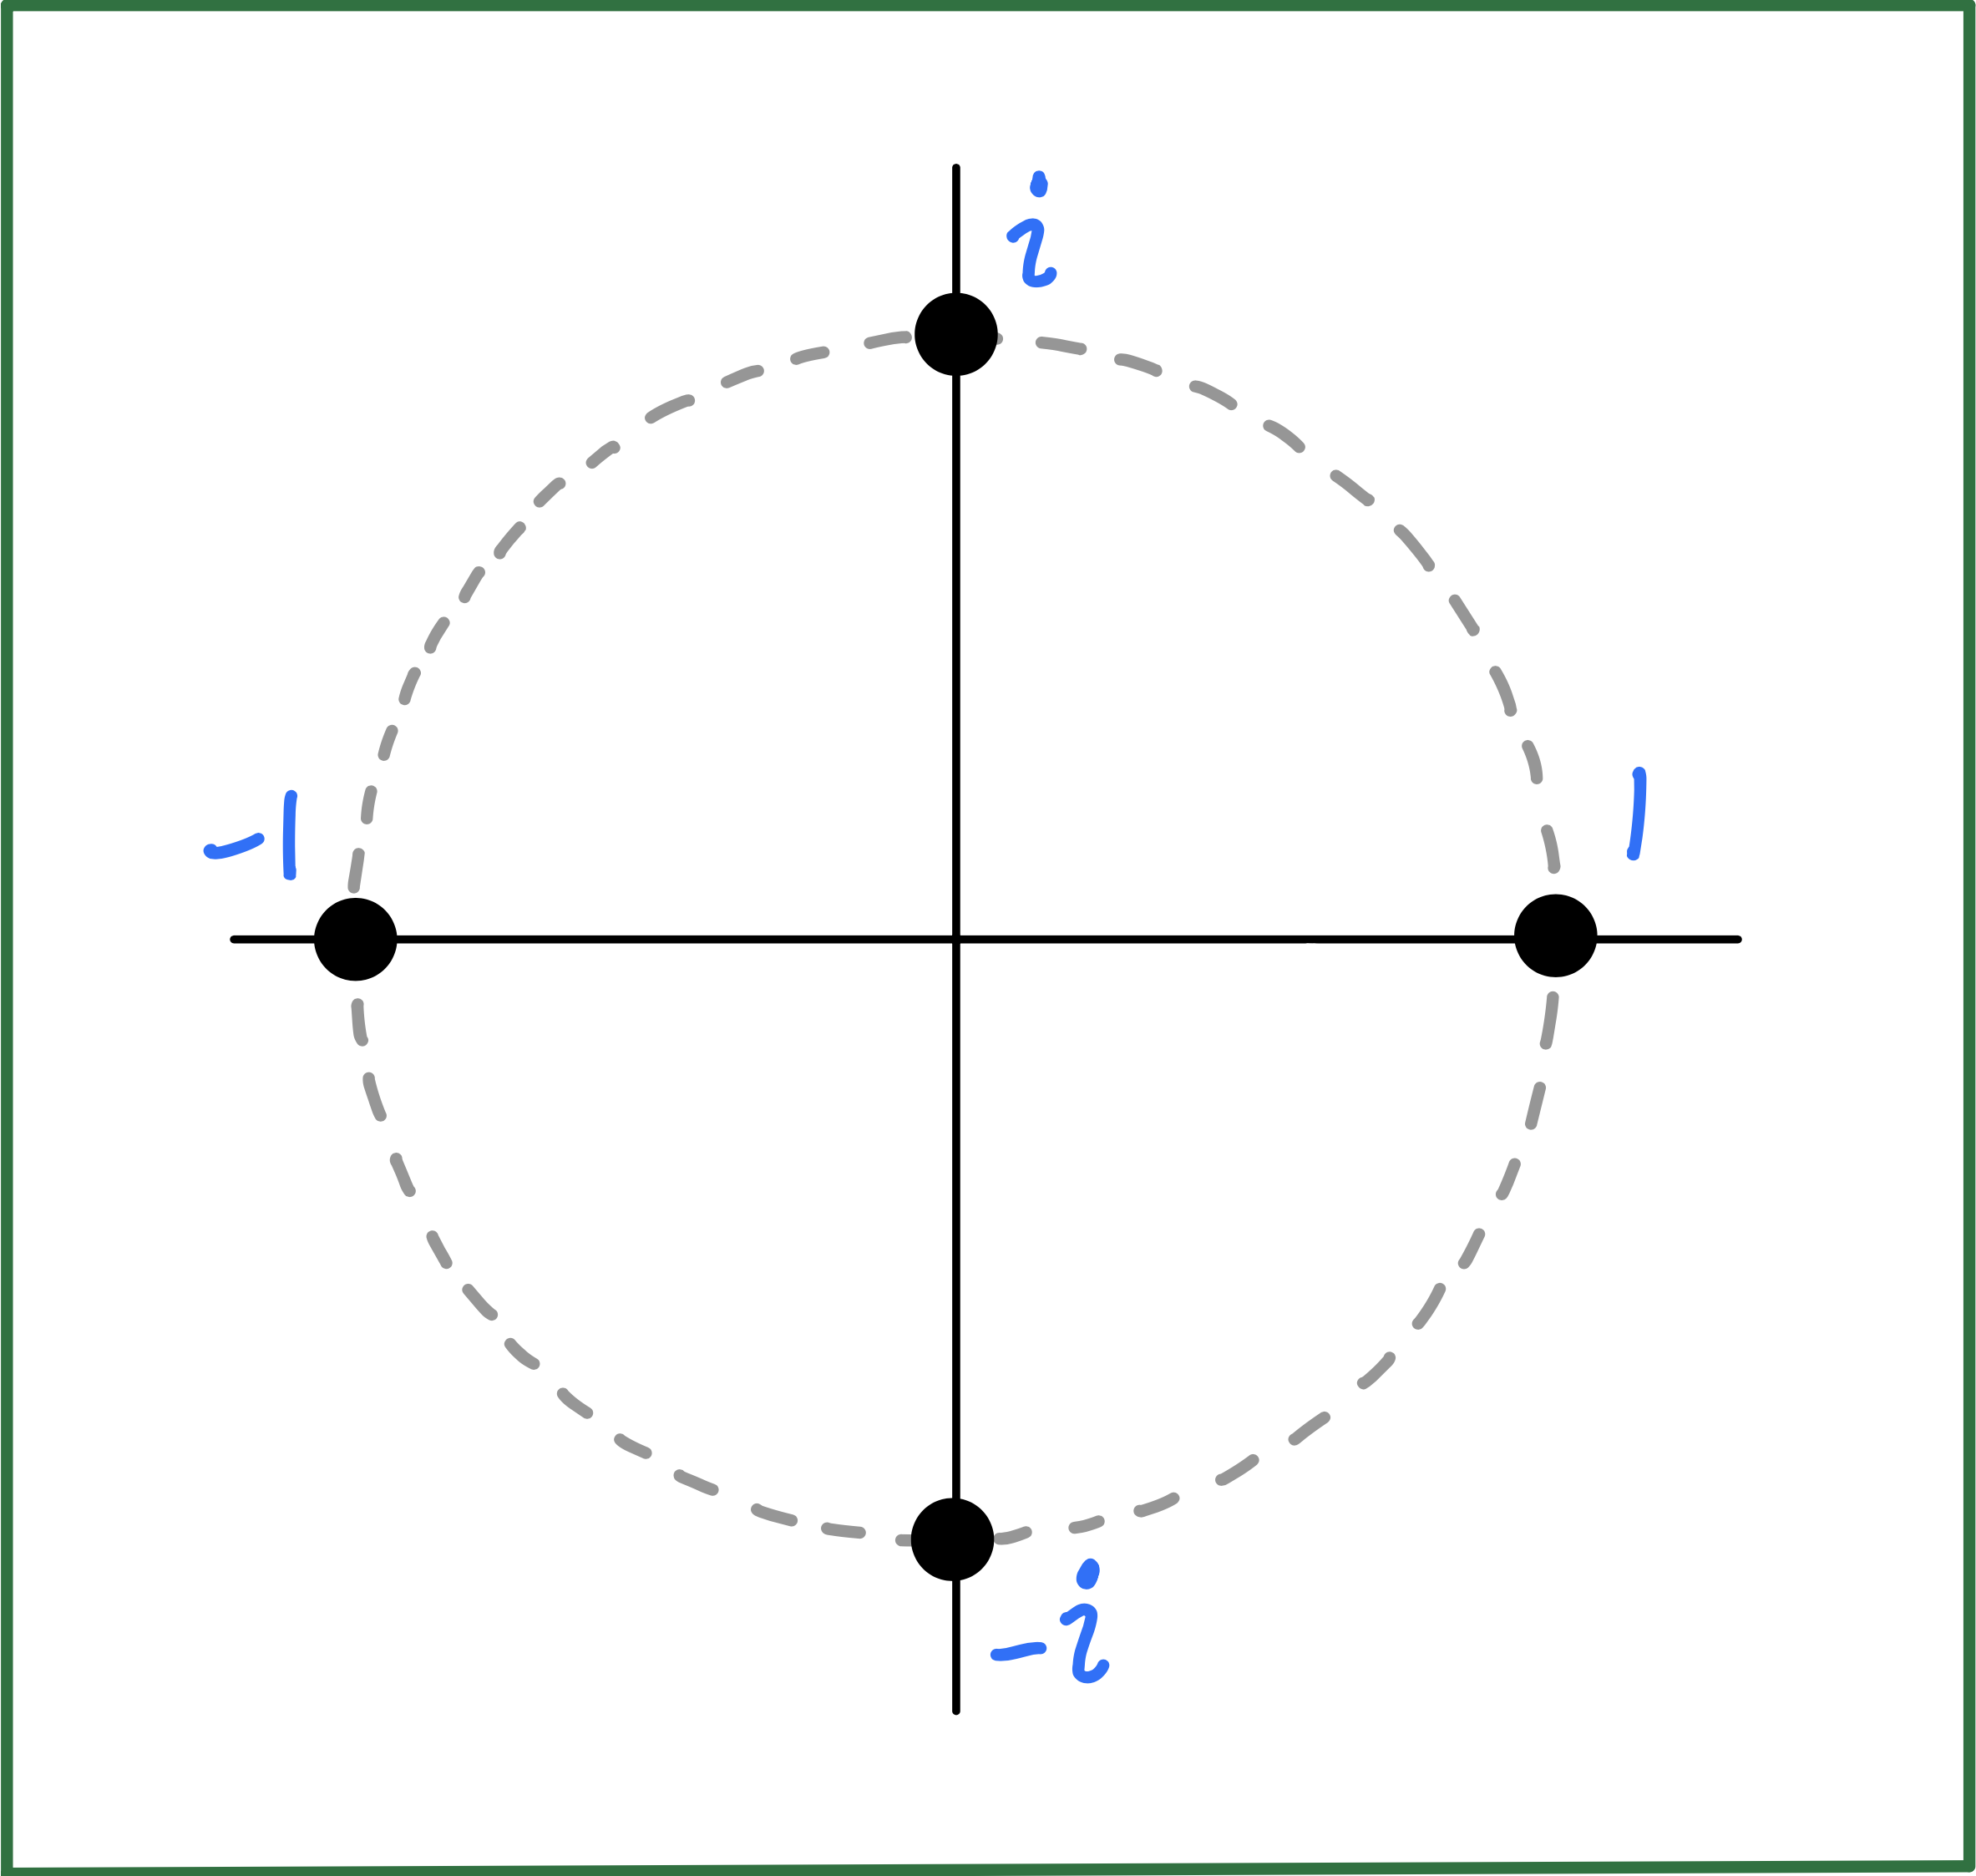
\includegraphics[width=0.3\linewidth]{4throotsofunity}\hspace{4cm} 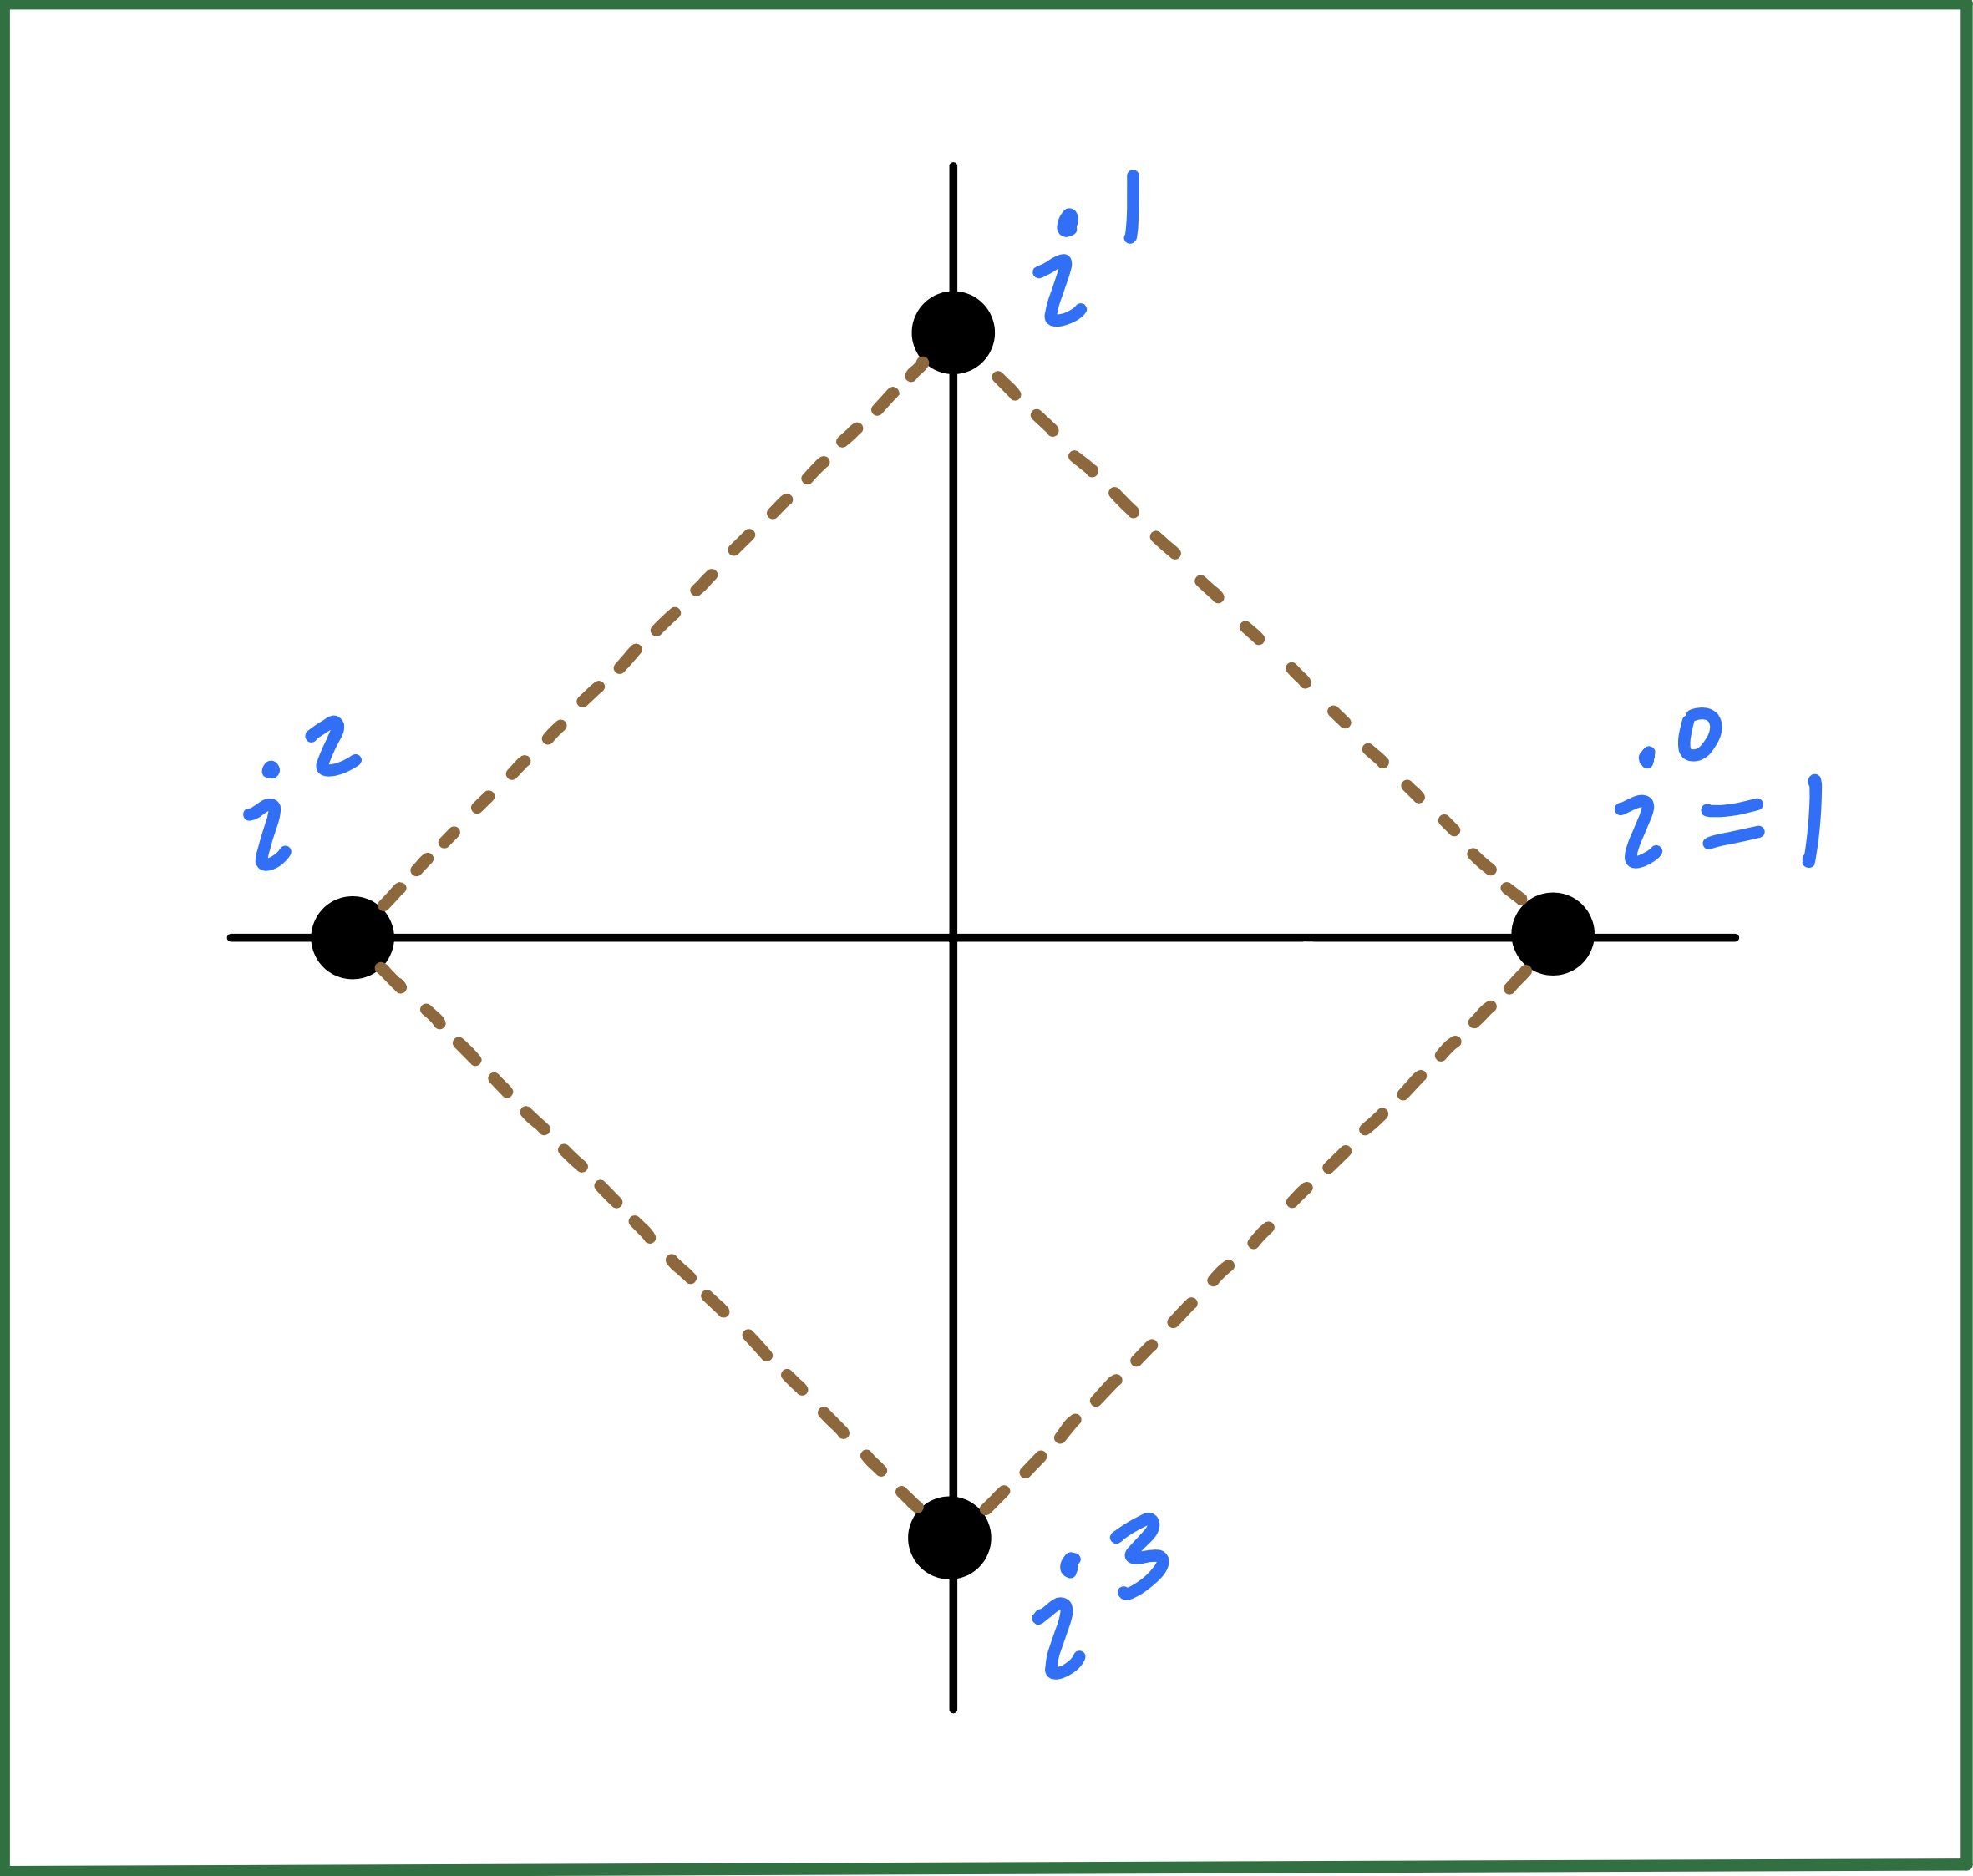
\includegraphics[width=0.3\linewidth]{powersofi}
\end{center}
\vsmsp

\p Note also that the fourth roots of unity are all powers of $i = e^{i(\pi/2)} = e^{2\pi i/4}$, forming the vertices of a square centered at the origin (shown above on the right).
\vsp 

\GRAYLINE
\vsmsp

\p To classify the general $n$th roots of unity, first note that $\omega = e^{2\pi i/n}$ is an $n$th root of unity, since
\begin{center}
$\omega^{n} = \left(e^{2\pi i/n}\right)^{n} = e^{n[i(2\pi/n)]} = e^{i(2\pi)} = 1$.
\end{center}
\vsp

\p Next, observe that for any $k\in \Z$, $\omega^{k}$ is also an $n$th root of unity, since
\begin{center}
$\left(\omega^{k}\right)^{n} = \left(\omega^{n}\right)^{k} = 1^{k} = 1$.
\end{center}

\p And in fact, the powers of $\omega$ account for \emph{all} of the $n$th roots of unity.  To see why this is the case, suppose $z = re^{i\theta}\in\C$ is chosen so that $z^n = r^ne^{i(n\theta)} = 1$.  By considering the polar form of $1$, it may be seen that $r^{n} = 1$ and $n\theta = 2\pi k$ for some $k\in\INTEGER$.  It follows that $r = 1$ and $\theta = 2\pi k/n$ for some $k\in\INTEGER$.  Therefore $z = e^{i(2\pi k/n)} = \omega^{k}$. 
\vsp

\p Finally, note that sequential powers of $\omega$ eventually repeat, since $\omega^{k+n} = \omega^{k}{\color{blue}\underbrace{\color{black}\omega^{n}}_{=1}} = \omega^{k}$ for any $k\in\Z$.
%
\begin{theorem}\label{rootsofunityclassification}
The $n$ distinct $n$th roots of unity are given by $\omega^{k} = e^{2\pi i k/n}$, with $k\in\INTEGER$ with $0\leq k < n$, where
\begin{center}
$\omega = e^{2\pi i/n}$.
\end{center}
\end{theorem}


\begin{example}\label{fifthrootsunityexample}
Find all of the fifth roots of unity.
\end{example}
%
\begin{solution}
Set $\omega = e^{i(2\pi/5)}$.  By the foregoing, the fifth roots of unity are given by
\begin{center}
$\omega^{0}, \omega^{1}, \omega^{2},\omega^{3}$ and $\omega^{4}$,
\end{center}
which when worked out using Euler's Formula are
\begin{itemize}[\ ]
\item $\omega^{0} = 1$,
\item $\omega^{1} = e^{i(2\pi/5)} = \cos(2\pi/5) + i\sin(2\pi/5)$,
\item $\omega^{2} = e^{i(4\pi/5)} = \cos(4\pi/5) + i\sin(4\pi/5)$,
\item $\omega^{3} = e^{i(6\pi/5)} = \cos(6\pi/5) + i\sin(6\pi/5)$, and
\item $\omega^{4} = e^{i(8\pi/5)} = \cos(8\pi/5) + i\sin(8\pi/5)$.
\end{itemize}
\end{solution}
\vsp

\p The fifth roots of unity $\omega^{0}, \omega^{1}, \omega^{2},\omega^{3}$ and $\omega^{4}$ from Example \ref{fifthrootsunityexample} are sketched below on the left.  Note that they form the vertices of a regular hexagon with center of mass located at the origin, which is shown on the right.

\begin{center}
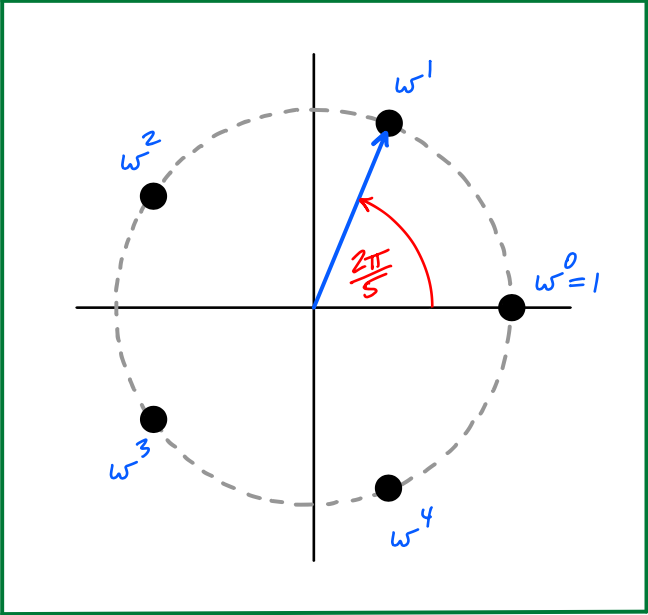
\includegraphics[width=0.3\linewidth]{fifthrootsunity}\hspace{4cm} 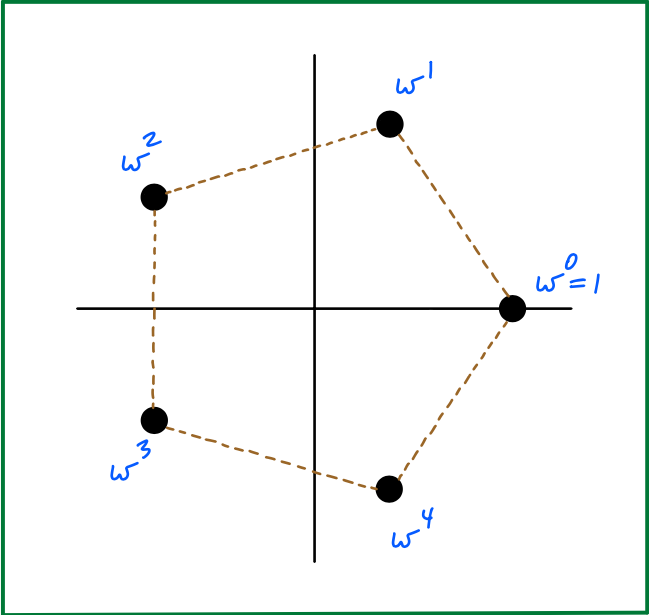
\includegraphics[width=0.3\linewidth]{fifthrootsunityhexagon}
\end{center}
%
\begin{definition} Let $n> 1$.  A complex number $\omega\in\COMPLEX$ is a \DEF{primitive $n$th root of unity} if $\omega^{n} = 1$ and $\omega^{k}\neq 1$ whenever $0 < k < n$.
\end{definition}
%
\begin{examples}~
\begin{enumerate}[(a)]
\item $i$ is a primitive $4$th root of unity, since $i^{4} = 1$ but $i^{1} = i\neq 1$, $i^{2} = -1\neq 1$, and $i^3 = -i\neq 1$.
\item $-1$ is not a primitive $4$th root of unity, since $(-1)^2 = 1$.
\end{enumerate}
\end{examples}
\vsmsp

%
\note $e^{i(2\pi/n)}$ is a primitive $n$th root of unity -- but not the only one!
\vsmsp

\begin{lemma}\label{primitiverootlemma}
Let $k\in\Z$ and $\omega = e^{i(2\pi/n)}$.  $\omega^{k} = 1$ if and only if $n|k$.
\end{lemma}
%
\begin{proof}
By the Division algorithm, choose $q,r\in\Z$ such that $k = qn + r$ and $0\leq r < n$.  Then
\begin{center}
$\omega^{k} = \omega^{qn + r} = \omega^{qn}\omega^{r} = \big(\omega^{n})^{q}\omega^{r} = 1^{q}\omega^{r} = \big(e^{i(2\pi/n)}\big)^{r} = e^{i(2\pi r/n)}$,
\end{center}
which equals $1$ if and only if $r/n\in\Z$.
\end{proof}
%
\begin{theorem}
If $\omega = e^{i(2\pi/n)}$ and $k\geq 1$ is an integer, then
\begin{center}
$z = \omega^{k} = \big(e^{i(2\pi n)}\big)^{k} = e^{i(2\pi k/n)}$
\end{center}
is a primitive $n$th root of unity if and only if $\GCD{n,k} = 1$.
\end{theorem}
%
\begin{proof}~

$(\Rightarrow)$ Suppose $\GCD{n,k} = d > 1$.  Then we may write $k = md$ for some $m\in\Z$.  Then $n/d < n$ and
\begin{center}
$z^{n/d} = \big(\omega^{k}\big)^{n/d} = \big(\omega^{md}\big)^{n/d} =  \big(\omega^{m}\big)^{d(n/d)} = \big(\omega^{m}\big)^{n} = \big(\omega^{n}\big)^{m} = 1^{m} = 1$,
\end{center}
which shows that $z$ is not a primitive $n$th root of unity.
\vsp

$(\Leftarrow)$ Assume $\GCD{n,k} = 1$ and suppose for a contradiction that $z^{d} = 1$ for some $d\in\Z$ with $0 < d < n$.  Then
\begin{center}
$1 = z^{d} = \big(e^{i(2\pi k/n)}\big)^{d} = \big(e^{i(2\pi/n)}\big)^{kd}$.
\end{center}
By Lemma \ref{primitiverootlemma}, $kd/n$ must be an integer.  Since $n$ and $k$ are co-prime, Corollary \ref{dividesproductonefactorcoprime} forces $n|d$.  This contradicts the fact that $d<n$.
\end{proof}
%
\begin{definition}
Let $z = re^{i\theta}\in \C$ and $n\geq 1$ be an integer. The \DEF{complex $n$th roots} of $z$ are given by
\begin{center}
$z^{1/n} := \sqrt[n]{r}e^{i(\theta + 2\pi k)/n}$, where $k\in\SET{0, 1, \ldots, n -1}$.
\end{center}
\end{definition}
%
\begin{example}
Find all of the cube roots of $\sqrt{2} + i\sqrt{2}$.
\end{example}
%
\begin{solution}
Letting $z = \sqrt{2} + i\sqrt{2}$, we see that $|z| = 2$ and that $r = \pi/4$ is an argument of $z$.  Hence its polar form is given by
\begin{center}
$z = 2e^{i(\pi/4)}$.
\end{center}
\p It follows that
\begin{center}
$z^{1/3} = \sqrt[3]{2}e^{i(\pi/4 + 2\pi k)/3}$, where $k = 0,1,2$,
\end{center}
\p and hence
\begin{itemize}[\ ]
\item $\sqrt[3]{2}e^{i(\pi/4)/3} = \sqrt[3]{2}e^{i(\pi/12)} = \sqrt[3]{2}\cos(\pi/12) + i\sqrt[3]{2}\sin(\pi/12)$,
\item $\sqrt[3]{2}e^{i(\pi/4 + 2\pi)/3} = \sqrt[3]{2}e^{i(3\pi/4)} = \sqrt[3]{2}\cos(3\pi/4) + i\sqrt[3]{2}\sin(3\pi/4)$, and
\item $\sqrt[3]{2}e^{i(\pi/4 + 4\pi)/3} = \sqrt[3]{2}e^{i(17\pi/12)} = \sqrt[3]{2}\cos(17\pi/12) + i\sqrt[3]{2}\sin(17\pi/12)$
\end{itemize}
are the cube roots of $\sqrt{2} + i\sqrt{2}$.
\end{solution}
%
\begin{remark}
When seeking the $n$th roots of a complex number $z$, an alternative approach is as follows.  Find \emph{any} $n$th root of $z$ and multiply it by each of the $n$th roots of unity.
\end{remark}
%
\begin{example}
Find all the fifth roots of $2$.
\end{example}
%
\begin{solution}
The real number $\sqrt[5]{2}$ is a fifth root of $2$.  To find the others, multiply it by the various powers of $\omega = e^{2\pi i/5}$ to obtain a complete list of the fifth roots of $2$:
\begin{itemize}[\ ]
\item $\sqrt[5]{2}\omega^{0} = \sqrt[5]{2}$
\item $\sqrt[5]{2}\omega^{1} = \sqrt[5]{2}e^{2\pi i/5} = \sqrt[5]{2}\cos(2\pi/5) + i\sqrt[5]{2}\sin(2\pi/5)$
\item $\sqrt[5]{2}\omega^{2} = \sqrt[5]{2}e^{4\pi i/5} = \sqrt[5]{2}\cos(4\pi/5) + i\sqrt[5]{2}\sin(4\pi/5)$
\item $\sqrt[5]{2}\omega^{3} = \sqrt[5]{2}e^{6\pi i/5} = \sqrt[5]{2}\cos(6\pi/5) + i\sqrt[5]{2}\sin(6\pi/5)$
\item $\sqrt[5]{2}\omega^{4} = \sqrt[5]{2}e^{8\pi i/5} = \sqrt[5]{2}\cos(8\pi/5) + i\sqrt[5]{2}\sin(8\pi/5)$
\end{itemize}
\end{solution}
%
\section{Congruence in \texorpdfstring{$\INTEGER$}{Z} and Modular Arithmetic}\label{congruencechapter}

\subsection{Congruence and Congruence Classes}

\begin{definition}\label{congruenceoperations}
Let $a,b,n\in\INTEGER$ with $n > 0$.  We say that $a$ is \DEF{congruent to $b$ modulo $n$} if $n|b-a$.
\end{definition}

\notation In this case we write $a\equiv b$ (mod $n$), or $a\overset{n}{\equiv}b$.  Otherwise we write $a\not\equiv b$ (mod $n$), or $a\not\overset{n}{\equiv}b$.

\example $9\overset{2}{\equiv}5$ and $9\overset{4}\equiv{5}$ but $9\not\overset{2}{\equiv}5$.

\begin{theorem}\label{congruenceproperties}Let $n\in\INTEGER$ with $n > 0$.
\begin{enumerate}[(1)]
\item $a\overset{n}{\equiv} a$ for any $a\in\INTEGER$.
\item If $a,b\in\INTEGER$ such that $a\overset{n}{\equiv} b$, then $b\overset{n}{\equiv} a$.
\item If $a,b,c\in\INTEGER$ such that $a\overset{n}{\equiv} b$ and $b\overset{n}{\equiv} c$, then $a\overset{n}{\equiv} c$.
\end{enumerate}
\end{theorem}
%
\begin{proof}~
\begin{enumerate}[(1)]
\item For any $a\in\INTEGER$, we have $n|a-a$, since $a-a = 0$.  Hence $a\overset{n}{\equiv} a$.
\item For any $a,b\in\INTEGER$, if $a\overset{n}{\equiv} b$, then $n|b-a$.  Hence $n|a-b$, so $b\overset{n}{\equiv} a$.
\item For any $a,b,c\in\INTEGER$, if $a\overset{n}{\equiv} b$ and $b\overset{n}{\equiv} c$, then $n$ divides both $b-a$ and $c-b$.  It follows that $n$ also divides $c-a = (c-b) + (b-a)$.  Hence $a\overset{n}{\equiv} c$.\hfill \qedhere
\end{enumerate}
\end{proof}
%
\begin{theorem}\label{congruencereplacement}
If $a,b,c,d\in\INTEGER$ such that $a\overset{n}{\equiv} b$ and $c\overset{n}{\equiv} d$, then $a + c\overset{n}{\equiv} b + d$ and $ac\overset{n}{\equiv} bd$.
\end{theorem}
%
\begin{proof}
By assumption, $n|b-a$ and $n|d-c$.  It follows that
\begin{center}
$(b+d) - (a+c) = (b-a) + (d-c)$
\end{center}
and
\begin{center}
$bd - ac = bd - ad + ad - ac = d(b-a) + a(d-c)$.
\end{center}
are both divisible by $n$.  Hence $a + c\overset{n}{\equiv} b + d$ and $ac\overset{n}{\equiv} bd$.
\end{proof}
\vsp

\p In particular, if $a,b\in\INTEGER$ such that $a\overset{n}{\equiv} b$, then for any $c\in\INTEGER$, $a + c\overset{n}{\equiv} b + c$ and $ac\overset{n}{\equiv} bc$ for any $c\in\INTEGER$.

\begin{example}
Find all solutions to the congruence $2x\overset{5}{\equiv} 3$.
\end{example}

\solution Every integer $x$ is congruent modulo $5$ to exactly one element of the set $\SET{0,1,2,3,4}$.  So check each possibility:
\begin{itemize}[\ ]
\item If $x\overset{5}{\equiv}0$, then $2x\overset{5}{\equiv} 2\cdot 0 = 0\not\overset{5}{\equiv}2$.
\item If $x\overset{5}{\equiv}1$, then $2x\overset{7}{\equiv}2\cdot 1 = 2\overset{5}{\equiv}2$.
\item If $x\overset{5}{\equiv}2$, then $2x\overset{7}{\equiv}2\cdot 2 = 4\not\overset{5}{\equiv}2$.
\item If $x\overset{5}{\equiv}3$, then $2x\overset{7}{\equiv}2\cdot 3 = 6\not\overset{5}{\equiv}2$.
\item If $x\overset{5}{\equiv}4$, then $2x\overset{7}{\equiv}2\cdot 4 = 8\not\overset{5}{\equiv}2$.
\end{itemize}
Hence $2x\overset{5}{\equiv} 3$ is satisfied exactly when $x\overset{5}{\equiv}1$.
\vsp

\begin{exercises} \phantom{ }
\begin{enumerate}[(1)]
\item Find all solutions to the congruence $3x\overset{7}{\equiv} 4$.
\item Which of the following congruences have solutions?
\begin{enumerate}[(a)]
\item $x^{2}\overset{3}{\equiv} 1$
\item $x^{2}\overset{7}{\equiv} 2$
\item $x^{2}\overset{11}{\equiv} 3$
\end{enumerate}
\item Let $a,b,n\in\INTEGER$ with $n > 0$.  Prove that if $a\overset{n}{\equiv}b$, then $a^2 + b^2\overset{n^2}{\equiv}2ab$.
\item Suppose $a,b\in\INTEGER$ such that $a\overset{p}{\equiv}b$ for every prime $p$.  Prove that $a = b$.
\end{enumerate}
\end{exercises}
%
\begin{definition}\label{congruenceclassmodndefn}
Let $a,n\in\INTEGER$ with $n > 0$.  The \DEF{congruence class of $a$ modulo $n$} is defined by
\begin{center}
$[a] = \SET{b\in\INTEGER : a\overset{n}{\equiv}b} = \SET{a + kn:k\in\INTEGER}$.
\end{center}
\end{definition}
%
\begin{example}
If $n = 5$, then
\begin{itemize}[\ ]
\item $[0] = \SET{0 + 5k:k\in\INTEGER} = \SET{5k:k\in\INTEGER}$
\item $[1] = \SET{1 + 5k:k\in\INTEGER} = \SET{1 + 5k:k\in\INTEGER}$
\item $[2] = \SET{2 + 5k:k\in\INTEGER} = \SET{2 + 5k:k\in\INTEGER}$
\item $[3] = \SET{3 + 5k:k\in\INTEGER} = \SET{3 + 5k:k\in\INTEGER}$
\item $[4] = \SET{4 + 5k:k\in\INTEGER} = \SET{4 + 5k:k\in\INTEGER}$
\item $[5] = \SET{5 + 5k:k\in\INTEGER} = \SET{5(1 + k):k\in\INTEGER} = \SET{5k:k\in\INTEGER} = [0]$
\end{itemize}
\p In a similar fashion, $[6] = [1]$ and $[7] = [2]$, etc.
\end{example}
%
\begin{theorem}\label{congruenceequalitycriterion}
Let $a,b,n\in\INTEGER$ with $n > 0$.  $a\overset{n}{\equiv}b$ if and only if $[a] = [b]$.
\end{theorem}
%
\begin{proof}
$(\Rightarrow)$ It must be verified that if $a\overset{n}{\equiv}b$, then $[a] = [b]$.

$(\subset)$ Suppose $c\in[a]$.  Then $c\overset{n}{\equiv}a$.  By assumption, $a\overset{n}{\equiv}b$.  Hence by Theorem \ref{congruenceproperties} (3), we must have $c\overset{n}{\equiv}b$, i.e, $c\in[b]$.

$(\supset)$ This direction follows from an identical argument.

$(\Leftarrow)$ Suppose $[a] = [b]$.  By Theorem \ref{congruenceproperties}, $a\overset{n}{\equiv}a$ and hence $a\in [a]$.  It follows that $a\in[b]$ and therefore $a\overset{n}{\equiv}b$, as required.
\end{proof}
%
\begin{corollary}\label{disjointorsame}
For any $a,b,n\in\INTEGER$ with $n > 0$, either $[a] = [b]$ or $[a]\cap [b] = \emptyset$.
\end{corollary}
%
\begin{proof}
Suppose $a,b\in\INTEGER$ with $[a]\cap[b]\neq\emptyset$.  Then choose $c\in[a]\cap[b]$.  It follows that $a\overset{n}{\equiv}c$ and $b\overset{n}{\equiv}c$.  Therefore $a\overset{n}{\equiv}c\overset{n}{\equiv}b$.  By Theorem \ref{congruenceequalitycriterion}, it follows that $[a] = [b]$.
\end{proof}
%
\begin{corollary}\label{elementsofZn}
Let $n\in\INTEGER$ with $n>0$.
\begin{enumerate}[(1)]
\item If $a\in\INTEGER$ and $r$ is the remainder when $a$ is divided by $n$, then $[a] = [r]$.
\item There are exactly $n$ distinct congruence classes modulo $n$, namely $[0], [1], [2],\ldots, [n-1]$.
\end{enumerate}
\end{corollary}
%
\begin{proof}~
\begin{enumerate}[(1)]
\item Use the Division algorithm to write $a = nq + r$ for some $r,n\in\INTEGER$ with $0\leq r < n$.  Since $a - r = nq$, $n|a-r$ and hence $a\overset{n}{\equiv}r$.  Therefore $[a] = [r]$ by Theorem \ref{congruenceequalitycriterion}.
\item First, note that $[0], [1], [2],\ldots, [n-1]$ are all distinct congruence classes.  Indeed if $[i] = [j]$ for some $i,j\in\INTEGER$ with $0\leq i,j < n$, then $i\overset{n}{\equiv}j$ and hence $n|i-j$.  By the way $i$ and $j$ were chosen, we must have $-n+1 < i-j < n-1$.  Since $i-j$ is divisible by $n$, we must have $i-j = 0$, or equivalently, $i=j$.  On the other hand if $a\in\INTEGER$, then by (1) $[a] = [r]$, where $r$ is the remainder of $a$ when divided by $n$.  Since $0\leq r < n-1$, this completes the proof.\qedhere
\end{enumerate}
\end{proof}
%
\begin{definition}
$\ZN$ is the set of all congruence classes modulo $n$.  That is, $\ZN = \SET{[0], [1], [2],\ldots, [n-1]}$.
\end{definition}
%
\begin{exercises}~
\begin{enumerate}
\item Decide whether each of the following statements are true.  If they are true, then prove them.  Otherwise, provide a counter-example.
\begin{enumerate}[(a)]
\item If $a^2\overset{n}{\equiv}b^2$, then either $a\overset{n}{\equiv}b$ or $a\overset{n}{\equiv}-b$.
\item If $p$ is prime and $a^2\overset{p}{\equiv}b^2$, then either $a\overset{p}{\equiv}b$ or $a\overset{p}{\equiv}-b$.
\item If $[a] = [b]$ in $\ZN$, then $\GCD{a,n} = \GCD{b,n}$.
\end{enumerate}
\item If $[a] = [1]$ in $\ZN$, prove that $\GCD{a,n} = 1$.  Demonstrate also that the converse fails to be true in general.
\end{enumerate}
\end{exercises}
%
\subsection{Modular Arithmetic}
\begin{definition}
The \DEF{sum} and \DEF{product} of $[a]$ and $[b]$ in $\ZN$ are given by
\begin{center}
$[a]\oplus [b] = [a + b]$ and $[a]\odot[b] = [ab]$.
\end{center}
\end{definition}
%
\p Note that in order for these operations to be well-defined, it must be the case that the sum and product of two congruence classes do not depend on the representative chosen from the two congruence classes being added or multiplied.  That is, if $[a] = [a']$ and $[b] = [b']$, then $[a+b] = [a' + b']$ and $[ab] = [a'b']$.
\smsp

\p But this is equivalent to the requirement that $a + b\overset{n}{\equiv} a' + b'$ and $ab\overset{n}{\equiv} a'b'$ whenever $a\overset{n}{\equiv} a'$ and $b\overset{n}{\equiv}b'$.  And this follows immediately from Theorem \ref{congruencereplacement}.
%
\begin{example}In $\Z_{5}$, the addition and multiplication tables are shown below.
\vsmsp

\begin{center}
\bgroup
\def\arraystretch{1.5}
\begin{tabular}{c|ccccc}
$\oplus$ & [0] & [1] & [2] & [3] & [4]\\
\hline
$[0]$ & [0] & [1] & [2] & [3] & [4]\\
$[1]$ & [1] & [2] & [3] & [4] & [0]\\
$[2]$ & [2] & [3] & [4] & [0] & [1]\\
$[3]$ & [3] & [4] & [0] & [1] & [2]\\
$[4]$ & [4] & [0] & [1] & [2] & [3]
\end{tabular}
\hspace{3cm}
\begin{tabular}{c|ccccc}
$\odot$ & [0] & [1] & [2] & [3] & [4]\\
\hline
$[0]$ & [0] & [0] & [0] & [0] & [0]\\
$[1]$ & [0] & [1] & [2] & [3] & [4]\\
$[2]$ & [0] & [2] & [4] & [1] & [3]\\
$[3]$ & [0] & [3] & [1] & [4] & [2]\\
$[4]$ & [0] & [4] & [3] & [2] & [1]
\end{tabular}
\egroup
\end{center}
\end{example}
%
\exercise Write out the addition and multiplication tables for $\Z_6$.
\vsp
%
\begin{definition}
A \DEF{relation} on a set $A$ is a subset of $A\times A$.
\end{definition}
\vsp

\notation If $T$ is a relation on a set $A$, and $a,b\in A$ are such that $(a,b)\in T$, then we write $a\sim b$.
\vsp

\begin{definition}
A relation $T$ on a set $A$ is said to be an \DEF{equivalence relation} if the following conditions are met:
\begin{enumerate}[(1)]
\item $a\sim a$, for all $a,\in A$.
\item $a\sim b \Rightarrow b\sim a$, for all $a,b\in A$.
\item $a\sim b$ and $b\sim c \Rightarrow a\sim c$, for all $a,b,c\in A$.
\end{enumerate}
\end{definition}
%
\begin{examples}\label{equivalencerelationexamples}~
\begin{enumerate}[(a)]
\item Define the relation $T$ on $\REAL$ by $T = \SET{(x,x):x\in\REAL}\cup \SET{(x,-x):x\in\REAL}$.  Then $(x,y)\in T$ exactly when $x = y$ or $x = -y$.  That is, $x\sim y$ if and only if $|x| = |y|$.
\item $S = \SET{\Big((x,y), (w,z)\Big):x,y,w,z\in\REAL\text{ with }x = w}$ is a relation on $\REAL^{2}$.  In this case, $(x,y)\sim (w,z)$ if and only if $x = w$.
\item Define another relation on $\REAL^{2}$ by $(x,y)\sim (w,z)$ if and only if both $(x,y)$ and $(w,z)$ are the same distance from the origin.
\item Let $A$ be the set of all students in this class.  Define a relation on $A$ by imposing $a\sim b$ whenever $a$ and $b$ were born in the same month.
\item Let $n\in \INTEGER$ with $n > 0$ and define the relation $T = \SET{(a,b):n|b-a}$.  In other words, $a\sim b$ if and only if $a\overset{n}{\equiv}b$.  By Theorem \ref{congruenceproperties}, $T$ is an equivalence relation.  For this reason, equivalence relations may be thought of as a generalization of congruence modulo $n$.
\end{enumerate}
\end{examples}
%
%\begin{definition}
%A partition of a set $A$ is a collection $\mathcal{T}$ of subsets of $A$ with the properties:
%\begin{enumerate}[(1)]
%\item $A = \CUP_{X\in\mathcal{T}} X$ (i.e, for any $x\in A$, there exists $X\in\mathcal{T}$ such that $x\in X$) 
%\item $X_{1}\cap X_{2} = \emptyset$ for any $X_{1}, X_{2}\in\mathcal{T}$.
%\end{enumerate}
%\end{definition}
%
\begin{definition}
If $T$ is an equivalence relation on a set $A$, then for each $a\in A$, then the \DEF{congruence class of $a$} is given by
\begin{center}
$[a] = \SET{b\in A: a\sim b}$
\end{center}
\end{definition}
%
\begin{theorem}
If $T$ is an equivalence relation on a set $A$, then $\SET{[a]:a\in A}$ forms a partition of $A$, i.e. a disjoint collection of subsets of $A$ that cover $A$.
\end{theorem}
%
\begin{proof}
The fact that $\SET{[a]:a\in A}$ covers $A$ is immediate, since for any $a\in A$, we have $a\in [a]$.  To see that congruence classes are disjoint, copy the proof of
Corollary \ref{disjointorsame}.
\end{proof}
%
\begin{examples}
Identify the congruence classes in each of Examples \ref{equivalencerelationexamples}.
\end{examples}
%
\begin{solution}
\begin{enumerate}[(a)]
\item $[0] = \SET{x\in\REAL: 0 = x\text{ or }0 = -x} = \SET{0}$, and for all $x\in \REAL$ with $x\neq 0$, $[x] = \SET{y\in\REAL: x = y\text{ or }x = -y}= {x,-x}$.
\item For each $(x,y)\in\REAL^{2}$, $[(x,y)] = \SET{(w,z)\in\REAL^{2}:x = y}$ is the vertical line through the point $(x,y)$.
\item For each $(x,y)\in\REAL^{2}$, $[(x,y)] = \SET{(w,z)\in\REAL^{2}: \sqrt{x^2 + y^2} = \sqrt{w^2 + z^2}}$, which is the circle centred at the origin which contains the point $(x,y)$.
\item For each student $a\in A$, $[a] = \SET{b\in A:a\text{ and }b\text{ were born in the same month.}}$.
\item $[a] = \SET{b\in\INTEGER:a\sim b} = \SET{b\in\INTEGER: a\overset{n}{\equiv}b} = \SET{a+kn:k\in\INTEGER}$, which is Definition \ref{congruenceclassmodndefn}.
\end{enumerate}
\end{solution}
%
\begin{theorem}  \label{propertiesofZn} Let $n\in\INTEGER$ with $n>0$.  For any $[a], [b], [c]\in\ZN$,
\begin{enumerate}[(1)]
\item $[a] \oplus [b] = [b]\oplus [a]$ \hfill (Commutativity of addition)
\item $[a] \odot [b] = [b]\odot [a]$ \hfill (Commutativity of multiplication)
\item $[a]\oplus ([b]\oplus [c]) = ([a] \oplus [b])\oplus [c]$ \hfill (Associativity of addition)
\item $[a]\odot ([b]\odot [c]) = ([a] \odot [b])\odot [c]$ \hfill (Associativity of multiplication)
\item $[a]\oplus [0] = [a]$ \hfill (Additive Identity)
\item $[a]\odot [1] = [a]$ \hfill (Multiplicative Identity)
\item There exists $[d]\in \ZN$ such that $[a] \oplus [d] = [0]$. \hfill (Additive inverse)
\item $[a]\odot ([b]\oplus [c]) = [a]\odot [b] \oplus [a]\odot [c]$ \hfill (Distributivity)
\end{enumerate}
\end{theorem}
\vsp

%
\p Up until now, $\oplus$ and $\odot$ have been used to denote addition and multiplication of congruence classes in $\ZN$, in order to distinguish these operations from ordinary addition and multiplication of integers.  But it is a standard approach to make this distinction using context alone, and there is no harm in writing the sum and product of $[a],[b]\in \ZN$ as $[a] + [b]$ and $[a]\cdot [b]$, respectively.
\vsp

\p Moreover, unless there is a risk of confusion, the congruence class $[a]\in\ZN$ will simply be denoted $a$.  For example, calculations in $\Z_5$ such as
\begin{center}
$[13] + [11] = [3] + [1] = [4]$
\end{center}
may be abbreviated as
\begin{center}
$13 + 11 = 3 + 1 = 4$.
\end{center}
On a similar note, it is not incorrect to make statements like $17\in\Z_5$ or $-8\in\Z_5$.  But in this case both $17$ and $-8$ are both labels for the same congruence class $[2]\in\Z_5$.
\vsp

\p In this sense, we may think of $\ZN$ as simply the set of all integers, but with the understanding that any two integers that differ by a multiple of $n$ are in fact equal.  We make use of this convention in the following example.
\vsp

%
\begin{example}
Prove that $(a+b)^{5} = a^{5} + b^{5}$ in $\Z_5$.
\end{example}
\begin{solution}
Expanding in the usual way, we get
\begin{center}
$(a + b)^5 = a^{5} + \underbrace{5a^4b}_{=0} + \underbrace{10a^3b^2}_{=0} + \underbrace{10a^2b^3}_{=0} + \underbrace{5ab^4}_{=0} + b^5 = a^5 + b^5$,
\end{center}
where we have used the fact that $5a^4b, 10a^3b^2, 10a^2b^3$, and $5ab^4$ are all multiples of $5$.
\end{solution}
%

\subsection{The Structure of $\Z_p$ when $p$ is Prime}

\p Unless otherwise stated, assume $n\in\INTEGER$ with $n > 1$.  

\begin{definition}
A non-zero $a\in\ZN$ is a \DEF{zero divisor} if there exists a non-zero $b\in\ZN$ such that $ab = 0$.
\end{definition}
%
\begin{examples}~
\begin{enumerate}[(a)]
\item $\Z_2$ and $\Z_3$ have no zero divisors.
\item $2\in\Z_4$ is a zero divisor, since $2\cdot 2 = 4 = 0$.
\item $2,4,6\in\Z_8$ are all zero divisors, since $2\cdot 4 = 8 = 0$ and $4\cdot 6 = 24 = 0$.
\end{enumerate}
\end{examples}
\vsp

\question What are the zero divisors of $\ZN$?
\vsp

\begin{theorem}\label{primepnozerodivisors}
An integer $p > 1$ is prime if and only if $\Z_p$ has no zero divisors.
\end{theorem}
%
\begin{proof}\phantom{-}

$(\Rightarrow)$ Suppose $p$ is prime.  If $a,b\in\Z_p$ such that $ab = 0$, then $p|ab$.  Since $p$ is prime, we have $p|a$ or $p|b$.  Hence either $a=0$ or $b=0$.

$(\Leftarrow)$ If $p$ is not prime, then there exists $m,n\in\INTEGER$ with $1 < m,n < p$ such that $p = mn$.  It follows that $p\ndiv m$ and $p\ndiv n$.  Hence $mn = 0$ but $m\neq 0$ and $n\neq 0$.
\end{proof}
%
\begin{theorem}
Let $p$ be prime.  An element of $\Z_{p^2}$ is a zero divisor if and only if it is a non-zero multiple of $p$.
\end{theorem}
%
\begin{proof}\phantom{-}

$(\Leftarrow)$ If $a\in\Z_{p^2}$ is a non-zero multiple of $p$, then $a = kp$ for some $k\in\INTEGER$.  Since $p^2\ndiv p$, $p\neq 0$ and $ap = kp^2 = k(0) = 0$.  Hence $a$ is a zero divisor.

$(\Rightarrow)$ Suppose $a,b\in\Z_{p^2}$ with $a\neq0$, $b\neq0$, and $ab = 0$.  Then $p^2|ab$, but $p^2\ndiv a$ and $p^2\ndiv b$.  The only way this can be true is if $p|a$ and $p|b$.  Hence both $a$ and $b$ are multiples of $p$.
\end{proof}
\vsp

\begin{examples}\phantom{-}

\begin{enumerate}[(a)]
\item The zero divisors in $\Z_{25}$ are $5, 10, 15$, and $20$.
\item The zero divisors in $\Z_9$ are $3$ and $6$.
\end{enumerate}
\end{examples}
%
\begin{definition}
An element $a\in\ZN$ is called a \DEF{unit} if there exists $b\in \ZN$ such that $ab = 1$.  In this case $b$ is called the \DEF{inverse} of $a$ and we write $a^{-1} = b$.
\end{definition}
%
\newpage
%
\begin{example}
The multiplication table for $\Z_6$ is shown below.  
\bgroup
\begin{center}
\def\arraystretch{1.5}
\begin{tabular}{c|cccccc}
$\odot$ & [0] & [1] & [2] & [3] & [4] & [5]\\
\hline
$[0]$ & $[0]$ & $[0]$ & $[0]$ & $[0]$ & $[0]$ & $[0]$\\
$[1]$ & $[0]$ & $[1]$ & $[2]$ & $[3]$ & $[4]$ & $[5]$\\
$[2]$ & $[0]$ & $[2]$ & $[4]$ & $[0]$ & $[2]$ & $[4]$\\
$[3]$ & $[0]$ & $[3]$ & $[0]$ & $[3]$ & $[0]$ & $[3]$\\
$[4]$ & $[0]$ & $[4]$ & $[2]$ & $[0]$ & $[4]$ & $[2]$\\
$[5]$ & $[0]$ & $[5]$ & $[4]$ & $[3]$ & $[2]$ & $[1]$ 
\end{tabular}
\end{center}
\egroup
\p It can be seen that $1$ and $5$ are units, but $0,2,3$, and $4$ are not.
\end{example}

\begin{exercise}\label{zerodivisorcannotbeunitZn} Show that a zero divisor in $\ZN$ cannot be a unit.\end{exercise}

\begin{example}
$3\in\Z_9$ is not a unit, because it is a zero divisor.
\end{example}
%
\begin{lemma}\label{gcdunitlemma}
$a\in\ZN$ is a unit if and only if $a$ and $n$ are coprime.
\end{lemma}
%
\begin{proof}\phantom{-}

$(\Rightarrow)$ If $a$ and $n$ are not coprime, then let $d>1$ be a common divisor of $a$ and $n$.  It follows that
\begin{center}
$a(n/d) = d(a/d)(n/d) = (a/d)n = 0$
\end{center}
in $\ZN$.  Since $n\ndiv n/d$, $a$ is a zero divisor and thus cannot be a unit.

$(\Leftarrow)$ If $a$ and $n$ are coprime, then $\GCD{a,n} = 1$ and we may choose $s,t\in\INTEGER$ satisfying $sa + tn = 1$.  Then $sa\overset{n}{\equiv} 1$ and hence $a$ is a unit with $a^{-1} = s$.
\end{proof}
%
\begin{theorem}\label{Znallunits}
A positive integer $p$ is prime if and only if every non-zero element of $\Z_p$ is a unit.
\end{theorem}
%
\begin{proof}\phantom{-}

$(\Rightarrow)$ Suppose $p$ is prime, and let $a\in\Z_p$ be non-zero.  Then $p\ndiv a$ and hence $\GCD{a,p} = 1$.  By Lemma \ref{gcdunitlemma}, $a$ is a unit.

$(\Leftarrow)$ Suppose every non-zero element of $\Z_p$ is a unit.  Then $\Z_p$ cannot contain a zero divisor.  By Theorem \ref{primepnozerodivisors}, $p$ is prime.
\end{proof}

\begin{corollary}
Let $a,b\in\ZN$.  If $a$ is a unit, then the equation $ax = b$ has a unique solution in $\ZN$.
\end{corollary}
%
\begin{proof}\phantom{-}

(Existence) Let $a,b\in\ZN$ with $a\neq 0$.  Since $a(a^{-1}b) = (aa^{-1})b = 1b = b$, $x = a^{-1}b$ is a solution.

(Uniqueness) Suppose for a contradiction that $x_{1},x_{2}\in\ZN$ satisfy $ax_{1} = b$ and $ax_{2} = b$ with $x_{1}\neq x_{2}$.  Then $x_{1} - x_{2}\neq 0$, and $a(x_{1} - x_{2}) = ax_{1} - ax_{2} = b - b = 0$.  Hence $a$ is a zero divisor which is a contradiction, since $a$ is a unit.
\end{proof}
%
\begin{corollary}
Let $p$ be a prime.  For any $a,b\in\Z_p$ with $a\neq 0$, the equation $ax = b$ has a unique solution in $\Z_p$.
\end{corollary}
%
\begin{corollary}
For any $a,b\in\ZN$, if $a$ and $n$ are coprime, the equation $ax = b$ has a unique solution in $\ZN$.
\end{corollary}
%
\begin{remark}
The inverse of a unit is unique.  That is, if $a\in\ZN$ is a unit with $ab = 1$ and $ac = 1$, then $b=c$.  To see why this is true, compute $b = (ac)b = (ca)b = c(ab) = c\cdot 1 = c$.
\end{remark}
%
\begin{example}
Solve $24x = 5$ in $\Z_{95}$.
\end{example}
\begin{solution}
The Euclidean Algorithm may be used to show that $\GCD{24,95} = 1$ and that $4\cdot 24\nolinebreak + \nolinebreak(-1)95 =\nolinebreak 1$.  Therefore in $\Z_{95}$, $24^{-1} = 4$ and we may compute $x = 24^{-1}\cdot 5 = 4\cdot 5 = 20$.
\end{solution}
%
\begin{theorem}\label{numbersolutionsinZn}
Let $a,b,n\in\INTEGER$ with $n > 1$ and set $d = \GCD{a,n}$.
\begin{enumerate}[(1)]
\item The equation $ax = b$ has solutions in $\ZN$ if and only if $d|b$.
\item If $d|b$, then $ax = b$ has d distinct solutions in $\ZN$.
\end{enumerate}
\end{theorem}
%
\begin{example}
Find all solutions to $18x = 12$ in $\Z_{24}$.
\end{example}
\begin{solution}
Note first that $\GCD{18,12} = 6$, and $6|12$.  Therefore by Theorem \ref{numbersolutionsinZn}, there are $6$ solutions to $18x=12$ in $\Z_{24}$.  To find them, observe that for any $x\in\Z_{24}$,
\begin{align*}
18x = 12\text{ in }\Z_{24} \Leftrightarrow 18x\overset{24}{\equiv}12 \Leftrightarrow 24|18x - 12 &\Leftrightarrow 18x - 12 = 24k\text{ for some }k\in\INTEGER\\
&\Leftrightarrow 3x - 2 = 4k\text{ for some }k\in\INTEGER\\
&\Leftrightarrow 4|3x - 2\\
&\Leftrightarrow 3x\overset{4}{\equiv}2\\
&\Leftrightarrow 3x = 2\text{ in }\Z_{4} 
\end{align*}
Note that $3$ is a unit and is its own inverse in $\Z_4$ since $3\cdot 3 = 9 = 1$ in $\Z_4$.  Hence in $\Z_4$, the equation $3x=2$ is equivalent to $x = 2$.  Of all the possible values of $x$ in the set
\begin{center}
$Z_{24} = \SET{0,1,2,3,4,5,6,7,8,9,10,11,12,13,14,15,16,17,18,19,20,21,22,23}$,
\end{center}
the ones that satisfy $x = 2$ in $\Z_4$ are $2,6,10,14,18$, and $22$.  These are the solutions we seek.
\end{solution}
%
\section{Rings}
\subsection{Binary Operations}
%
\begin{definition}
A \DEF{binary operation} on a set $S$ is a function $*:S\times S\to S$.  In this case, the pair $(S,*)$ is called a \DEF{binary algebraic structure}.
\end{definition}

\notation For $a,b\in S$, we denote $*(a,b) = a * b$.

\begin{remark}
Instead of using the phrase \emph{$(S,*)$ is a binary algebraic structure}, we often say \emph{$S$ is a binary algebraic structure under $*$}.  And if the operation $*$ is clear from context, we further abbreviate the statement to simply say that \emph{$S$ is a binary algebraic structure}.
\end{remark}

\begin{examples}\label{basexamples}~
\begin{enumerate}[(a)]
\item Addition $+$ and multiplication $\cdot$ are binary operations on $\Z$.  Hence $(\Z,+)$ and $(\Z,*)$ are binary algebraic structures.
\item For an integer $n > 0$, addition $\oplus$ and multiplication $\odot$ from Definition \ref{congruenceoperations} are binary operations on $\ZN$.  Hence $(\ZN,\oplus)$ and $(\Z_{n},\odot)$ are both binary algebraic structures.
%\item $\Z$ is a binary algebraic structure under the operation $*:\Z\times\Z\to\Z$ defined by $a*b = \MIN{a,b}$.  For example, $3*5 = \MIN{3,5} = 3$.
\item Let $M(\REAL)$ denote the set of all matrices with real entries.  Matrix addition $+$ is not a binary operation on $M(\REAL)$, since it is not defined on all of $M(\REAL)\times M(\REAL)$.  For example,
\begin{center}
$\MATRIX{rr}{1 & 3\\2 & 4} + \MATRIX{rr}{1 & 0\\0 & 1\\2 & 1}$
\end{center}
is not defined.
\item Let $M_{2}(\REAL)$ denote the set of all $2\BY 2$ matrices with real entries.  $M_{2}(\REAL)$ is a binary algebraic structure under both matrix addition and matrix multiplication.
\item The set $F(\REAL)$ of all functions $f:\REAL\to\REAL$ is a binary algebraic structure under function composition.
\item \label{dihedralgroup} Consider the set $D_3 = \SET{r_0,r_1,r_2,p_1,p_2,p_3}$ of all possible permutations (illustrated below) of an equilateral triangle that may be achieved through rotations and flips, \emph{in such a way that the triangle occupies exactly the same space before and after the transformation}.

\begin{center}
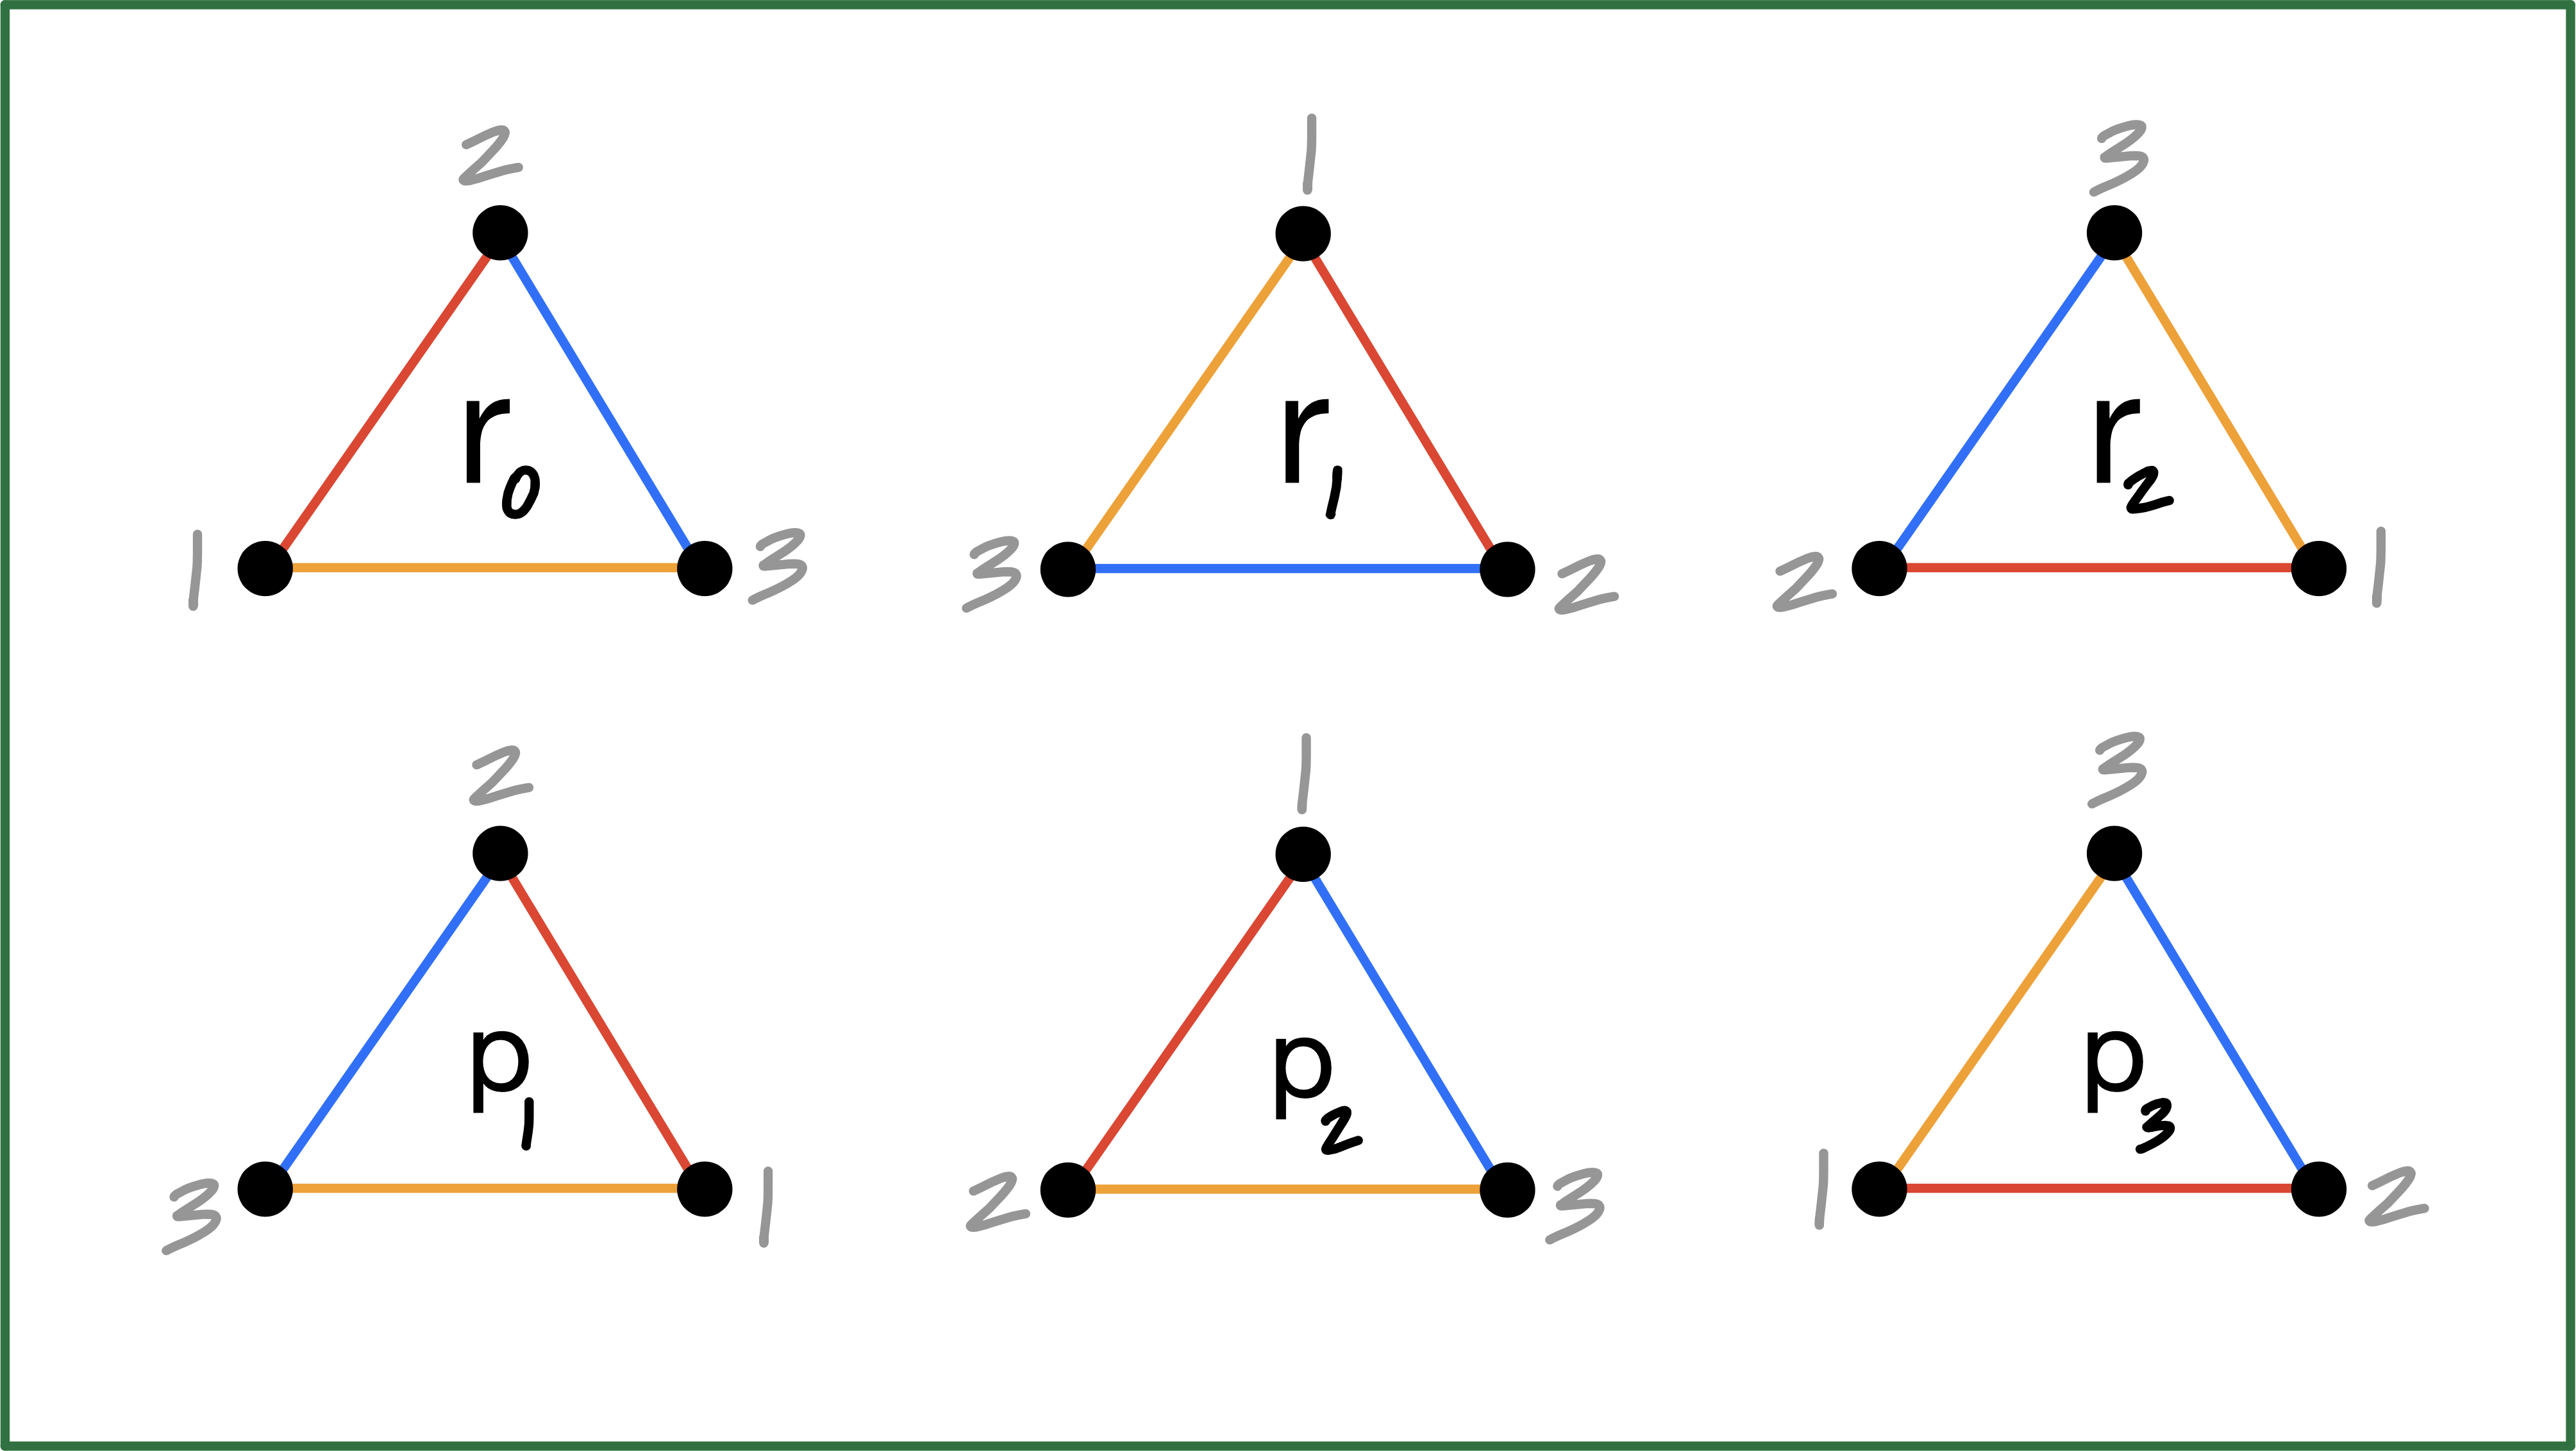
\includegraphics[width=0.5\linewidth]{permutationsoftriangle}
\end{center}

\p Think of the elements of $D_3$ as transformations of the \emph{default} or \emph{neutral} triangle $r_{0}$.  In particular,
\begin{align*}
r_0 &= \text{ clockwise rotation by }0^{\circ}\\
r_1 &= \text{ clockwise rotation by }120^{\circ}\\
r_2 &= \text{ clockwise rotation by }240^{\circ}\\
p_1 &= \text{ flip of the edge connecting vertices }1\text{ and }3\\
p_2 &= \text{ flip of the edge connecting vertices }1\text{ and }2\\
p_3 &= \text{ flip of the edge connecting vertices }2\text{ and }3
\end{align*}
\p Define the following product on $D_{3}$ as follows.  To multiply two elements $x,y\in D_3$, identify the flip or rotation that corresponds to $y$, and then perform it on $x$.  The result is assigned to the product $xy$.  For example,
\begin{center}
$r_{1}r_{1} = r_{2}$ and $r_{1}p_{2} = p_{3}$.
\end{center}
\p The complete multiplication table is given by
\bgroup
\begin{center}
\def\arraystretch{1.5}
\begin{tabular}{c|cccccc}
 & $r_{0}$ & $r_{1}$ & $r_{2}$ & $p_{1}$ & $p_{2}$ & $p_{3}$\\
\hline
$r_{0}$ & $r_{0}$ & $r_{1}$ & $r_{2}$ & $p_{1}$ & $p_{2}$ & $p_{3}$\\
$r_{1}$ & $r_{1}$ & $r_{2}$ & $r_{0}$ & $p_{3}$ & $p_{1}$ & $p_{2}$\\
$r_{2}$ & $r_{2}$ & $r_{0}$ & $r_{1}$ & $p_{2}$ & $p_{3}$ & $p_{1}$\\
$p_{1}$ & $p_{1}$ & $p_{3}$ & $p_{2}$ & $r_{0}$ & $r_{1}$ & $r_{2}$\\
$p_{2}$ & $p_{2}$ & $p_{1}$ & $p_{3}$ & $r_{2}$ & $r_{0}$ &$r_{1}$\\
$p_{3}$ & $p_{3}$ & $p_{2}$ & $p_{1}$ & $r_{1}$ & $r_{2}$ & $r_{0}$
\end{tabular}
\end{center}
\egroup
\p This product turns $D_{3}$ into a binary algebraic structure known as the \DEF{Dihedral Group on $3$ elements}, which may be generalized to $D_n$ for any $n\geq 3$.  You will study this more thoroughly in Math 3220.  
\end{enumerate}
\end{examples}
%
\begin{definition}
Let $(S,*)$ be a binary algebraic structure.  A subset $H\subset S$ is \DEF{closed under *} if $a*b\in H$ whenever $a,b\in H$.  In this case $\left(H,*\restrict{H\times H}\right)$ is also a binary algebraic structure, and is called a \DEF{sub-structure} of $(S,*)$.
\end{definition}
%
\terminology If the operation $*$ is clear from context, we may simply say that $H$ is a sub-structure of $S$, or that $H$ inherits an algebraic structure from $S$.
%
\begin{examples}~
\begin{enumerate}[(a)]
\item $R^{*} = \SET{x\in\REAL:x\neq 0}\subset \REAL$ is not closed under addition $+$, since $-1,1\in\REAL^{*}$ but $-1 + 1 = 0\notin \REAL^{*}$.  But $R^{*}$ is closed under multiplication, since if $x,y\in\REAL$ are both non-zero, then so is their product.  Hence $\REAL^{*}$ is a (multiplicative) sub-structure of $\REAL$.
\item The set $H = \SET{n^2:n\in\Z}\subset\Z$ is closed under multiplication.  Indeed if $x,y\in H$, then $x = m^2$ and $y=n^2$ for some $m,n\in\Z$.  So $xy = m^2n^2 = (mn)^2$, which is an element of $H$.  But $H$ is not closed under addition since, for example, $1 = 1^2\in H$ and $4 = 2^2\in H$, but $1 + 4 = 5\notin H$.
\end{enumerate}
\end{examples}
%
\begin{definition}
A binary operation $*$ on a set $S$ is
\begin{itemize}
\item \DEF{commutative} if $a*b = b*a$ for all $a,b\in S$, and
\item \DEF{associative} if $a*(b*c) = (a*b)*c$ for all $a,b,c\in S$.
\end{itemize}
\p In these cases, we may also say that $(S,*)$ is either commutative or associative, respectively.
\end{definition}
%
\begin{examples}~
\begin{enumerate}[(a)]
\item $(\Z,+)$ and $(\R,\cdot)$ are both commutative and associative.
\item $D_3$ is not commutative, since $r_1(p_1p_1) = r_1p_2 = p_3$ but $(r_1p_1)p_1 = p_3p_1 = r_1$.
\item The binary operation $*$ on $S = \SET{0,1}$ defined by 
\begin{center}
\def\arraystretch{1.5}
\begin{tabular}{c|cc}
$*$ & $0$ & $1$\\
\hline
$0$ & $1$ & $0$\\
$1$ & $1$ & $0$
\end{tabular}
\end{center}
\p is neither commutative nor associative, since $0*(0*1) = 0*0=1$ but $(0*0)*1 = 1*1=0$.
\end{enumerate}
\end{examples}
%
\subsection{Isomorphic Binary Structures}

\recall If $X$ and $Y$ are any sets, a map $f:X\to Y$ is said to be
\begin{itemize}
\item \DEF{injective} or \DEF{one-to-one} if whenever $f(x_{1}) = f(x_{2})$, we have $x_{1} = x_{2}$.
\item \DEF{surjective} or \DEF{onto} if for all $y\in Y$, there exists $x\in X$ such that $f(x) = y$.
\end{itemize}
%
\begin{definition}
Let $(S,*)$ and $(S',*')$ be binary algebraic structures.  A bijection $\varphi:S\to S'$ is an \DEF{isomorphism} if $\varphi(a*b) = \varphi(a)*'\varphi(b)$ for all $a,b\in S$.  In this case we say that $(S,*)$ and $(S',*')$ are \DEF{isomorphic}.
\end{definition}
\vsp

\notation If $(S,*)$ and $(S',*')$ are isomorphic, we write $(S,*)\cong(S',*')$.
\vsp

%
\begin{example}\label{firstisomorphismexample}
Let $S = \SET{a,b,c}$ and $S' = \SET{1,2,3}$ be binary algebraic structures under the operations $*$ and $*'$ respectively defined by the following tables:
\begin{center}
\bgroup
\begin{center}
\def\arraystretch{1.5}
\begin{tabular}{c|ccc}
$*$ & $a$ & $b$ & $c$\\
\hline
$a$ & $b$ & $a$ & $c$\\
$b$ & $a$ & $c$ & $b$\\
$c$ & $c$ & $b$ & $a$\\
\end{tabular}
\hspace{3cm}
\begin{tabular}{c|ccc}
$*'$ & $1$ & $2$ & $3$\\
\hline
$1$ & $2$ & $1$ & $3$\\
$2$ & $1$ & $3$ & $2$\\
$3$ & $3$ & $2$ & $1$\\
\end{tabular}
\end{center}
\egroup
\end{center}
\p A close examination of these tables results in the conclusion that the only difference between the binary structures $(S,*)$ and $(S', *')$ is the way the elements are labelled.  If we define $\varphi:S\to S'$ by
\begin{center}
$\varphi(a) = 1, \varphi(b) = 2$, and $\varphi(c) = 3$
\end{center}
it may be checked that $\varphi$ is an isomorphism.  For example
\begin{center}
$\varphi(a*b) = \varphi(a) = 1 = 1*' 2 = \varphi(a)*'\varphi(b)$.
\end{center}
\p But it must also be verified that $\varphi(a*c) = \varphi(a)*'\varphi(c)$ and $\varphi(b*c) = \varphi(b)*'\varphi(c)$.  But even still there are other products to consider!  Only after checking that $\varphi(a*a) = \varphi(a)*'\varphi(a), \ \ \varphi(b*b) = \varphi(b)*'\varphi(b)$, and $\varphi(c*c) = \varphi(c)*'\varphi(c)$, may we finally conclude that $\varphi$ is an isomorphism and that $S\cong S'$.  These checks are left to you as an exercise.
\end{example}
%
\begin{exercise}
The set $2\Z := \SET{2n:n\in\Z} = \SET{0, \pm 2, \pm 4,\ldots}$ of even integers is a binary algebraic structure under addition.  Prove that $(\Z,+)\cong (2\Z,+)$.
\end{exercise}
%
\notation For $a,n\in\Z$ with $n\neq 0$, let $a\text{ mod }n$ denote the remainder when $a$ is divided by $n$.  For example, $15\text{ mod }4 = 3$ and $8\text{ mod }2 = 0$.
%
\begin{examples}~
\begin{enumerate}[(a)]
\item Let $n>0$ be an integer, and recall that in Definition \ref{congruenceoperations}, the set $\ZN = \SET{[a]:a\in\INTEGER}$ of congruence classes modulo $n$ was introduced and equipped with addition and multiplication operations defined by
\begin{center}
$[a]\oplus [b] = [a + b]$ and $[a]\odot [b] = [ab]$, for all $[a],[b]\in\ZN$.
\end{center}
\p Note that $(\ZN,\oplus)$ and $(\ZN,\odot)$ are both binary algebraic structures.
\vsp

\p Consider now the set $\overline{\Z}_{n} = \SET{0,1,2,\ldots, n-1}$, which is also a binary algebraic structure under either of the addition $+_{n}$ and multiplication $\cdot_{n}$ operations defined by
\begin{center}
$a+_{n}b = (a + b)\text{ mod }n$,
\end{center}
and
\begin{center}
$a\cdot_{n}b = (ab)\text{ mod }n$, for all $a,b\in\overline{\Z}_{n}$.
\end{center}

\p The differences between $\overline{\Z}_{n}$ and the $\ZN$ are merely cosmetic!  Indeed define $\varphi:\overline{\Z}_{n}\to \Z_{n}$ by $\varphi(a) = [a]$ for all $a \in \overline{\Z}_{n}$.  By Corollary \ref{elementsofZn}, $\varphi$ is a bijection.  Moreover, for any $a,b\in\overline{\Z}_{n}$, we have 
\begin{center}
$\varphi(a+_nb) = \varphi\big((a+b)\text{ mod }n\big) = [(a+b)\text{ mod }n] = [a+b] = [a]\oplus [b] = \varphi(a)\oplus\varphi(b)$,
\end{center}
and
\begin{center}
$\varphi(a\cdot_nb) = \varphi\big((ab)\text{ mod }n\big) = [(ab)\text{ mod }n] = [ab] = [a]\odot [b] = \varphi(a)\odot\varphi(b)$.
\end{center}
%
\p Hence $(\ZN,\oplus)$ is isomorphic to $(\overline{\Z}_n,+_n)$ and $(\ZN,\odot)$ is isomorphic to $(\overline{\Z}_n,\cdot_n)$.  From now on, we will ignore the distinction between the sets $\overline{\Z}_n$ and $\ZN$ and simply write $\ZN$ to refer to whichever one is more convenient to work with in the moment.  We will also use the more traditional $+$ and $\cdot$ to represent addition and multiplication in $\ZN$, respectively.
%
\item The set $\REAL^{+} = \SET{x\in\REAL:x>0}$ is a binary algebraic structure under multiplication.  It may be seen that $(\REAL^{+},\cdot)$ is isomorphic to $(\REAL, +)$ since the map $\varphi:\REAL\to\REAL^{+}$ defined by $\varphi(x) = e^{x}$ is a bijection, and $\varphi(x+y) = e^{x + y} = e^xe^{y} = \varphi(x)\varphi(y)$, for any $x,y\in\REAL$.
%
\item For any integer $n>0$, the set $U_{n} = \SET{z\in\COMPLEX:z^n = 1}$ of $n$th roots of unity is a binary algebraic structure under multiplication, since if $z_{1},z_{2}\in U_{n}$, we must have $z_{1}^n = 1$ and $z_{2}^n = 1$.  Hence $z_{1}z_{2}\in U_n$ since $(z_{1}z_{2})^n = z_{1}^nz_{2}^n = 1\cdot 1 = 1$.  It turns out that $(U_{n},\cdot)$ is isomorphic to $(\ZN,+)$!
\vsp

\p To see why this is the case, recall Theorem \ref{rootsofunityclassification} which says that
\begin{center}
$U_{n} = \SET{\xi^{k}:k=0,1,2\ldots, n-1}$,
\end{center}
where $\xi = e^{i(2\pi/n)} = \cos(2\pi/n) + i\sin(2\pi/n)$.  Define $\varphi:U_{n}\to\ZN$ by $\varphi(\xi^k) = k$.  It is immediate that $\varphi$ is a bijection, and for any $\xi^{k_1},\omega^{k_2}\in U_n$ we have
\begin{center}
$\varphi(\omega^{k_1}\omega^{k_2}) = \varphi(\xi^{k_1+k_2}) = k_1+k_2 = \varphi(\xi^{k_1}) + \varphi(\xi^{k_1})$.
\end{center}
\end{enumerate}
\end{examples}
%
\begin{lemma}\label{selfsquarelemma}
Suppose $(S,*)$ and $(S',*')$ are isomorphic binary algebraic structures, and that there exists a unique $x\in S$ such that $x*x = x$.  Prove that there exists a unique $y'\in S'$ such that $y'*'y' = y'$.
\end{lemma}
%
\begin{proof}\phantom{-}

\p (Existence) By assumption, there exists an isomorphism $\varphi:S\to S'$.  Take $y' = \varphi(x)$ and check that $y'*y' = \varphi(x)*'\varphi(x) = \varphi(x*x) = \varphi(x) = y'$.
\vsp

\p (Uniqueness) Suppose for a contradiction that there exists $y_{1}',y_{2}'\in S'$ with $y_{1}'\neq y_{2}'$ such that $y_{1}'*'y_{1}' = y_{1}'$ and $y_{2}'*'y_{2}' = y_{2}'$.  Then set $x_{1} = \varphi^{-1}(y_{1}')$ and $x_{2} = \varphi^{-1}(y_{2}')$ and note that
\begin{center}
$x_{1}*x_{1} = \varphi^{-1}\big(\varphi(x_1*x_1\big) = \varphi^{-1}\big(\varphi(x_1)*'\varphi(x_1)\big) = \varphi^{-1}\big(y_{1}'*'y_{1}'\big) = \varphi^{-1}(y_{1}') = x_{1}$
\end{center}
and similarly
\begin{center}
$x_{2}*x_{2} = \varphi^{-1}\big(\varphi(x_2*x_2\big) = \varphi^{-1}\big(\varphi(x_2)*'\varphi(x_2)\big) = \varphi^{-1}\big(y_{2}'*'y_{2}'\big) = \varphi^{-1}(y_{2}') = x_{2}$.
\end{center}
Since $\varphi$ is a bijection and $y_{1}'\neq y_{2}'$, we must have $x_{1}\neq x_{2}$, this is a contradiction.
\end{proof}
%
\begin{theorem}
$(\Z,+)$ and $(\Z,\cdot)$ are not isomorphic.
\end{theorem}
%
\begin{proof}
The equation $x + x = x$, has only one integer solution, namely $x = 0$.  But both $0$ and $1$ are integer solutions to the equation $x\cdot x = x$.  Therefore the result follows by Lemma \ref{selfsquarelemma}.
\end{proof}
%
\begin{definition}
Let $(S,*)$ be a binary algebraic structure.  $e\in S$ is an \DEF{identity element} for $*$ if $e*x = x$ and $x*e = x$ for all $x\in S$.
\end{definition}
%
\begin{examples}~
\begin{enumerate}[(a)]
\item In $(\Z,+)$, $0$ is the identity element.
\item In $(\REAL,\cdot)$, $1$ is the identity element.
\item In $D_3$, $r_{0}$ is the identity element (see Example \ref{basexamples} \ref{dihedralgroup}).
\item In $M_{2}(\REAL)$, $\MATRIX{rr}{1 & 0\\0 & 1}$ is the identity element.
\item The binary algebraic structure $(S,*)$ from Example \ref{firstisomorphismexample} has no identity element.
\end{enumerate}
\end{examples}
%
\begin{remark}\label{uniqueidentities}
A binary algebraic structure $(S,*)$ can have at most one identity element $e$, for if $e'\in S$ is also an identity element, then $e = e*e' = e'$.
\end{remark}
%
\begin{exercise}
Suppose $(S,*)$ and $(S',*')$ are two isomorphic binary algebraic structures.  Prove that if $S$ has an identity element for $*$, that $S'$ has an identity element for $*'$.
\end{exercise}

\subsection{Definition and Examples of Rings}

\begin{definition}\label{ringdefinition}
A \DEF{ring} is a set $R$ with two binary operations $+$ and $\cdot$ satisfying the following properties.
\begin{enumerate}[(1)]
\item $a + b = b + a$, for all $a,b\in R$.\label{commutativityofaddition}
\item $a + (b + c) = (a + b) + c$, for all $a,b,c\in R$.\label{associativityofaddition}
\item There exists $0_{R}\in R$ such that $a + 0_{R} = a$ for all $a\in R$.\label{additiveidentity}
\item For every $a\in R$, there exists $b\in R$ such that $a + b = 0_{R}$.\label{additiveinverse}
\item $a\cdot(b\cdot c) = (a\cdot b)\cdot c$, for all $a,b,c\in R$.\label{associativityofmultiplication}
\item $a\cdot(b + c) = a\cdot b + a\cdot c$, for all $a,b,c\in R$.\label{leftdistributivity}
\item $(a + b)\cdot c = a\cdot c + b\cdot c$, for all $a,b,c\in R$.\label{rightdistributivity}
\end{enumerate}
\end{definition}
%
\begin{remarks}~
\begin{enumerate}[(1)]
\item The element $0_{R}$ whose existence was postulated in property \ref{additiveidentity} is referred to as the \DEF{additive identity} or \DEF{zero element} of $R$.  This element is unique.  Indeed, similar to the comments made in in Remark \ref{uniqueidentities}, if $0_{R}'\in R$ is another additive identity, then $0_{R} = 0_{R} + 0_{R}' = 0_{R}'$.  When there is no risk of confusion, we drop the subscript and simply denote it by $0$.

\item The element $b$ mentioned in property \ref{additiveinverse} is called the \DEF{additive inverse} of $a$, and is typically denoted by $-a$.  It is also unique, since if $b$ and $b'$ satisfy $a + b = 0$ and $a + b' = 0$, then
\begin{center}
$b = b + 0 = b + (a + b') = (b + a) + b' = (a + b) + b' = 0 + b' = b'$.
\end{center}
\item While subtraction was not explicitly mentioned in Definition \ref{ringdefinition}, we may define it over a ring $R$ by
\begin{center}
$a - b = a + (-b)$, for all $a,b\in R$.
\end{center}
\item As usual, the concatenation $ab$ is often used to represent the product $a\cdot b$ of $a,b\in R$.
\item It follows from the properties listed in Definition \ref{ringdefinition} that $0a = 0$ for any $a\in R$.  Indeed by \ref{rightdistributivity}, we have
\begin{center}
$0a = (0 + 0)a = 0a + 0a$.
\end{center}
It follows that $0a = 0a + 0 = 0a + (0a - 0a) = (0a + 0a) - 0a = 0a - 0a = 0$.
\item Formally speaking, a ring is defined to be a triple $(R,+,\cdot)$, where $(R,+)$ and $(R,\cdot)$ are both binary algebraic structures satisfying the properties listed in Definition \ref{ringdefinition}.  But usually we will casually refer to the set $R$ itself as a ring, with the understanding that it must come equipped with the operations $+$ and $\cdot$.
\end{enumerate}
\end{remarks}
%
\begin{exercises}\label{ringpropertyexercises} Prove the following statements about a ring $R$.
\begin{enumerate}[(a)]
\item $a(b-c) = ab - ac$ and $(a-b)c = ac - bc$ for all $a,b,c\in R$.
\item $-(-a) = a$ for all $a\in R$.
\item $a(-b) = -(ab) = (-a)b$ for all $a,b\in R$.\label{negativeproduct}
\item $-(a+b) = -a - b$ for all $a,b\in R$.
\item $-(a-b) = b-a$ for all $a,b\in R$.
\item $(-a)(-b) = ab$ for all $a,b\in R$.
\end{enumerate}
\end{exercises}
%
\p In particular, a consequence of Exercise \ref{ringpropertyexercises} \ref{negativeproduct} that $-a = (-1)a$ for any $a\in R$.
\vsp

\terminology
\begin{itemize}
\item If $a\cdot b = b\cdot a$ for all $a,b\in R$, then $R$ is said to be \DEF{commutative}.
\item A ring $R$ is said to be \DEF{unital} or a \DEF{ring with identity} if there exists $1_{R}\in R$ such that $1_{R}\cdot a = a$ and $a\cdot 1_{R} = a$ for all $a\in R$.  This element $1_{R}$ is called the \DEF{multiplicative identity} or \DEF{unity} of $R$, and may be denoted as $1$, whenever there is no risk of confusion.
\end{itemize}
%
\begin{examples}\label{ringexamples}~
\begin{enumerate}[(a)]
\item $\Z, \RATIONAL, \REAL$ and $\COMPLEX$, equipped with the standard addition and multiplication operations are all commutative unital rings.
\item Whenever $n\in\Z$ with $n > 0$, $\ZN$ is a commutative unital ring by Theorem \ref{propertiesofZn}.
\item\label{Rsquared} $\REAL^{2} = \SET{(a,b):a,b\in\REAL}$ is a commutative ring with addition $+$ and multiplication $\cdot$ defined by
\begin{center}
$(a_1,b_1) + (a_2,b_2) = (a_1 + a_2,b_1 + b_2)$ and $(a_1,b_1) \cdot (a_2,b_2) = (a_1a_2,b_1b_2)$
\end{center}
for all $(a_1,b_1), (a_2,b_2)\in\REAL^{2}$.  Moreover, $\REAL^{2}$ is unital with identity $1_{\REAL^{2}} = (1,1)$.
\item The set $M_{2}(\REAL) = \SET{\MATRIX{rr}{a & b\\c&d}:a,b,c,d\in\REAL}$ of all $2\BY 2$ matrices with real entries is a ring.

\p Addition and multiplication are defined using the rules
\begin{center}
$\MATRIX{rr}{a_1 & b_1\\c_1 & d_1} + \MATRIX{rr}{a_2 & b_2\\c_2 & d_2} = \MATRIX{cc}{a_1 + a_2 & b_1 + b_2\\c_1 + c_2& d_1 + d_2}$
\end{center}
and
\begin{center}
$\MATRIX{rr}{a_1 & b_1\\c_1 & d_1}\MATRIX{rr}{a_2 & b_2\\c_2 & d_2} = \MATRIX{cc}{a_1a_2 + b_1b_2 & a_1c_2 + b_1d_2\\c_1a_2 + d_1b_2 & c_1b_2 + d_1d_2}$,
\end{center}
\p $M_{2}(\REAL)$ is not commutative, since
\begin{center}
$\MATRIX{rr}{1 & 1\\-1 & 1}\MATRIX{rr}{1 & 1\\2 & 1} = \MATRIX{rr}{3 & 2\\1 & 0}$
\end{center}
but
\begin{center}
$\MATRIX{rr}{1 & 1\\2 & 1}\MATRIX{rr}{1 & 1\\-1 & 1} = \MATRIX{rr}{0 & 2\\ 1 & 3}$,
\end{center}
\p but it is unital with multiplicative identity given by $1_{M_{2}(\REAL)} = \MATRIX{rr}{1 & 0\\0 & 1}$.
\item The set $F(\REAL)$ of all functions $f:\REAL\to\REAL$ is a commutative ring, when equipped with point-wise addition and multiplication:
\begin{center}
$(f+g)(x) = f(x) + g(x)$
\end{center}
and
\begin{center}
$(fg)(x) = f(x)g(x)$,
\end{center}
for all $f,g\in F(\REAL)$.  $F(\REAL)$ is also unital with $1_{F(\REAL)}$ equal to the constant function which is identically $1$ on $\REAL$.
\item The singleton $R = \SET{0}$ is a ring, with addition and multiplication operations defined by $0 + 0 = 0$ and $0\cdot 0 = 0$.  And it may be odd to say so, but $R$ is in fact unital, since $0$ satisfies the definition of both the additive and multiplicative identity!  In this case $R$ is called the \DEF{zero ring}, or \DEF{null ring} and is sometimes written as $R = 0$.  Any other ring is said to be \DEF{non-zero}.
\end{enumerate}
\end{examples}
%
\begin{exercise}
Show that $(F(\REAL), +, \circ)$ fails to be a ring when $\oplus$ represents point-wise addition and $\circ$ corresponds to function composition.
\end{exercise}
%
\begin{definition}
Let $R$ be a ring.  A subset $S\subset R$ is a \DEF{subring} of $R$ if it is a ring when equipped with the operations inherited from $R$.
\end{definition}
%
\begin{example}
$\Z$ is a subring of $\RATIONAL$, $\RATIONAL$ is a subring of $\REAL$, and $\REAL$ is a subring of $\COMPLEX$.
\end{example}
%
\begin{remarks}~
\begin{enumerate}[(a)]
\item Note that if $R$ is any ring, then both $R$ and the zero ring are automatically subrings of $R$.  Any other subring of $R$ is said to be \DEF{proper}.
\item A subring $S$ of a commutative ring $R$ is commutative.  Since if
\begin{center}
$ab = ba$ for all $a,b\in R$,
\end{center}
then the weaker statement
\begin{center}
$ab = ba$ for all $a,b\in S$
\end{center}
must be true as well, as the elements of $S$ are among those in $R$.
\end{enumerate}
\end{remarks}
%
\begin{theorem}[Subring Criterion]\label{subringcriterion}
If $R$ is a ring, then any subset $S\subset R$ is a subring of $R$ if:
\begin{enumerate}[(1)]
\item $a+b\in S$ and $ab\in S$ whenever $a,b\in S$
\item $0_{R}\in S$
\item $-a\in S$ whenever $a\in S$.
\end{enumerate}
\end{theorem}
%
\begin{proof}
We directly verify that any subset $S\subset R$ satsifying $(1)-(3)$ above, automatically satisfies all of the properties listed in Definition \ref{ringdefinition}.
\begin{enumerate}[(1)]
\item Since $a + b = b + a$ for every $a,b\in R$, this equation certainly holds for all $a,b\in S$.
\item Similarly, $a + (b +c)  = (a + b) + c$ holds for every $a,b,c\in R$, so it must hold for every $a,b,c\in S$.
\item The existence of $0_{S}\in S$ such that $0_{S} + a = a$ for all $a\in S$ is guaranteed by assumption (2) which says that $0_R\in S$.  Simply take $0_S = 0_R$.
\item For each $a\in S$, assumption (3) guarantees that $-a\in S$.  Hence the requirement for additive inverses is immediately satisfied.
\item Since $a\cdot(b\cdot c) = (a\cdot b)\cdot c$ for every $a,b,c\in R$, it must also hold for every $a,b,c\in S$.
\item $a\cdot (b + c) = a\cdot b + a\cdot c$ for every $a,b,c\in S$, because the same equation holds for all $a,b,c\in R$.
\item Similarly, $(a + b)\cdot c = a\cdot c + b\cdot c$ for every $a,b,c\in R$ so it must hold for every $a,b,c\in S$.\qedhere
\end{enumerate}
\end{proof}
\smsp

%
\begin{example}\label{abnegativebasubring}
The set
\begin{center}
$S = \SET{\MATRIX{rr}{a & b\\-b & a}:a,b,\in\REAL}$
\end{center}
is a subring of $M_{2}(\REAL)$, which may be proved using the Subring Criterion.  First, suppose $A,B\in S$ and choose $a_{1},b_{1},a_{2},b_{2}\in\REAL$ such that
\begin{center}
$A = \MATRIX{rr}{a_{1} & b_{1}\\-b_{1} & a_{1}}$ and $B = \MATRIX{rr}{a_{2} & b_{2}\\-b_{2} & a_{2}}$.
\end{center}
It follows that
\begin{center}
$A + B = \MATRIX{rr}{a_{1} & b_{1}\\-b_{1} & a_{1}} + \MATRIX{rr}{a_{2} & b_{2}\\-b_{2} & a_{2}} =  \MATRIX{rr}{\phantom{-(}a_{1} + a_{2}\phantom{)}& b_{1} + b_{2}\\-(b_{1} + b_{2}) & a_{1} + a_{2}}\in S$
\end{center}
and
\vsp

\begin{adjustwidth}{-100pt}{-100pt}
\begin{center}
$AB = \MATRIX{rr}{a_{1} & b_{1}\\-b_{1} & a_{1}}\MATRIX{rr}{a_{2} & b_{2}\\-b_{2} & a_{2}} = \MATRIX{cc}{\phantom{-}a_1a_2 - b_1b_2 & \phantom{-}a_1b_2 + b_1a_2\\-b_1a_2-a_1b_2 & -b_1b_2 + a_1a_2} = \MATRIX{cc}{\phantom{-(}a_1a_2 - b_1b_2\phantom{)} & a_1b_2 + b_1a_2\\-(a_1b_2 + b_1a_2) & a_1a_2 - b_1b_2}\in S$.
\end{center}
\end{adjustwidth}
\vsp

\p To see that (2) holds, note that the additive identity in $M_2(\REAL)$ is (the \DEF{zero matrix}) given by
\begin{center}
$O = \MATRIX{rr}{0 & 0\\0 & 0}$,
\end{center}
which is also in $S$ since
\begin{center}
$O = \MATRIX{rr}{0 & 0\\0 & 0} = \MATRIX{rr}{a & b\\-b & a}$, where $a = 0$ and $b = 0$.
\end{center}
\p Finally, if $A = \MATRIX{rr}{a & b\\-b & a}\in S$, then $-A = \MATRIX{rr}{-a & -b\\b & -a} = \MATRIX{cc}{-a & -b\\-(-b) & -a}\in S$, which verifies $(3)$.
\end{example}

\begin{exercise}\label{zadjoinroottwosubringofreal}
Show that $\Z[\sqrt{2}] = \SET{a + b\sqrt{2}:a,b\in\Z}$ is a subring of $\REAL$.
\end{exercise}
%
\begin{definition}
Let $R$ and $S$ be rings.  The \DEF{Cartesian product} of $R$ and $S$ is defined as
\begin{center}
$R\times S = \SET{(r,s):r\in R,s\in S}$,
\end{center}
equipped with addition and multiplication defined by
\begin{center}
$(r_1,s_1) + (r_2,s_2) = (r_1 + r_2,s_1 + s_2)$ and $(r_1,s_1)\cdot(r_2,s_2) = (r_1r_2,s_1s_2)$
\end{center}
for all $(r_1,s_1),(r_2,s_2)\in R\times S$.
\end{definition}
%
\begin{remarks}~
\begin{enumerate}[(1)]
\item The additive identity for $R\times S$ is given by $0_{R\times S} = (0_{R},0_{S})$.
\item The additive inverse of any $(r,s)\in R\times S$ is given by $-(r,s) = (-r,-s)$.
\item If $R$ and $S$ are unital, then so is $R\times S$, with $1_{R\times S} = (1_{R},1_{S})$.
\end{enumerate}
\end{remarks}
%
\begin{example}~
%\item In Examples \ref{ringexamples} \ref{Rsquared} we defined the ring $\REAL^{2}$, which is no different than the Cartesian product $\REAL\times\REAL$.
Consider the the Cartesian product
\begin{center}
$\Z_{5}\times M_{2}(\REAL) =\SET{(n,A):n\in\Z_5, A\in M_{2}(\REAL)}$,
\end{center}
and choose two elements in particular, say
\begin{center}
$\left(4, \MATRIX{rr}{1 & 1\\3 & 5}\right)$ and $\left(2, \MATRIX{rr}{-1  & 1\\0 & 1}\right)$.
\end{center}
We may add them by computing
\begin{center}
$\left(4, \MATRIX{rr}{1 & 1\\3 & 5}\right) + \left(2, \MATRIX{rr}{-1  & 1\\0 & 1}\right) = \left(4 + 2, \MATRIX{rr}{1 & 1\\3 & 5} + \MATRIX{rr}{-1  & 1\\0 & 1}\right) = \left(1, \MATRIX{rr}{0 & 2\\3 & 6}\right)$
\end{center}
or multiply them as
\begin{center}
$\left(4, \MATRIX{rr}{1 & 1\\3 & 5}\right)\cdot \left(2, \MATRIX{rr}{-1  & 1\\0 & 1}\right) = \left(4\cdot 2, \MATRIX{rr}{1 & 1\\3 & 5}\MATRIX{rr}{-1  & 1\\0 & 1}\right) = \left(3, \MATRIX{rr}{-1 & 2\\-3 & 8}\right)$.
\end{center}
\p Since $\Z_{5}$ and $M_{2}(\REAL)$ are both unital, so is $\Z_{5}\times M_{2\BY 2}(\REAL)$ with identity $\left(1,\MATRIX{rr}{1 & 0\\0 & 1}\right)$.
\end{example}
%
\subsection{Integral Domains and Fields}
%
\begin{definition}
Let $R$ be a ring.  An element $a\in R$ is a \DEF{zero divisor} if there exists a non-zero $b\in R$ such that $ab = 0$.  In this case $b$ is also a \DEF{zero divisor}.
\end{definition}
%
\begin{definition}
A non-zero commutative unital ring is an \DEF{integral domain} if it has no zero divisors.
\end{definition}
%
\begin{examples}~
\begin{enumerate}[(a)]
\item $\Z, \RATIONAL, \REAL$, and $\COMPLEX$ are all integral domains.
\item By Theorem \ref{primepnozerodivisors}, if $p$ is prime, $\Z_p$ is an integral domain.
\item $\Z_{30}$ is not an integral domain.  Indeed $2$ and $15$ are zero divisors since $2\cdot 15 = 30 = 0$ in $\Z_{30}$.
\vsmsp

\p More generally, any composite integer $n>1$ can be factored as $n = mk$ for some integers $m$ and $k$ with $1 < m\leq k < n$.  It follows that $m$ and $k$ are zero divisors since $mk = n = 0$ in $\ZN$, so $\ZN$ contains zero divisors and is hence not an integral domain.
\item $M_{2}(\REAL)$ is not an integral domain, since $\MATRIX{rr}{1 & 0\\0 & 0}\MATRIX{rr}{0 & 0\\0 & 1} = \MATRIX{rr}{0 & 0\\0 & 0}$.
\end{enumerate}
\end{examples}
%
\begin{exercise}
Let $R$ and $S$ be rings.  Prove that the Cartesian product $R\times S$ is an integral domain if and only if both $R$ and $S$ are integral domains.
\end{exercise}
%
\begin{definition}
Let $R$ be a unital ring (not necessarily commutative).  An element $a\in R$ is a \DEF{unit} if there exists $b\in R$ such that $ab = 1$ and $ba = 1$.  In this case, we call $b$ the \DEF{multiplicative inverse} of $a$.
\end{definition}
%
\begin{remark}
Multiplicative inverses are unique!  Indeed if $b_{1},b_{2}\in R$ both satisfy $ab_{1} = ab_{2} = 1$ and $b_{1}a = b_{2}a = 1$, then we must have
\begin{center}
$b_1 = 1\cdot b_1 = (b_2a)b_1 = b_2(ab_1) = b_2\cdot 1 = b_2$.
\end{center}
\end{remark}
%
\begin{examples}~
\begin{enumerate}[(a)]
\item In $\Z$, the only units are $1$ and $-1$.
\item By Lemma \ref{gcdunitlemma}, $a\in \ZN$ is a unit if and only if $\GCD{a,n} = 1$.
\item In $\RATIONAL$ and $\REAL$, every non-zero element is a unit.
\item By Theorem \ref{Znallunits}, every non-zero element of $\Z_p$ is a unit whenever $p$ is prime.
\item In $M_{2}(\REAL)$, the units are the matrices with non-zero determinants.  That is, the matrices of the form
\begin{center}
$\MATRIX{rr}{a & b\\c & d}$
\end{center}
satisfying $ad - bc \neq 0$.
\end{enumerate}
\end{examples}
%
\begin{exercise}
Let $R$ be a ring.  Is the set $U=\SET{a\in R:a\text{ is a unit}}$ a subring of $R$?
\end{exercise}
%
\begin{lemma}\label{unitscantbezerodivisors}
If $R$ is a unital ring, and then no unit can be be a zero divisor.
\end{lemma}
%
\begin{proof}
If $a\in R$ is a unit and a zero divisor, we could choose non-zero $b\in R$ such that $ab = 0$.  But then
\begin{center}
$b = (a^{-1}a)b = a^{-1}(ab) = a^{-1}\cdot 0 = 0$,
\end{center}
which is a contradiction.
\end{proof}
%
\begin{definition}
A \DEF{field} $F$ is a non-zero commutative unital ring with the property that every non-zero element $a\in F$ is a unit.
\end{definition}
%
\begin{examples}~
\begin{enumerate}[(a)]
\item $\RATIONAL, \REAL$, and $\COMPLEX$ are all fields.
\item $\Z$ is not a field, since $2$ has no inverse.
\item In a manner similar to Exercise \ref{zadjoinroottwosubringofreal}, it may be checked that $\RATIONAL[\sqrt{2}] = \SET{a + b\sqrt{2}:a,b\in\RATIONAL}$ is a subring of $\REAL$, and in fact it is a field!  Certainly $\RATIONAL[\sqrt{2}]$ is commutative as it is a subring of $\REAL$, and it is unital, since $1 = 1 + 0\sqrt{2}\in\RATIONAL[\sqrt{2}]$.  Finally, we verify that any non-zero $a+b\sqrt{2}\in \RATIONAL[\sqrt{2}]$ is a unit.  Of course in $\REAL$ we may compute
\begin{center}
$(\ds{a + b\sqrt{2})\left(\frac{1}{a + b\sqrt{2}}\right) = 1}$.
\end{center}
So all that need be checked is that $\dfrac{1}{a + b\sqrt{2}}\in \RATIONAL[\sqrt{2}]$, and indeed
\begin{center}
$\ds{\frac{1}{a + b\sqrt{2}} = \frac{1}{a + b\sqrt{2}}\cdot\frac{a - b\sqrt{2}}{a - b\sqrt{2}} = \frac{a - b\sqrt{2}}{a^2 + 2b^2} = \underbrace{\frac{a}{a^2 + 2b^2}}_{\in\RATIONAL} + \underbrace{\frac{-b}{a^2 + 2b^2}}_{\in\RATIONAL}\sqrt{2}\in\RATIONAL[\sqrt{2}]}$.
\end{center}
\end{enumerate}
\end{examples}
%
\begin{theorem}\label{fieldisdomain}
Every field is an integral domain.
\end{theorem}
%
\begin{proof}
If $F$ is a field, then it is already a non-zero commutative unital ring.  So all that is left to show is that $F$ has no zero divisors.  But every non-zero $a\in F$ is a unit.  So by Lemma \ref{unitscantbezerodivisors}, $F$ cannot be a zero divisor.
\end{proof}
%
\begin{remark}
Note that the converse of Theorem \ref{fieldisdomain} is false, with $\Z$ serving as a counter-example.
\end{remark}
%
\begin{theorem}
A finite integral domain $D$ is a field.
\end{theorem}
%
\begin{proof}
Let $D^{*} = \SET{a\in D:a\neq 0}$ and define for each $a\in D^*$ the map $\lambda_{a}:D^{*}\to D^{*}$ by $\lambda_{a}(x) = ax$.  Note that $\lambda_{a}$ is a bijection.  To see injectivity, suppose $\lambda_{a}(x_{1}) = \lambda_{a}(x_{2})$.  It follows that
\begin{center}
$a(x_{1} - x_{2}) = ax_1 - a_x2 =  \lambda_{a}(x_{1}) - \lambda_{a}(x_{2}) = 0$.
\end{center}
Since $a\neq 0$, it cannot be a zero divisor and hence $x_{1} - x_{2} = 0$, or equivalently, $x_{1} = x_{2}$.  To see surjectivity, suppose for a contradiction that $y\in D^{*}$ such that $\lambda_{a}(x)\neq y$ for all $x\in D^{*}$.  Since $\lambda_{a}$ is injective, the set
\begin{center}
$\lambda_{a}(D^{*}) = \SET{\lambda_{a}(x):x\in D^{*}}$
\end{center}
has the same number of elements as $D^{*}$.  But by assumption $y\notin \lambda_{a}(D^{*})$, so
\begin{center}
$\lambda_{a}(D^{*})\cup \SET{y}$
\end{center}
is a subset of $D^{*}$ with more elements than $D^{*}$.  This is a contradiction.
\vsp

\p Returning to the main claim, since $\lambda_{a}$ is a bijection, $\lambda_{a}(D^{*}) = D^{*}$, which contains $1$.  Hence there exists $x\in D^{*}$ such that $ax = \lambda_{a}(x) = 1$.  It follows that $a$ is a unit, and since $a$ was chosen to be an arbitrary non-zero element of $D$, $D$ must be a field.  
\end{proof}
\vsp

\subsection{Cancellation Properties}

\p When faced with an integer equation such as $x + 3 = y + 3$, we often cancel the $3$'s without hesitation and conclude that $x = y$.  This is usually justified by saying that we are \emph{subtracting $3$} from both sides of the equation, a possibility which generalizes to any ring.

\begin{theorem}[Additive Cancellation]\label{additivecancellation}
If $R$ is a ring, and $a,b,c\in R$ such that
\begin{center}
$a + c = b + c$,
\end{center}
then $a = b$.
\end{theorem}
%
\begin{proof}
If $a + c = b + c$, then $a = a + 0 = a + (c - c) = (a + c) - c = (b + c) - c = b + (c - c) = b+0 = b$.
\end{proof}

\p Similarly, we take it as self-evident that an equation such as $x + 2 = 5$ has a unique solution in $\Z$, namely $x = 5-2 = 3$.  This also generalizes to any ring.
%
\begin{theorem}
Let $R$ be a ring and fix $a,b\in R$.  The equation $a + x = b$ has a unique solution in $R$.
\end{theorem}
%
\begin{proof}~

\p (Existence) Taking $x = b - a$ yields a solution since
\begin{center}
$a + x = a + (b-a) = a + (-a + b) = (a - a) + b = 0 + b = b$.
\end{center}
\p (Uniqueness) If $x_{1},x_{2}\in R$ are two distinct solutions to the equation $a + x = b$ in $R$, then
\begin{center}
$a + x_{1} = b$ and $a + x_{2} = b$.
\end{center}
It follows that $x_{1} - x_{2} = x_{1} - x_{2} + a - a = (a+x_{1}) - (a+x_{2}) = b - b = 0$, and hence $x_{1} = x_{2}$.
\end{proof}
%
\p For our next observation, note that the equation $3x = 10$ does not have a solution in $\Z$, but it does have a (unique) solution in $\RATIONAL$.  This is because $3$ is not a unit in $\Z$, but it is a unit in $\RATIONAL$!  The following theorem generalizes this observation, and also takes the order of multiplication into account.
%
\begin{theorem}\label{unituniquesolution}
Let $R$ be a ring.  If $a\in R$ a unit, then for any $b\in R$, the equations $ax = b$ and $ya = b$ have a unique solution in $R$.
\end{theorem}
%
\begin{proof} We shall prove that the first equation $ax = b$ has a unique solution in $R$, and leave the second equation as an exercise, which is handled in a similar fashion.
\vsp

\p (Existence) It may be checked that $x = a^{-1}b$ is a solution since $ax = a(a^{-1}b) = (a^{-1}a)b = 1\cdot b = b$.
\vsp

\p (Uniqueness) If $x_{1},x_{2}\in R$ are two distinct solutions in $R$, then
\begin{center}
$a(x_{1} - x_{2}) = ax_{1} - ax_{2} = b - b = 0$,
\end{center}
and since $a$ is a unit (and hence not a zero divisor), we must have $x_{1} - x_{2} = 0$, or equivalently, $x_{1} = x_{2}$.
\end{proof}
%
\begin{corollary}\label{uniquelinearsolutioninfield}
Let $F$ be a field and fix $a,b\in F$ with $a\neq 0$.  The equation $ax = b$ has a unique solution in $F$.
\end{corollary}
\begin{proof}
Since $F$ is a field, $a$ must be a unit in $F$.  Therefore the result follows immediately from Theorem \ref{unituniquesolution}.
\end{proof}

\p When we encounter an integer equation such as $ax = ay$, we conclude without hesitation that $x = y$.  But this does not generalize to any ring.  For example in $\Z_6$ we have $4\cdot 3 = 12 = 0$ and $2\cdot 3 = 6 = 0$.  Hence $4\cdot 3 = 2\cdot 3$ but $4\neq 2$.  This is explained by the fact that $3$ is not a unit in $\Z_6$.
\vsp

\begin{theorem}[Multiplicative Cancellation]
If $R$ is a ring, and $a,b,c\in R$ with $a$ being a unit with $ab = ac$, then we must have $b = c$.
\end{theorem}
%
\begin{proof}
If $ab = ac$, then $b = 1\cdot b = (a^{-1}a)b = a^{-1}(ab) = a^{-1}(ac) = (a^{-1}a)c = 1\cdot c = c$.
\end{proof}
%
\subsection{Ring Homomorphisms}
\begin{definition}
Let $R$ and $S$ be rings.  A map $f:R\to S$ is a homomorphism if
\begin{center}
$f(a+b) = f(a) + f(b)$ and $f(ab) = f(a)f(b)$ for all $a,b\in R$.
\end{center}
\end{definition}
\smsp

%
\p Note that the map $f:\REAL\to\REAL$ defined by $f(x) = \sqrt{x}$ for all $x\in\REAL$ is not a homomorphism, since
\begin{center}
$f(9 + 16) = f(25) = \sqrt{25} = f5$, but $f(9) + f(16) = \sqrt{9} + \sqrt{16} = 3 + 4 = 7$.
\end{center}
%{\p \color{blue}TODO: mention homomorphisms of unital rings, which must satisfy $f(1) = 1$, perhaps put this in an exercise}
%
\begin{examples}\label{homomorphismexamples}~
\begin{enumerate}[(a)]
\item If $n$ is a positive integer, then define $f:\Z\to\ZN$ defined by $f(a) = [a]$ for all $a\in\Z$.  It follows from Definition \ref{congruenceoperations} that $f$ is a homomorphism.
\item If $R$ and $S$ are any rings, then the \DEF{zero map} $f:R\to S$, defined by $f(a) = 0_{S}$ for all $a\in R$ is a homomorphism, since
\begin{center}
$f(a + b) = 0 = 0 + 0 = f(a) + f(b)$ and $f(ab) = 0 = 0\cdot 0 = f(a)f(b)$
\end{center}
for any $a,b\in R$.  In this case $f$ is called the \DEF{zero homomorphism}.
\item If $R$ is a ring, and $S\subset R$ is a subring of $R$, then the \DEF{inclusion map} $\iota:S\to R$ defined by $\iota(x) = x$ for all $x\in S$ is a homomorphism.
\item If $R$ is a ring, then the \DEF{identity map} $\text{id}:R\to R$ defined by $\text{id}(x) = x$ for all $x\in R$ is a homomorphism.
\item Let $R_1$ and $R_2$ be rings.  The \DEF{projections}
\begin{center}
$p_{1}:R_1\times R_2\to R_1$ and $p_2:R_1\times R_2\to R_2$,
\end{center}
defined by
\begin{center}
$p_1(x,y) = x$ and $p_2(x,y) = y$ for all $x\in R_1,y\in R_2$,
\end{center}
are homomorphisms.
\item Let $R_1$ and $R_2$ be rings.  The \DEF{embeddings}
\begin{center}
$\iota_1:R_1\to R_1\times R_2$ and $\iota_2:R_2\to R_1\times R_2$,
\end{center}
defined by
\begin{center}
$\iota_1(x) = (x,0)$ and $\iota_2(y) = (0,y)$, for all $x\in R_1,y\in R_2$,
\end{center}
are homomorphisms.
\item Recall that $F(\REAL)$ is a ring under pointwise addition and multiplication.  For any $a\in \REAL$, the map $p_{a}:F(\REAL)\to \REAL$ defined by
\begin{center}
$p_a(f) = f(a)$, for all $f\in F(\REAL)$,
\end{center}
is called the \DEF{point-evaluation map}, and is a homomorphism.
\end{enumerate}
\end{examples}
%
\begin{example}
Define the map $f:\Z\to\Z$ by $f(a) = na$ for all $a\in R$.  Show that $f$ is a homomorphism if and only if $n$ is either $0$ or $1$.
\end{example}
%
\begin{solution}~

$(\Leftarrow)$ $f$ is the zero map if $n = 0$, and the identity map if $n=1$, both of which are homomorphisms.
\vsp

$(\Rightarrow)$ If $f$ is a homomorphism, then
\begin{center}
$n = f(1) = f(1\cdot 1) = f(1)\cdot f(1) = n\cdot n = n^2$.
\end{center}
Hence $n^2 = n$, which is satisfied only when $n = 0$ or $n=1$.
\end{solution}
%
\begin{definition}
Let $R$ and $S$ be rings.  A homomorphism $f:R\to S$ is an \DEF{isomorphism} if it is also a bijection.  In this case we say that $R$ and $S$ are \DEF{isomorphic}.
\end{definition}
%
\begin{examples}~
\begin{enumerate}[(a)]
\item If $n$ is any positive integer, the map $f:\Z\to\ZN$ defined by $f(a) = [a]$ for all $a\in R$ is surjective but not injective.  Indeed $f(0) = [0] = [n] = f(n)$ but $n\neq 0$.
\item If $R$ is a non-zero ring, the zero map $f:R\to S$ is neither injective nor surjective.
\item If $S$ is a proper subring of $R$, the inclusion map $\iota:S\to R$ is injective but not surjective.
\item For any ring $R$, the identity map $id:R\to R$ is a bijection, and hence and isomorphism.  It follows that $R$ is isomorphic to itself.
\item If $R_{1}$ and $R_{2}$ are non-zero rings, the projections $p_{1}:R_{1}\times R_{2}\to R_{1}$ and $p_{2}:R_{1}\times R_{2}\to R_{2}$ are surjective but not injective.
\item If $R_{1}$ and $R_{2}$ are non-zero rings, the embeddings $\iota_1:R_1\to R_{1}\times R_{2}$ and $\iota_2:R_2\to R_{1}\times R_{2}$ are injective but not surjective.
\item If $a\in \REAL$, the point-evaluation map $p_{a}:F(\REAL)\to \REAL$ is surjective but not injective.
\end{enumerate}
\end{examples}
%
\begin{exercise}
Recall from Example \ref{abnegativebasubring} where it was verified that
\begin{center}
$S = \SET{\MATRIX{rr}{a & b\\-b&a}}$
\end{center}
is a subring of $M_{2}(\REAL)$.  Prove that $S$ is isomorphic to $\COMPLEX$ by verifying that the function $\varphi:S\to\COMPLEX$ defined by
\begin{center}
$\varphi\left(\MATRIX{rr}{a & b\\-b&a}\right) = a + bi$
\end{center}
is an isomorphism.
\end{exercise}
%
\begin{theorem}\label{homomorphismproperties}
Let $R$ and $S$ be rings and let $f:R\to S$ be a homomorphism.
\begin{enumerate}[(1)]
\item $f(0_{R}) = 0_{S}$
\item $f(-a) = -f(a)$ for any $a\in R$.
\item $f(a - b) = f(a) - f(b)$ for any $a,b\in R$.
\item If $R$ is unital and $f$ is surjective, then $S$ is unital and $f(1_{R}) = 1_{S}$.
\item If $u\in R$ is a unit, then $f(u)$ is a unit in $S$ with inverse $f(u^{-1})$.
\end{enumerate}
\end{theorem}
%
\begin{proof}~
\begin{enumerate}[(1)]
\item Note that $f(0_{R}) + 0_{S} = f(0_{R}) = f(0_{R} + 0_{R}) = f(0_{R}) + f(0_{R})$, and hence by Theorem \ref{additivecancellation}, we must have $f(0_{R}) = 0_{S}$.
\item Since $f(a) + f(-a) = f(a + (-a)) = f(0_{R}) = 0_{S}$, it follows that $f(-a) = -f(a)$.
\item $f(a - b) = f(a + (-b)) = f(a) + f(-b) = f(a) - f(b)$.
\item For any $b\in S$, choose $a\in R$ such that $f(a) = b$.  It follows that
\begin{center}
$f(1_{R})b = f(1_{R})f(a) = f(1_{R}a) = f(a) = b$ and $bf(1_{R}) = f(a)f(1_{R}) = f(a1_{R}) = f(a) = b$.
\end{center}
Hence $f(1_{R})$ must be the multiplicative identity of $S$.  That is, $f(1_{R}) = 1_{S}$.
\item If $u\in R$ is a unit, then
\begin{center}
$f(u^{-1})f(u) = f(u^{-1}u) = f(1_{R}) = 1_{S}$ and $f(u)f(u^{-1}) = f(uu^{-1}) = f(1_{R}) = 1_{S}$,
\end{center}
and hence $f(u)^{-1} = f(u^{-1})$.
\end{enumerate}
\end{proof}
%
\begin{corollary}
Let $R$ and $S$ be rings.  The \DEF{image} of a homomorphism $f:R\to S$, defined by
\begin{center}
$\IM{f} = \SET{f(a):a\in R}$,
\end{center}
is a subring of $S$.
\end{corollary}
%
\begin{proof}
We verify each of the conditions in Theorem \ref{subringcriterion}.
\begin{enumerate}[(1)]
\item If $x,y\in \IM{f}$, then $x = f(a)$ and $y = f(b)$ for some $a,b\in R$.  Hence
\begin{center}
$x+y = f(a) + f(b) = f(a+b)\in \IM{f}$ and $xy = f(a)f(b) = f(ab)\in \IM{f}$.
\end{center}
\item $0_{s} = f(0_{R})\in\IM{f}$.
\item If $x\in\IM{f}$ is a unit, where $x = f(a)$, then $x^{-1} = f(a)^{-1} = f(a^{-1})\in \IM{f}$.\qedhere
\end{enumerate}
\end{proof}
%
\begin{examples}~
\begin{enumerate}[(a)]
\item Is $\Z$ isomorphic to $\ZN$?  No, there cannot be a bijection between $\Z$ and $\ZN$ because $\Z$ is infinite and $\ZN$ is finite.
\item Is $\Z$ isomorphic to $\RATIONAL$?  No, because $\RATIONAL$ is a field but $\Z$ is not.
\item Is $\RATIONAL$ isomorphic to $\REAL$?  No, because $\RATIONAL$ is countable but $\REAL$ is not.
\end{enumerate}
\end{examples}

\section{Arithmetic in $R[x]$}\label{polynomialchapter}
\subsection{Polynomial Rings}

\begin{definition}\label{polynomialdefinition}
Let $R$ be a ring.  A \DEF{polynomial (in the indeterminate $x$) with coefficients in $R$} is an infinite formal sum of the form
\begin{center}
$f(x) = \SUM_{j=0}^{\infty}a_{j}x^{j} = a_{0} + a_{1}x + a_{2}x^{2} + \ldots$ with $a_{j}\in R$
\end{center}
for each $j\geq 0$, satisfying the property that the set $\SET{j\geq 0:a_{j}\neq 0}$ is finite.
\end{definition}
%
\terminology In this case,
\begin{itemize}
\item $a_{0}$, $a_{1}x$, $a_{2}x^{2}, \ldots$ are the \DEF{terms} of $f(x)$.
\item $a_{0}, a_{1}, a_{2}, \ldots \in R$ are the \DEF{coefficients} of $f(x)$.
\item $a_{0}$ is the \DEF{constant term} of $f(x)$.
\end{itemize}
%
\begin{remarks}~
\begin{enumerate}[(1)]
\item Two polynomials in $R[x]$ are equal if and only if each of their coefficients are equal.
\item $x$ is a formal object with (so far) no inherent mathematical properties, so the only assumption placed upon its ``powers'' $x^{2}, x^{3}, x^{4}$, etc. is that they are all distinct.  We could just as well have chosen to use $y$ or $z$ instead, which will be done in cases where it makes sense to do so.
\item Terms with a coefficient of $0$ are omitted.  For example, the polynomial
\begin{center}
$\SUM_{j=0}^{\infty}a_{j}x^{j}$ with $a_{j} = \begin{cases}j & \text{if } j = 2, 3,\text{ or }5\\0 & \text{otherwise}\end{cases}$
\end{center}
\p is written as
\begin{center}
$2x^2 + 3x^3 + 5x^{5}$
\end{center}
\p instead of
\begin{center}
$0 + 0x + 2x^2 + 3x^3 + 0x^4 + 5x^5 + 0x^6 + 0x^7 + ...$
\end{center}
\vsp

\item The order in which the terms of a polynomial are written is unimportant.  That is, $1 - x + x^2$ may also be written as $-x + x^2 + 1$.
\end{enumerate}
\end{remarks}

\terminology If $a_{j} = 0$ for all $j > 0$, then $f(x) = a_{0}$ is a \DEF{constant polynomial}.
\vsp

\p The coefficient of a term preceded by the subtraction symbol is taken to be an additive inverse.
\vsp

\begin{examples}~
\begin{enumerate}[(a)]
\item $2x^3 + 4x^4 = 2x^3 - 3x^4$ in $\INTEGER_{7}[x]$ since $-3 = 4$ in $\INTEGER_{7}$.
\item $x + 2x^2 = -2 + 2x^2$ in $\INTEGER_{3}[x]$, since $-2 = 1$ in $\INTEGER_{3}$.
\item $1 + x^2 + x^5 = -1 - x^2 - x^5$ in $\INTEGER_{2}[x]$, since $-1 = 1$ in $\INTEGER_{2}$.
\end{enumerate}
\end{examples}
\vsp

% exercise: for what value of n\geq 1 is f(x) = g(x) in Z_n[x]?  (Additive inverses)
\begin{theorem}\label{RXoperations}
$R[x]$, the set of all polynomials in the indeterminate $x$ with coefficients in $R$, is a ring under addition $\oplus$ and multiplication $\odot$ defined by
\begin{itemize}
\item $\left(\SUM_{j=0}^{\infty}a_{j}x^{j}\right)\oplus\left(\SUM_{j=0}^{\infty}b_{j}x^{j}\right) =\left(\SUM_{j=0}^{\infty}c_{j}x^{j}\right)$ where $c_{j} = a_{j} + b_{j}$ for each $j\geq 0$, and
\item $\left(\SUM_{j=0}^{\infty}a_{j}x^{j}\right)\odot\left(\SUM_{j=0}^{\infty}b_{j}x^{j}\right) =\left(\SUM_{j=0}^{\infty}c_{j}x^{j}\right)$ where
$c_{j} = \SUM_{k=0}^{j}a_{k}b_{j-k}$ for each $j\geq 0$.
\end{itemize}
\end{theorem}
\vsp

\begin{example}
Compute the sum and product of $f(x) = 1 - 2x + x^2$ and $g(x) = 1 + x$ in $\INTEGER[x]$.
\end{example}
%
\begin{solution}
Write $f(x) = \SUM_{j=0}^{\infty}a_{j}x^{j}$ and $g(x) = \SUM_{j=0}^{\infty}b_{j}x^{j}$, where
\begin{center}
$a_{j} = \begin{cases}\phantom{-}1 & \text{if } j=0\text{ or }2\\-2 & \text{if } j = 1\\\phantom{-}0 & \text{otherwise}\end{cases}$ and 
$b_{j} = \begin{cases}1 & \text{if } j=0\text{ or }j=1\\0 & \text{otherwise}\end{cases}$
\end{center}
By definition, $f(x)\oplus g(x) = \SUM_{j=0}^{\infty}c_{j}x^{j}$, where
\begin{center}
$c_{0} = a_{0} + b_{0} = 1 + 1 = 2$,\hspace{1cm} $c_{1} = a_{1} + b_{1} = -2 + 1 = -1$,\hspace{1cm} $c_{2} = a_{2} + b_{2} = 1 + 0 = 1$,
\end{center}
and $c_{j} = 0$ for all $j\geq 3$.  Hence $f(x) \oplus g(x) = 2 - x + x^2$.  In a similar fashion, $f(x)\odot g(x) = \SUM_{j=0}^{\infty}c_{j}x^{j}$, where
\begin{align*}
c_{0} &= \SUM_{j=0}^{0}a_{j}b_{0-j} = a_{0}b_{0} = 1\cdot 1 = 1,\\
c_{1} &= \SUM_{j=0}^{1}a_{j}b_{1-j} = a_{0}b_{1} + a_{1}b_{0} = 1\cdot 1 + (-2)\cdot 1 = -1\\
c_{2} &= \SUM_{j=0}^{2}a_{j}b_{2-j} = a_{0}b_{2} + a_{1}b_{1} + a_{2}b_{0} = 1\cdot 0 + (-2)\cdot 1 + 1\cdot 1 = -1\\
c_{3} &= \SUM_{j=0}^{3}a_{j}b_{3-j} = a_{0}b_{3} + a_{1}b_{2} + a_{2}b_{1} + a_{3}b_{0} = 1\cdot 0 + (-2)\cdot 0 + 1\cdot 1 + 0\cdot 1 = 1\text{,}
\end{align*}
and $c_{j} = 0$ for all $j\geq 4$.  Hence $f(x) \odot g(x) = 1 - x - x^2 + x^3$.
\end{solution}
\vsp

\p Note that addition in $R[x]$ is equivalent to collecting ``like terms'', and the following properties can be used to illustrate that multiplication is no different than what we often casually refer to as ``FOIL''.
%
\begin{exercise}
The map $\varphi:R\to R[x]$ defined by $\varphi(a) = f_{a}$, where $f_{a}(x) = a$ is the constant polynomial, is an injective homomorphism.
\end{exercise}
%
\begin{remark} A ring $R$ is isomorphic to the image $\varphi(R)$ of the homomorphism in the previous exercise, and hence $R$ may be viewed as a subring of $R[x]$.
\end{remark}
%
\begin{exercise}
Prove the following properties for any $a,b\in R$.
\begin{enumerate}[(a)]
\item $a\odot x = x\odot a = ax$ for all $a\in R$.
\item $a\odot bx = ax\odot b = (ab)x$ for all $a,b\in R$.
\item $a\odot x^{n} = x^{n}\odot a = ax^{n}$ for all $a\in R$ and $n\geq 2$.
\item $a\odot bx^{n} = ax^{n}\odot b = (ab)x^{n}$ for all $a,b\in R$ and $n\geq 2$.
\item $x^{m}\odot x^{n} = x^{n}\odot x^{m} = x^{m+n}$ for all $m,n\geq 1$.
\item $ax^{m}\odot bx^{n} = (ab)x^{m+n}$ for all $a,b\in R$ and $m,n\geq 0$.
\end{enumerate}
\end{exercise}
%
\begin{example}
\begin{align*}
(2x^3 + 3x^5)\odot (4x^2 + 3x^7) &= (2x^3 \oplus 3x^5)\odot (4x^2 \oplus 3x^7)\\
&= \left[(2x^3 \oplus 3x^5)\odot 4x^2\right] \oplus \left[(2x^3 \oplus 3x^5) \odot 3x^7\right]\\
&= \left[(2x^3 \odot 4x^2) \oplus (3x^5 \odot 4x^2)\right] \oplus \left[(2x^3 \odot 3x^7) \oplus (3x^5\odot 3x^7)\right]\\
&= \left[8x^5 \oplus 12x^7\right] \oplus \left[6x^{10} \oplus 9x^{12}\right]\\
&= 8x^5 + 12x^7 + 6x^{10} + 9x^{12}
\end{align*}
\end{example}
%
\remark Up until this point, care has been taken to represent addition in $R[x]$ using the symbol $\oplus$, reserving $+$ to separate terms within a polynomials itself.  But this distinction is unnecessary, since the sum

\begin{center}
$2x^3 \oplus 3x^5$
\end{center}

\p is equal to the polynomial

\begin{center}
$2x^3 + 3x^5$.
\end{center}

\p Addition and multiplication of polynomials $f(x)$ and $g(x)$ will be henceforth written as $f(x) + g(x)$ and $f(x)g(x)$, respectively.

%
\begin{definition} The \DEF{degree} of a polynomial $f(x) = \SUM_{j=0}^{\infty}a_{j}x^{j}$, denoted $\DEG{f(x)}$, is defined by
\begin{center}
 $\DEG{f(x)} = \max \SET{j\geq 0:a_{j} \neq 0}$,
 \end{center}
whenever this set is non-empty.  Otherwise $a_{j} = 0$ for every $j\geq 0$, then $\DEG{f(x)}$ is undefined.
\end{definition}

\terminology If $f(x) = \SUM_{j=0}^{\infty}a_{j}x^{j}$ has degree $n$, then $a_{n}$ is the \DEF{leading coefficient} of $f(x)$.
\vsp

\begin{examples}~
\begin{multicols}{2}
\begin{enumerate}[(a)]
\item $\DEG{x^3 + 4x^7} = 7$
\item $\DEG{3} = 0$
\item $\DEG{x} = 1$
\item $\DEG{0}$ is undefined.
\end{enumerate}
\end{multicols}
\end{examples}

\begin{exercises}\label{sumofdegreesexercises}~
\begin{enumerate}[1.]
\item Show that if $R$ is unital, then so is $R[x]$ with identity element equal to the constant polynomial $1_{R}$.
\item \label{sumofdegrees} Let $R$ be a ring.
\begin{enumerate}[(a)]
\item Prove that $\DEG{f(x)g(x)}\leq \DEG{f(x)}\DEG{g(x)}$ for all $f(x),g(x)\in R[x]$.
\item Prove that $\DEG{f(x)g(x)}= \DEG{f(x)}\DEG{g(x)}$ if $R$ is an integral domain.\label{sumofdegreesdomain}
\item Give an example of a ring $R$ and two polynomials $f(x),g(x)\in R[x]$ such that
\begin{center}
$\DEG{f(x)g(x)} < \DEG{f(x)}\DEG{g(x)}$.
\end{center}
\item Prove that if $a_{0}$ is the constant term of $f(x)$ and $b_{0}$ is the constant term of $g(x)$, then $a_{0}b_{0}$ is the constant term of $f(x)g(x)$.
\item Prove that if $a_{n}$ is the leading coefficient of $f(x)$ and $b_{m}$ is the leading coefficient of $g(x)$, then $a_{n}b_{m}$ is the leading coefficient of $f(x)g(x)$.
\end{enumerate}
\end{enumerate}
\end{exercises}
\newpage

\subsection{Divisibility in F[x]}

\p Unless otherwise stated, assume that for the remainder of this section, $F$ represents a field.
%
\begin{definition}
Let $f(x),g(x)\in F[x]$.  We say that $f(x)$ \DEF{divides} $g(x)$ if there exists $h(x)\in F[x]$ such that $g(x) = f(x)h(x)$.
\end{definition}
%
\begin{example}
$x^2 + x + 1$ divides $x^3 - 1$ in $\QX$ since $(x-1)(x^2 + x + 1) = x^3 + x^2 + x - x^2 - x - 1 = x^3 - 1$.
\end{example}
\vsmsp

%
\begin{remarks}~
\begin{enumerate}[(1)]
\item If $f(x)|g(x)$, then $cf(x)|g(x)$ for any $c\in F$.
\item If $f(x)|g(x)$, then $\DEG{f(x)}\leq \DEG{g(x)}$.
\end{enumerate}
\end{remarks}
\vsmsp

\begin{exercise}
Consider the claims in Exercise \ref{divisibilityproperties}.  State and prove their analogues in $F[x]$.
\end{exercise}
\vsmsp

\terminology A polynomial in $F[x]$ is said to be \DEF{monic} if its leading coefficient is equal to $1$.
\vsp

\p Note that if $f(x)\in F[x]$ has leading coefficient $u\in F$, then $u^{-1}f(x)$ is a monic polynomial.
\vsp

\begin{example}
$3x^2 + 9x + 2\in\RX$ is not monic, but $\ds{3^{-1}(3x^2 + 9x + 2) = x^2 + 3x + \frac{2}{3}}$ is monic.
\end{example}
%
\begin{definition}
Suppost at least one of $f(x),g(x)\in F[x]$ is non-zero.  The \DEF{greatest common divisor} of $f(x)$ and $g(x)$, denoted $\GCD{f(x),g(x)}$, is the monic polynomial with maximal degree that is a common divisor of both $f(x)$ and $f(x)$.  In other words a monic polynomial $d(x) = \GCD{f(x),g(x)}$ in $F[x]$ if and only if $d(x)$ satisfies:
\begin{enumerate}[(1)]
\item $d(x)|f(x)$ and $d(x)|g(x)$
\item If $c(x) \in F[x]$ with $c(x)|f(x)$ and $c(x)|g(x)$, then $\DEG{c(x)} < \DEG{d(x)}$.
\end{enumerate}
\end{definition}
\vsp

%
\p Conveniently, the Division and Euclidean algorithms work for polynomials as well!
%
\begin{theorem}[Division Algorithm for Polynomials]\label{divisionalgpoly}
Let $f(x),g(x)\in F[x]$ with $g(x)$ non-zero.  There exists unique $q(x),r(x)\in F[x]$ such that
\begin{center}
$f(x) = q(x)g(x) + r(x)$ with $0\leq \DEG{r(x)} \leq \DEG{g(x)}$.
\end{center}
\end{theorem}
%
\begin{remark}
When computing the quotient and remainder guaranteed in Theorem \ref{divisionalgpoly} by hand, traditional polynomial long division is helpful.
\end{remark}
%
\begin{example} Applying polynomial long division to $f(x) = x^4 + x^2 + 3x + 2$ and $g(x) = x^3 - x^2 + 2x + 1$ yields $q(x) = x + 1$ and $r(x) = 1$.
\vsp

\begin{center}
$\polylongdiv{x^4 + 0x^3 + x^2 + 3x + 2}{x^3 - x^2 + 2x + 1}$
\end{center}
\end{example}
\vsp
%
\begin{theorem}[Euclidean Algorithm for Polynomials]\label{euclideanpoly}
Suppose at least one of $f(x),g(x)\in F[x]$ is non-zero.  Iteratively apply the Division algorithm as follows,
\begin{itemize}[\ ]
\item $f(x) = q_1(x)g(x) + r_1(x)$ for some $q_1(x),r_1(x)\in F[x]$ with $0\leq \DEG{r_{1}(x)}\leq \DEG{g(x)}$.
\item $g(x) = q_2(x)r_{1}(x) + r_2(x)$ for some $q_2(x),r_2(x)\in F[x]$ with $0\leq \DEG{r_{2}(x)}\leq \DEG{r_{1}(x)}$.
\item $r_{1}(x) = q_3(x)r_{2}(x) + r_3(x)$ for some $q_3(x),r_3(x)\in F[x]$ with $0\leq \DEG{r_{3}(x)}\leq \DEG{r_{2}(x)}$.
\item \phantom{$r_{1}(x) = q_3(x)r_{2}(x) + r_3(x)$ for some $q_3(x),r_3(x)$}$\vdots$
\item $r_{t-2}(x) = q_{t}(x)r_{t-1}(x) + r_{t}(x)$ for some $q_{t}(x),r_{t}(x)\in F[x]$ with $0\leq \DEG{r_{t}(x)}\leq \DEG{r_{t-1}(x)}$.
\item $r_{t-1}(x) = q_{t+1}(x)r_{t}(x) + 0$ for some $q_{t+1}(x)\in F[x]$.
\end{itemize}
with the process terminating on the $(t+2)$-nd iteration, where $r_{t}(x)$ divides $r_{t-1}(x)$.  In this case, the final non-zero remainder is the greatest common divisor of $f(x)$ and $g(x)$.  That is, $\GCD{f(x),g(x)} = r_{t}(x)$.
\end{theorem}
%
\begin{example}
Find the greatest common divisor of $f(x) = 6x^6 + 13x^5 - 159x^4 + 186x^3 - 195x^2 + 117x + 7$ and $g(x) = 6x^4 + 13x^3 - 165x^2 + 171x - 35$ in $\RX$.
\end{example}
%
\begin{solution}
As suggested in Theorem \ref{euclideanpoly}, we apply the Division algorithm iteratively, with details suppressed until the next page.  First we apply the Division algorithm to $f(x)$ and $g(x)$ to get
\vsp

\begin{adjustwidth}{-50pt}{-50pt}
\begin{center}
$6x^6 + 13x^5 - 159x^4 + 186x^3 - 195x^2 + 117x + 7 = (\underbrace{x^2 + 1}_{q_{1}(x)})(6x^4 + 13x^3 - 165x^2 + 171x - 35) + \underbrace{2x^3 + 5x^2-54x + 42}_{r_{1}(x)}$.
\end{center}
\end{adjustwidth}
Next, applying the Division algorithm to $g(x)$ and $r_{1}(x)$ we get
\vsp

\begin{center}
$6x^4 + 13x^3 - 165x^2 + 171x - 35 = (\underbrace{3x-1}_{q_{2}(x)})(2x^3 + 5x^2 - 54x + 42) + \underbrace{2x^2 - 9x + 7}_{r_{2}(x)}$,
\end{center}
and to $r_{1}(x)$ by $r_{2}(x)$ to get
\vsp

\begin{center}
$2x^3 + 5x^2-54x + 42 = (\underbrace{x+7}_{q_{3}(x)})(2x^2 - 9x + 7) + \underbrace{2x-7}_{r_{3}(x)}$.
\end{center}
\vsp

\p Finally, the Euclidean algorithm terminates when we divide $r_{2}(x)$ by $r_{3}(x)$,
\begin{center}
\vsp

$2x^2 - 9x + 7 = (\underbrace{x-1}_{q_{4}(x)})(2x-7)$
\end{center}
since the remainder $r_{4}(x)$ is zero.  Since the greatest common divisor is monic, we normalize the last non-zero remainder to conclude that
\begin{center}
$\GCD{f(x),g(x)} = 2^{-1}(2x - 7) = x - 7/2$.
\end{center}
\end{solution}
\newpage

$\polylongdiv{6x^6 + 13x^5 - 159x^4 + 186x^3 - 195x^2 + 117x + 7}{6x^4 + 13x^3 - 165x^2 + 171x - 35}$
\vspace{1cm}

$\polylongdiv{6x^4 + 13x^3 - 165x^2 + 171x - 35}{2x^3 + 5x^2 - 54x + 42}$
\vspace{1cm}

$\polylongdiv{2x^3 + 5x^2 - 54x + 42}{2x^2 - 9x + 7}$ \hfill $\polylongdiv{2x^2 - 9x + 7}{2x-7}$
\vspace{1cm}
\newpage

\begin{corollary}[B\'{e}zout's Identity for Polynomials]\label{bezoutpoly}
Suppose at least one of $f(x),g(x)\in F[x]$ is non-zero.  There exists (not necessarily unique) polynomials $s(x),t(x)\in F[x]$ such that
\begin{center}
$d(x) = s(x)f(x) + t(x)g(x)$.
\end{center}
\end{corollary}
\vsp

%
\p It is helpful to observe that Theorem \ref{euclideanpoly} and Corollaries \ref{bezoutpoly} and \ref{gcdaltdefpoly} are respective analogues of Theorem \ref{euclideanalg} and Corollaries \ref{bezout} and \ref{gcdaltdef}.
\vsp

\p {\color{blue}TODO: add example}
\vsp

\begin{corollary}\label{gcdaltdefpoly}
Suppose at least one of $f(x),g(x)\in F[x]$ is non-zero.  A monic polynomial $d(x) = \GCD{f(x),g(x)}\in F[x]$ if and only if
\begin{enumerate}[(1)]
\item $d(x)|f(x)$ and $d(x)|g(x)$
\item If $c(x)\in F[x]$ with $c(x)|f(x)$ and $c(x)|h(x)$, then $c(x)|d(x)$.
\end{enumerate}
\end{corollary}
\vsmsp

%
\begin{definition}
$f(x),g(x)\in F[x]$ are \DEF{relatively prime} or \DEF{coprime} if $\GCD{f(x),g(x)} = 1_{F}$.
\end{definition}
\vsmsp

%
\begin{theorem}\label{pdividesborcpoly}
Let $f(x),g(x),h(x)\in F[x]$.  If $f(x)|g(x)h(x)$ and $\GCD{f(x),g(x)} = 1$, then $f(x)|h(x)$.
\end{theorem}
%
\begin{proof}
By Corollary \ref{bezoutpoly}, there exists $s(x),t(x)\in F[x]$ such that $s(x)f(x) + t(x)g(x) = 1$.  Multiplying both sides by $h(x)$, we get
\begin{center}
$h(x) = s(x)f(x)h(x) + t(x)g(x)h(x)$,
\end{center}
the second term of which, by assumption, is divisible by $f(x)$.  Since the first term is a priori a multiple of $f(x)$, so too much be $h(x)$.
\end{proof}
%

\subsection{Irreducibility and Unique Factorization of Polynomials}

\p As with the previous section, $F$ shall represent an arbitrary field unless otherwise stated.

\begin{definition}
$f(x)\in F[x]$ is an \DEF{associate} of $g(x)\in F[x]$ if $f(x) = ag(x)$ for some $a\in F$ with $a\neq 0$.
\end{definition}
%
\begin{definition}
A non-constant polynomial $p(x)\in F[x]$ is said to be \DEF{irreducible} if its only divisors are associates of $p(x)$ or $1_{F}$.  Otherwise it is said to be \DEF{reducible}.
\end{definition}
%
\begin{remarks}\label{oneorppoly}~
\begin{enumerate}[(1)]
\item Irreducibility is a property that only non-constant polynomials are eligible to have.  Consequently, a constant polynomial is neither irreducible nor reducible.
\item Note that if $p(x)$ is irreducible and monic, then for any $f(x)\in F[x]$, $\GCD{f(x),p(x)}$ is a monic divisor of $p(x)$, which is irreducible.  Hence
\begin{center}
$\GCD{f(x),p(x)} = \begin{cases}1_{F} & \text{ if }p(x)\ndiv f(x)\\p(x) & \text{ if }p(x)|f(x)\end{cases}$.
\end{center}
\end{enumerate}
\end{remarks}
\vsp

\begin{examples}\label{firstirreducibilityexamples}~
\begin{enumerate}[(a)]
\item \label{firstdegreealwaysirreducible} Any first degree polynomial $ax + b\in F[x]$ is irreducible.  Indeed assume $ax + b = f(x)g(x)$ for some $f(x),g(x)\in F[x]$.  Then either
\begin{center}
$\DEG{f(x)} = 0$ and $\DEG{g(x)} = 1$
\end{center}
or
\begin{center}
$\DEG{f(x)} = 1$ and $\DEG{g(x)} = 0$.
\end{center}
\p In the first case $f(x)$ is constant and must be an associate of $1_{F}$, and hence $g(x)$ is an associate of $p(x)$.  In the second case, $g(x)$ is constant, so hence an associate of $1_{F}$.  It follows that $f(x)$ is an associate of $p(x)$.

\item It is an immediate consequence of Corollary \ref{ftoalgebracorollary} that the only irreducible polynomials in $\CZ$ are of degree $1$.

\item $x^{4} + 1$ is not irreducible in $\RX$ since $(x^2 - \sqrt{2}x + 1)(x^2 + \sqrt{2}x + 1) = x^4 + 1$, and $x^2 - \sqrt{2}x + 1$ is neither an associate of $x^4+1$ nor $1$.
\end{enumerate}
\end{examples}
%
\begin{theorem}
A non-constant polynomial $f(x)\in F[x]$ of degree $n$ is reducible if and only if
\begin{center}
$f(x) = g(x)h(x)$
\end{center}
for some $g(x),h(x)\in F[x]$ with $\DEG{g(x)} < n$ and $\DEG{h(x)} < n$.
\end{theorem}
%
\begin{proof}~

\p $(\Leftarrow)$ Suppose $f(x)$ is irreducible, and suppose for a contradiction that it is possible to write
\begin{center}
$f(x) = g(x)h(x)$
\end{center}
with $g(x),h(x)\in F[x]$ satisfying $\DEG{g(x)} < n$ and $\DEG{h(x)} < n$.  Since $f(x)$ is irreducible, it follows that both $g(x)$ and $h(x)$ must both be associates of $1_{F}$, and hence both have degree $0$.  In that case we get
\begin{center}
$\DEG{f(x)} = \DEG{g(x)h(x)}\leq \DEG{g(x)} + \DEG{h(x)} = 0 + 0 = 0$,
\end{center}
which is a contradiction.
\vsp

\p $(\Rightarrow)$ Suppose $f(x)$ is reducible and write $f(x) = g(x)h(x)$, where $g(x),h(x)\in F[x]$ and $g(x)$ is not an associate of either $1_{F}$ or $f(x)$.  Then we must have $\DEG{g(x)} < n$, since otherwise
\begin{align*}
\DEG{h(x)} = \DEG{f(x)} + \DEG{h(x)} - \DEG{g(x)h(x)} &= n + \DEG{h(x)} - \DEG{g(x)} - \DEG{h(x)}\\
&= n - \DEG{g(x)}\\
&\leq n - n\\
&= 0,
\end{align*}
which would cause a contradiction by forcing $h(x)$ to be constant and $g(x)$ to be an associate of $f(x)$.  Note also that $\DEG{g(x)} > 0$, since otherwise $g(x)$ is constant and is an associate of $1_{F}$.  We may therefore finally approximate
\begin{align*}
\DEG{h(x)} = \DEG{f(x)} + \DEG{h(x)} - \DEG{g(x)h(x)} &= n + \DEG{h(x)} - \DEG{g(x)} - \DEG{h(x)}\\
&= n - \DEG{g(x)}\\
&< n
\end{align*}
which completes the proof.
\end{proof}
%
\begin{theorem}
Let $p(x)\in F[x]$ be irreducible and let $b(x),c(x)\in F[x]$ such that $p(x)|b(x)c(x)$.  Then either $p(x)|b(x)$ or $p(x)|c(x)$.
\end{theorem}
%
\begin{proof}
If $p(x)\ndiv b(x)$, then by Remark \ref{oneorppoly} we must have $\GCD{b(x),p(x)} = 1_{F}$.  By Theorem \ref{pdividesborcpoly}, this implies that $p(x)|c(x)$.
\end{proof}
%
\begin{theorem}[Fundamental Theorem of Arithmetic for Polynomials]
Let $f(x)\in F[x]$.  There exists irreducible polynomials $p_{1}(x),p_{2}(x),\ldots,p_{r}(x)$ such that
\begin{center}
$f(x) = p_{1}(x)p_{2}(x)\cdots p_{r}(x)$.
\end{center}
\p This factorization is unique in the sense that if
\begin{center}
$f(x) = q_{1}(x)q_{2}(x)\cdots q_{s}(x)$
\end{center}
for some irreducible polynomials $q_{1}(x),q_{2}(x),\ldots, q_{s}(x)\in F[x]$, then $r = s$ and by relabelling the $q_{j}(x)$'s if necessary, we may ensure that $p_{j}(x) = q_{j}(x)$ for each $j = 1,2,\ldots, r$.
\end{theorem}
\vsp

%
\p Note that if $S$ is a subring of $R$, then the unique factorization of $f(x)\in S[x]$ into irreducibles in $S[x]$ may look different than in $R[x]$, as the following examples illustrate.
\vsp

\begin{examples}~
\begin{enumerate}[(a)]
\item $f(x) = x^4 - x^2 - 6$ may be factored as a product
\begin{center}
$f(x) = (x^2 + 2)(x^2 - 3)$,
\end{center}
of the two irreducible polynomials $x^2 + 2$ and $x^2 - 3$ in $\QX$.
\item In $\RX$, we may write
\begin{center}
$f(x) = x^4 - x^2 - 6 = (x^2 + 2)(x^2 - 3) = (x^2 + 2)(x - \sqrt{3})(x + \sqrt{3})$
\end{center}
as a product of the three irreducible polynomials $x^2 + 2, x - \sqrt{3}$, and $x+\sqrt{3}$ in $\RX$.
\item In $\CZ$, we may write
\begin{center}
$g(z) = z^4 - z^2 - 6 = (z^2 + 2)(z^2 - 3) = (z-\sqrt{2}i)(z + \sqrt{2}i)(z - \sqrt{3})(z + \sqrt{3})$,
\end{center}
and all of $z-\sqrt{2}i, z + \sqrt{2}i, z - \sqrt{3}$, and $z + \sqrt{3}$ are irreducible in $\CZ$.
\end{enumerate}
\end{examples}
\newpage

%
\subsection{Polynomial Functions, Roots, and Reducibility}
\begin{definition}
Let $R$ be a ring.  A function $f:R\to R$ of the form
\begin{center}
$f(x) = a_{n}x^n + a_{n-1}x^{n-1} + \ldots + a_{1}x + a_{0}$,
\end{center}
for some $a_{0},a_{1},\ldots, a_{n}\in\REAL$, is called a \DEF{polynomial function} over $R$.
\end{definition}
\p In light of the headaches associated with the infinite sums appearing in Definition \ref{polynomialdefinition}, it may rightly be asked why polynomials weren't simply defined in this manner right from the start.  To answer this this question, we highlight the distinction between \emph{polynomials} over $R$ and \emph{polynomial functions} over $R$.
\vsp

\p Certainly, any polynomial $f(x) = \SUM_{j=0}^{\infty}a_{j}x^{j}$ immediately defines a polynomial function $f:R\to R$.  This fact induces a natural map $R[x]\to F(R)$, which is a homomorphism whenever $R$ is commutative.\footnote{This observation, while not heavily emphasized, is of crucial importance.  In this case if $f(x) = g(x)h(x)$ in $R[x]$, then $f(a) = g(a)h(a)$ for every $a\in R$.  While this is easily taken for granted, it fails to hold when $R$ is non-commutative.}  But it need not be injective, as the next example shows, and hence a distinction must be drawn between polynomials and their associated polynomial \emph{functions}.
\vsp

\begin{example}
Both $f(x) = x$ and $g(x) = x^2$ are distinct as polynomials in $\Z_2[x]$.  But they are identical, when considered as functions.  Indeed
\begin{center}
$f(0) = 0$,\ \ \ \ $f(1) = 1$,\ \ \ \ $g(0) = 0^2 = 0$,\ \ \ and\ \ \ $g(1) = 1^2 = 1$.
\end{center}
\p In fact this generalizes to any prime $p$, since $f(x) = x$ and $g(x) = x^{p}$ are distinct as polynomials in $\Z_p[x]$, yet identical as functions in $\Z_p$ due to Fermat's Little Theorem, which says that
\begin{center}
$x^{p}\equiv x$ (mod $p$), for any $x\in\INTEGER$.
\end{center}
\end{example}
%

\notation Let $R$ be a commutative ring, and let $f(x)\in R[x]$.  If $a\in R$, then $f(a)$ denotes its image under the polynomial function which is associated with $f$.
\vsp

\begin{definition}
Let $R$ be a commutative ring, and let $f(x)\in R[x]$.  An element $a\in R$ is said to be a \DEF{root} of $f(x)$ if $f(a) = 0$.
\end{definition}
\vsp

%
\begin{examples}~
\begin{enumerate}[(a)]
\item $2$ is a root of $f(x) = x^4 - 16$ in $\ZX$.
\item $3$ is a root of $g(x) = x^3 - 10$ in $\Z_7[x]$.
\end{enumerate}
\end{examples}
\vsp

%
\begin{example}\label{degreeoneuniqueroot}
If $F$ is a field, then any degree one polynomial has a root in $F$.  Indeed if $f(x) = ax + b$ for some $a,b\in F$, then $-a^{-1}b$ is a root of $f(x)$ since
\begin{center}
$f(a^{-1}b) = a(-a^{-1}b) + b = -b + b = 0$.
\end{center}
\p Note that this argument is very similar to the proof of Theorem \ref{unituniquesolution}.  By further adaptation, it may be quickly concluded that this root is in fact unique.
\end{example}
\vsp

%
\begin{theorem}[The Remainder Theorem]
Let $F$ be a field, and let $a\in F$.  The remainder when $f(x)\in F[x]$ is divided by $x - a$ is $f(a)$.
\end{theorem}
%
\begin{proof}
Since $x-a$ is of degree $1$, then by the Division algorithm we may choose $q(x),r(x)\in F[x]$ satisfying both
\begin{center}
$f(x) = q(x)(x - a) + r(x)$ and $0 \leq \DEG{f(x)} < \DEG{x - a} = 1$.
\end{center}
It follows that $r(x)$ must be a constant polynomial with $r(x) = f(x) - q(x)(x - a)$ and hence
\begin{center}
\hfill $r(a) = f(a) - q(a)(a - a) = f(a)$. \hfill \qedhere
\end{center}
\end{proof}

%
\begin{example}
Let $f(x) = x^2 - 3x + 1$.  Note that $f(5) = 5^2 - 3\cdot 5 + 1 = 25-15+1= 11$, which is the remainder when $f(x)$ is divided by $x-5$.
\begin{center}
$\polylongdiv{x^2 - 3x + 1}{x-5}$
\end{center}
\end{example}
%
\begin{theorem}[The Factor Theorem]\label{factortheorem}
If $F$ be a field and $f(x)\in F[x]$, then
\begin{center}
$a\in F$ is a root of $f(x)$ $\Leftrightarrow$ $x-a$ divides $f(x)$ in $F[x]$.
\end{center}
\end{theorem}
%
\begin{proof}~
\p $(\Rightarrow)$ By the Division Algorithm, there exists $q(x),r(x)\in F[x]$ such that
\begin{center}
$f(x) = q(x)(x-a) + r(x)$ and $0 < \DEG{r(x)} < 1$.
\end{center}
To show that $x-a$ is a divisor of $f(x)$, it must be verified that $r(x)$ is the zero polynomial.  But note that $r(x)$ is already a constant polynomial which must have constant term equal to $r(a)$.  Since $a$ is a root of $f(x)$, we have
\begin{center}
$r(a) = f(a) - q(a)(a - a) = 0$.
\end{center}
\vsp

\p $(\Leftarrow)$ If $x-a$ is a divisor of $f(x)$, then there exists $g(x) \in F[x]$ such that $f(x) = g(x)(x - a)$.  It follows that
\begin{center}
$f(a) = g(a)(a-a) = 0$.
\end{center}
and hence $a$ is a root of $f(x)$.
\end{proof}
%
\begin{corollary}
Let $F$ be a field, and let $f(x)\in F[x]$ be non-zero of degree $n$.  $f(x)$ has at most $n$ distinct roots in $F$.
\end{corollary}
%
\begin{proof}
We proceed using (weak) induction on $n$.  If $n=1$, then $f(x)$ has exactly one root (see Example \ref{degreeoneuniqueroot}).  Now fix $k\geq 1$ and assume that each function of degree $k$ has at most $k$ distinct roots in $F$.   Suppose $f(x)\in F[x]$ has degree $k+1$.  If $f(x)$ has no roots, then the result follows immediately.  Otherwise $f(x)$ must have some root $a\in F$ and must hence be divisible by $x - a$.  Write $f(x) = g(x)(x-a)$ for some $g(x)\in F[x]$ with degree $k$.  By assumption, $g(x)$ has at most $k$ distinct roots in $F$.  Along with $a$ itself, this leaves at most $k+1$ roots for $f(x)$, and the Inductive Hypothesis is advanced.
\end{proof}
%
\begin{corollary}\label{irreducibleonlyifnoroots}
Let $F$ be a field, and let $f(x)\in F[x]$ with $\DEG{f(x)}\geq 2$.  If $f(x)$ is irreducible in $F[x]$, then $f(x)$ has no roots in $F$.
\end{corollary}
%
\begin{proof}
Suppose for a contradiction that $a\in F$ is a root of $f(x)$.  Then by Theorem \ref{factortheorem}, $x - a$ is a divisor of $f(x)$ which is not an associate of either $1_{F}$ or $f(x)$ since $\DEG{x - a} = 1$.  This contradicts the fact that $f(x)$ is irreducible.
\end{proof}
%
\begin{remark} The converse to Corollary \ref{irreducibleonlyifnoroots} is false in general.  For example, $f(x) = x^4 + 2x^2 + 1$ has no roots in $\R$, yet is reducible in $\RX$ since $x^4 + 2x^2 + 1 = (x^2 + 1)(x^2 + 1)$.
\end{remark}
\vsp

%
\begin{corollary}\label{irreducibleonlyifnorootspartialconverse}
Let $F$ be a field, and let $f(x)\in F[x]$ have degree $2$ or $3$.  Then
\begin{center}
$f(x)$ is irreducible $\Leftrightarrow$ $f(x)$ has no roots in $F$.
\end{center}
\end{corollary}
%
\begin{proof}
Since $(\Rightarrow)$  follows immediately from Corollary \ref{irreducibleonlyifnoroots}, all that must be done is verify $(\Leftarrow)$.  To see this, suppose that $f(x) = g(x)h(x)$ for some $g(x),h(x)\in F[x]$, neither of which are associates of $1_{F}$ or $f(x)$.  If $\DEG{f(x)} = 2$, then
$\DEG{g(x)}$ and $\DEG{h(x)}$ must both be $1$.  In this case both $g(x)$ and $h(x)$ have roots, which must also be roots of $f(x)$.  If $\DEG{f(x)} = 3$, then either
\begin{center}
$\DEG{g(x)} = 1$ and $\DEG{h(x)} = 2$
\end{center}
or
\begin{center}
$\DEG{g(x)} = 2$ and $\DEG{h(x)} = 1$.
\end{center}
\p In either case, either one of $g(x)$ or $h(x)$ must be of degree $1$ and have at least one root in $F$, and hence so does $f(x)$.
\end{proof}
%
\begin{examples}\label{irreducibilityexamples}~
\begin{enumerate}[(a)]
\item Consider $f(x) = x^3 + 4x^2 + 3$ as a polynomial over $\Z_7$.  By evaluating $f$ at each element of $\Z_7$,
\begin{multicols}{4}
\begin{itemize}[\ ]
\item $f(0) = 3$
\item $f(1) = 1$
\item $f(2) = 6$
\item $f(3) = 3$
\item $f(4) = 5$
\item $f(5) = 4$
\item $f(6) = 6$
\end{itemize}
\end{multicols}
\p we may conclude that $f(x)$ has no root in $\Z_7$ and is hence irreducible over $\ZX$.
\item Any degree $3$ polynomial is reducible in $\RX$, since it must have at least one root in $\R$.  To see why this is the case, recall from Calculus I that either
\begin{center}
$\LIMIT_{x\to\infty}f(x) = \infty$ and $\LIMIT_{x\to-\infty}f(x) = -\infty$,
\end{center}
or
\begin{center}
$\LIMIT_{x\to\infty}f(x) = -\infty$ and $\LIMIT_{x\to-\infty}f(x) = \infty$.
\end{center}
It follows that we may choose $x_{1},x_{2}\in\R$ such that $f(x_{1}) < 0$ and $f(x_{2}) > 0$.  By Intermediate Value Theorem (since real-valued polynomial functions are continuous), there exists $a\in\R$ between $x_{1}$ and $x_{2}$ such that $f(a) = 0$.  In other words, $f(x)$ has a root in $\R$.  Hence $f(x)$ is reducible in $\RX$.
\item \label{ideabehindrationalroottest} To check whether $f(x) = x^3 + 2x^2 + 1$ is irreducible in $\QX$, we determine if it has any roots in $\Q$.
\vsp

\p Suppose $r/s\in \Q$ is a root of $f(x)$ which is already written in lowest terms.  That is, assume $r$ and $s$ have no common factors.  It follows that
\begin{center}
$\ds{f\left(\frac{r}{s}\right) = \left(\frac{r}{s}\right)^3 + \left(\frac{r}{s}\right)^2 + 1 = \frac{r^3}{s^3} + \frac{r^2}{s^2} + 1 = \frac{r^3 + sr^2 + s^3}{s^3} = 0}$,
\end{center}
which forces
\begin{center}
$r^3 + 2r^2s + s^3 = 0$.
\end{center}
Note that we must have $r = \pm 1$.  Otherwise $r$ would have some prime divisor $p$.  But then $p|s^3$ and hence $p|s$ by Theorem \ref{euclidslemma}.  Hence $p|\GCD{a,b}$, which contradicts the fact that $r$ and $s$ have no common factors.  A similar argument may be used to show that $s = \pm 1$.  It follows that $\pm 1$ are the only possible rational roots of $f(x)$.  But $f(1) = 4$ and $f(-1) = 2$.  Hence $f(x)$ has no roots in $\Q$, and since $\DEG{f(x)} = 3$, it must therefore be irreducible.
\end{enumerate}
\end{examples}

\subsection{Irreducibility in \texorpdfstring{$\QX$}{Q[x]}}

\p Note that for every $f(x)\in \QX$, there exists $c\in\Z$ such that $cf(x)$ may be identified with a polynomial in $\ZX$.
\vsp

%
\begin{theorem}[Rational Root Test]\label{rationalroottest}
Let $f(x) = a_{n}x^{n} + a_{n-1}x^{n-1} + \ldots + a_{1}x + a_{0}\in\ZX$.  If $r/s\in \Q$ is a root of $f(x)$ with $\GCD{r,s} = 1$, then $r|a_{0}$ and $s|a_{n}$.
\end{theorem}
%
\begin{proof}
This argument is a generalization of the idea used in Examples \ref{irreducibilityexamples} \ref{ideabehindrationalroottest}.  If
\begin{center}
$\ds{f\left(\frac{r}{s}\right) = a_{n}\left(\frac{r}{s}\right)^{n} + a_{n-1}\left(\frac{r}{s}\right)^{n-1} + \ldots + a_{1}\left(\frac{r}{s}\right) + a_{0} = \frac{a_{n}r^{n}}{s^{n}} + \frac{a_{n-1}r^{n-1}}{s^{n-1}} + \ldots + \frac{a_{1}r}{s} + a_{0} = 0}$,
\end{center}
then it follows that
\begin{center}
$\ds{\frac{a_{n}r^{n} + a_{n-1}sr^{n-1} + a_{n-2}s^{2}r^{n-2} + \ldots + a_{1}s^{n-1}r + a_{0}s^{n}}{s^{n}}} = 0$
\end{center}
and hence
\begin{center}
$a_{n}r^{n} + a_{n-1}sr^{n-1} + a_{n-2}s^{2}r^{n-2} + \ldots + a_{1}s^{n-1}r + a_{0}s^{n} = 0$.
\end{center}
A careful examination of this equation reveals that $r|a_{0}s^{n}$ and $s|a_{n}r^{n}$.  Since $\GCD{r,s} = 1$, this forces $r|a_{0}$ and $s|a_{n}$.
\end{proof}
%
\begin{examples}~
\begin{enumerate}[(a)]
\item Consider the polynomial $f(x) = x^3 + x^2 - 11x - 3\in \ZX$.  By the Rational Root Test, any rational root of $f(x)$ must be of the form $r/s$, where $r|3$ and $s|1$.  That is $r\in \SET{\pm1,\pm3}$ and $s\in \SET{\pm1}$.  Hence there are only four \emph{possible} rational roots, namely $\pm1$ and $\pm3$.  So we calculate
\begin{multicols}{4}
\begin{itemize}[\ ]
\item $f(1) = -12$,
\item $f(-1)=8$,
\item $f(3) = 0$, \ \ \ \ \ \ and
\item $f(-3) = 12$.
\end{itemize}
\end{multicols}
Hence $3$ is the only root of $f(x)$ in $\Q$ and we may use polynomial division to factor $f(x) = (x-3)(x^2 + 4x + 1)$.
\item Consider $f(x) = 3x^4 + 6x^3 + 2\in \ZX$.   Any rational root of $f(x)$ must have the form $r/s$, where $r|2$ and $s|3$.  That is, any rational root of $f(x)$ must appear in the set $\SET{\pm 1,\pm 1/3,\pm 2,\pm 2/3}$.  It may be checked directly that none of these are roots of $f(x)$.
\vsmsp

\important Since $f(x)$ is not of degree $2$ or $3$, this does not allow us to conclude that $f(x)$ is irreducible.  But it may very well be!

\item By the Rational Root Test, the polynomial $f(x) = 2x^4 + 7x^3 + 5x^2 + 7x + 3\in \ZX$ can only have rational roots in the set $\SET{\pm 1, \pm 1/2, \pm 3, \pm 3/2}$.  Since $f(r) > 0$ whenever $r > 0$, only the negative candidates need be checked.  And indeed we may compute
\begin{adjustwidth}{-30pt}{-30pt}
\begin{multicols}{4}
\begin{itemize}[\ ]
\item $f(-1) = 4$,
\item $f(-1/2) = 0$,
\item $f(-3) = 0$, \ \ \ \ \ \ \ \ \ and
\item $f(-3/2) = -39/4$.
\end{itemize}
\end{multicols}
\end{adjustwidth}
\p It follows that $f(x)$ is divisible by both $x + 1/2$ and $x + 3$.  Note that $(x + 1/2)(x + 3)$ is an associate of $(2x + 1)(x + 3) = 2x^2 + 7x + 3$.  Using polynomial division we may obtain $f(x) = (2x^2 + 7x + 3)(x^2 + 1)$.  Hence $f(x)$ is reducible.
\end{enumerate}
\end{examples}
%
\begin{theorem}[Eisenstein's Criterion]
Let $f(x) = a_{n}x^{n} + a_{n-1}x^{n-1} + \ldots + a_{1}x + a_{0}\in\ZX$ be a non-constant polynomial.  If $p$ is a prime such that $p|a_{0},p|a_{1},\ldots,p|a_{n-1}$ but $p\ndiv a_{n}$ and $p^2\ndiv a_{0}$, then $f(x)$ is irreducible in $\QX$.
\end{theorem}
%
\begin{examples}\label{eisenstein}~
\begin{enumerate}[(a)]
\item $x^5 - 4x + 22$ is irreducible in $\QX$ because $2|22$, $2|4$, but $2\ndiv 1$ and $2^2\ndiv 22$.
\item $-7x^4 + 25x^2 - 15x + 10$ is irreducible in $\QX$ since $5|10$, $5|15$, $5|25$, but $5\ndiv 7$ and $5^2\ndiv 10$.
\item $5x^11 - 6x^4 + 12x^3 + 36x - 6$ is irreducible in $\QX$ because $2|6$, $2|36$, $2|12$, $2|6$, but $2\ndiv 5$ and $2^2\ndiv 6$.
\end{enumerate}
\end{examples}
%
\begin{corollary}
There are irreducible polynomials of every degree in $\QX$.
\end{corollary}
%
\begin{proof}
Degree $0$ and degree $1$ polynomials are immediately irreducible.  For any $n\geq 2$, take $f(x) = x^n + 2$.  Since $2|2$ but $2\ndiv 1$ and $2^2\ndiv 2$, $f(x)$ is irreducible by Theorem \ref{eisenstein}.
\end{proof}

%
\notation If $n > 0$ is an integer and $a\in\Z$, then the congruence class $[a]\in\ZN$ may be denoted more concisely as $\overline{a}$.
\vsp

\p Note that if $f(x) = a_{n}x^{n} + a_{n-1}x^{n-1} + \ldots + a_{1}x + a_{0}\in\ZX$ and $p$ is any prime, then there is an associated polynomial $\tilde{f}(x)\in\Z_{p}[x]$ defined by
\begin{center}
$\overline{f}(x) = \overline{a}_{n}x^{n} + \overline{a}_{n-1}x^{n-1} + \ldots + \overline{a}_{1}x + \overline{a}_{0}$,
\end{center}
\p and the map $f(x)\mapsto \overline{f}(x)$ is a homomorphism.  We always have $\DEG{\overline{f}(x)}\leq \DEG{f(x)}$, with $\DEG{\overline{f}(x)}=\DEG{f(x)}$ whenever $f(x)$ is monic.

\begin{theorem}\label{mnintegersiffrationals}
A polynomial $f(x)\in \ZX$ factors as a product of degree $m$ and $n$ polynomials in $\QX$ if and only if it factors as a product of degree $m$ and $n$ polynomials in $\ZX$.
\end{theorem}
%
%\begin{proof}
%The $(\Leftarrow)$ direction is immediate.  To see the $(\Rightarrow)$ direction, suppose $f(x) = a_{n}x^{n} + a_{n-1}x^{n-1} + \ldots + a_{1}x + a_{0}\in\ZX$ and let $g(x),h(x)\in\QX$ such that $f(x) = g(x)h(x)$.{\color{blue}TODO: finish this proof}
%\end{proof}
%
\begin{theorem}\label{gausslemma}
Let $f(x) = a_{n}x^{n} + a_{n-1}x^{n-1} + \ldots + a_{1}x + a_{0}\in\ZX$, and let $p$ be a prime with $p\ndiv a_{n}$.  If $\overline{f}(x)$ is irreducible in $\Z_p[x]$, then $f(x)$ is irreducible in $\QX$.
\end{theorem}
%
\begin{proof}
Suppose $f(x)$ is reducible in $\QX$.  By Theorem \ref{mnintegersiffrationals}, $f(x)$ is reducible in $\ZX$.  Choose $g(x),h(x)\in\nolinebreak\ZX$ with degree less than $n$ such that $f(x) = g(x)h(x)$.  It follows that $\overline{f}(x) = \overline{g}(x)\overline{h}(x)$.
\vsp

\p Since $p\ndiv a_{n}$, $\DEG{\overline{f}(x)} = n$.  Since $\DEG{\overline{g}(x)}\leq \DEG{g(x)} < n$ and $\DEG{\overline{h}(x)}\leq \DEG{h(x)} < n$, it follows that $\overline{f}(x)$ is reducible in $\Z_{p}[x]$, proving the contrapositive.
\end{proof}
%
\begin{example}
Let $f(x) = x^4 - 4x^3 - 5x + 3$.  By Theorem \ref{rationalroottest}, any root of $f(x)$ must be in $\SET{\pm 1,\pm 3}$.  But $f(-1) = 13$, $f(1) = -5$, $f(-3) = 207$, and $f(3) = -39$.  So $f(x)$ has no roots in $\Q$, but since $\DEG{f(x)} > 3$, this does not immediately mean $f(x)$ is irreducible.  We shall consider $p = 2$ and show that
\begin{center}
$\overline{f}(x) = x^4 + x + 1$
\end{center}
is irreducible in $\Z_2$.  Note first that $\overline{f}(x)$ does not have a root in $\Z_2$.  Indeed $\overline{f}(0) = \overline{f}(1) = 1$.  As with the foregoing, this does not imply that $\overline{f}(x)$ is irreducible in $\Z_{2}[x]$.  But by Theorem \ref{factortheorem}, $\Z_{2}[x]$ must not have a divisor of degree $1$.  Therefore if $\overline{f}(x)$ is reducible, there must exist $a_{2},a_{1},a_{0}\in\Z_{2}[x]$ such that $\overline{g}(x) = a_{2}x^2 + a_{1}x + a_{0}$ is a divisor of $\overline{f}(x)$.  Since the leading coefficient of $\overline{f}(x)$ is $1$, then $a_{2} = 1$.  Since the constant term of $\overline{f}(x)$ is $1$, then $a_{0} = 1$.  This leaves only two possibilities for degree $2$ divisors of $\overline{f}(x)$, namely $x^2 + 1$ or $x^2 + x + 1$.  Finally, we may rule these out as well by computing
\begin{itemize}[\ ]
\item $(x^2 + 1)(x^2 + 1) = x^4 + 2x^2 + 1 = x^4 + 1 \neq \overline{f}(x)$,
\item $(x^2 + x + 1)(x^2 +1) = x^4 + x^3 + 2x^2 + x  + 1 = x^4 + x^3 + x + 1 \neq \overline{f}(x)$, and
\item $(x^2 + x + 1)(x^2 + x + 1) = x^4 + 2x^3 + 3x^2 + 2x + 1 = x^4 + 1\neq \overline{f}(x)$.
\end{itemize}
It follows that $\overline{f}(x)$ is irreducible in $\Z_2[x]$ and hence By Theorem \ref{gausslemma}, $f(x)$ is irreducible in $\QX$.
\end{example}
%
\begin{exercises}~
\begin{enumerate}[1.]
\item Is $7x^3 + 6x^2 + 4x + 6$ irreducible over $\Q$?  \hint Consider the prime $p=5$.
\item Is $9x^4 + 4x^3 - 3x + 7$ irreducible over $\Q$?
\end{enumerate}
\end{exercises}
%
\subsection{Irreducibility in \texorpdfstring{$\RX$ and $\CX$}{R[x] and C[x]}.}

A consequence of Theorem \ref{ftoalgebra} and Corollary \ref{ftoalgebracorollary} is that any polynomial $f(x)\in\C[x]$ may be written as a product
\begin{center}
$f(x) = a_{0}(x - a_{1})(x - a_{2})\cdots (x - a_{n})$.
\end{center}
for some $a_{0},a_{1},\ldots, a_{n}\in\C$.  From this it follows that the only irreducible polynomials in $\CX$ are those of degree $1$!  To classify the irreducible polynomials in $\RX$, it helps to remember that $\RX$ may be viewed as a subring of $\CX$, as $\R$ is a subfield of $\C$.
%
\begin{lemma}\label{conjugatesalsoroots}
Let $f(x)\in\RX$ be realized as an element of $\CX$.  If $z\in \C$ is a root of $f(x)$, then $\CC{z}$ is also a root of $f(x)$.
\end{lemma}
%
\begin{proof}
Write $f(x) = a_{n}x^{n} + a_{n-1}x^{n-1} + \ldots + a_{1}x + a_{0}$, for some $a_{0},a_{1},\ldots, a_{n}\in\R$.  If $f(z) = 0$, then it follows from Exercises \ref{complexconjugateexercises} that
\begin{center}
$f\left(\CC{z}\right) = a_{n}\left(\CC{z}\right)^{n} + a_{n-1}\left(\CC{z}\right)^{n-1} + \ldots + a_{1}\CC{z} + a_{0} = \CC{a_{n}z^{n} + a_{n-1}z^{n-1} + \ldots + a_{1}z + a_{0}} = \CC{f(z)} = \CC{0} = 0$.
\end{center}
\end{proof}
%
\begin{examples}~
\begin{enumerate}[(a)]
\item The complex roots of $f(x) = x^2 + 2x + 5\in\RX$ are given by the Quadratic Formula:
\begin{center}
$\ds{x = \frac{-2 \pm \sqrt{2^2 - 4\cdot 1\cdot 5}}{2\cdot 1} = \frac{-2 \pm \sqrt{-16}}{2} = \frac{-2 \pm 4i}{2} = -1 \pm 2i}$.
\end{center}
Hence the two roots of $f(x)$ are $r_{1} = -1 + 2i$ and $r_{2} = -1 - 2i = \CC{r_{1}}$.
\item $1 + i$ is a root of $f(x) = x^4 - 2x^3 - x^2 + 6x - 6$ in $\C$, and so is $1 - i$.  To check this, first compute the powers
\begin{itemize}[\ ]
\item $(1 - i)^2 = 1 - 2i - 1 = -2i$,
\item $(1 - i)^3 = (1-i)(1-i)^2 = (1- i)(-2i) = -2i - 2$, and
\item $(1 - i)^4 = (1-i)^2(1-i)^2 = (-2i)(-2i) = -4$,
\end{itemize}
and then evaluate
\begin{align*}
f(1-i) &= (1-i)^4 - 2(1-i)^3 - (1-i)^2 + 6(1-i) - 6\\
&= -4i - 2(-2i - 2) - (-2i) + 6(1-i) - 6\\
&= -4 +4i + 4 + 2i + 6 - 6i - 6\\
&= 0.
\end{align*}
\end{enumerate}
\end{examples}
%
\begin{example}
Given that $1 - 2i$ is a root of $f(x) = x^4 - 3x^3 + x^2 + 7x - 30$, find all roots of $f(x)$ in $\C$.
\end{example}
%
\begin{solution}
Since $1 - 2i$ is a root of $f(x)$, then so too must be $1 + 2i$.  Hence $f(x)$ is divisible by both $x - 1 + 2i$ and $x - 1 - 2i$.  It follows that $f(x)$ is also divisible by the product $(x - 1 + 2i)(x - 1 - 2i) = x^2 - 2x + 5$.  Using polynomial division, we may write $f(x) = (x^2 - 2x + 5)(x^2 - x - 6)$.  Since $x^2 - x - 6 = (x - 3)(x + 2)$, we may write
\begin{center}
$f(x) = (x-3)(x+2)\big(x - (1-2i)\big)\big(x - (1+2i\big)$,
\end{center}
and conclude that the roots of $f(x)$ in $\C$ are given by $3, -2, 1-2i$ and $1+2i$.
\end{solution}
%
\begin{theorem}
Every polynomial $f(x)\in\RX$ of odd degree has a root in $\R$.
\end{theorem}
%
\begin{proof}
By assumption, $\DEG{f(x)} = 2n+1$ for some integer $n\geq 0$.  We proceed using induction on $n$.  If $n =0$, then $f(x) = ax+b$ for some $a,b$ and the claim follows immediately as $-b/a$ is a root of $f(x)$.  Now suppose $k\in\Z$ with $k\geq 0$ such that the claim holds for all polynomials of degree $2k+1$.  If $\DEG{f(x)} = 2(k+1) + 1 = 2k+3$, consider it as an element of $\CX$.  By Theorem \ref{ftoalgebra}, $f(x)$ has a root $\lambda\in\C$.  If $\lambda\in\R$, then we are done.  Otherwise, by Lemma \ref{conjugatesalsoroots}, $\CC{\lambda}$ is also a root of $f(x)$.  It follows that $f(x)$ is divisible by $(x-\lambda)(x -\CC{\lambda})$ and hence there exists $g(x)\in\RX$ of degree $2k+1$ such that
\begin{center}
$f(x) = (x-\lambda)(x -\CC{\lambda})g(x)$.
\end{center}
By the Inductive hypothesis, $g(x)$ has a root in $\R$, which must also be a root of $f(x)$, as required.
\end{proof}
%
\begin{corollary}
A polynomial $f(x)\in\RX$ is irreducible if and only if it is degree $1$, or of the form $f(x) = ax^{2} + bx + c$ for some $a,b,c\in\R$ with $b^2 - 4ac < 0$.
\end{corollary}
%
\begin{proof}~

\p $(\Leftarrow)$ if $f(x)$ is degree $1$, it is irreducible by Examples \ref{firstirreducibilityexamples} \ref{firstdegreealwaysirreducible}.  If $f(x) = ax^2 + bx + c$ for some $a,b,c\in\R$ with $b^2 - 4ac < 0$, then $f(x)$ has exactly two distinct roots in $\C$, neither of which are in $\R$.  By Corollary \ref{irreducibleonlyifnorootspartialconverse}, $f(x)$ is irreducible in $\RX$.
\vsp

\p $(\Rightarrow)$ Let $f(x)\in\RX$ be irreducible with $\DEG{f(x)} = n$.  First note that if $n\in\SET{1,2}$, a claim which we will not verify.  Suppose for a contradiction that $n>2$, and view $f(x)$ as an element of $\CX$.  Since $f(x)$ is non-constant, it must have a root $\lambda\in\C$.  If $\lambda\in\R$, then $f(x)$ is reducible by Corollary \ref{irreducibleonlyifnoroots}, a contradiction.  Otherwise, there exists $g(x)\in\RX$ of degree $n-2$ such that
\begin{center}
$f(x) = {\color{blue}\underbrace{{\color{black}(x-\lambda)(x-\CC{\lambda})}}_{\in\RX}}g(x)$,
\end{center}
and hence $f(x)$ is reducible, a contradiction, which proves the claim.
\vsp

\p The only thing left to do is show that if $n=2$ and $f(x) = ax^2 + bx + c$ for some $a,b,c\in\R$, then $b^2 - 4ac < 0$.  But this is immediate, since if $b^2 - 4ac\geq 0$, then $f(x)$ has at least one in $\R$ and is hence reducible in $R$.
\end{proof}
%
\section{Congruence in \texorpdfstring{$F[x]$}{F[x]} and Congruence Class Arithmetic}

\p Unless otherwise specified, assume for the duration of this chapter that $F$ is a field, and $p(x)\in F[x]$ is non-zero.

\subsection{Congruence in \texorpdfstring{$F[x]$}{F[x]}}

\begin{definition}
If $f(x),g(x)\in F[x]$, we say that \DEF{$f(x)$ is congruent to $g(x)$ modulo $p(x)$} if $p(x)|f(x) - g(x)$.  In this case we write $f(x)\equiv g(x)$ (mod $p(x)$).
\end{definition}
%
\begin{examples}~
\begin{enumerate}[(a)]
\item In $\QX$, $f(x) = x^2 - x - 6$ is congruent to $0_{F}$ modulo $p(x) = x+2$ since $f(x) = (x-3)(x+2)$.
\item In $\Z_{23}[x]$, if $p(x) = x^2$ and $f(x) = -4x^5 + 6x^4 - 2x^2 + 5x + 4$, then $f(x) \equiv 5x + 4$ (mod $p(x)$), since
\begin{center}
$f(x) - (5x + 4) = -4x^5 + 6x^4 - 2x^2 + 5x + 4 - (5x + 4) = -4x^5 + 6x^4 - 2x^2 = x^2(-4x^3 + 6x^2 - 2)$,
\end{center}
which is divisible by $x^2$.
\item In $\QX$, let $p(x) = x^3 + 4x + 2$.  We may reduce $f(x) = 2x^7 + 3x^6 + 8x^5 + 15x^4 + 4x^3 + x^2 - 10x + 3$ using polynomial division and conclude that $f(x) \equiv 5x^2 + 7$ (mod $p(x)$).
\begin{center}
$\polylongdiv{2x^7 + 3x^6 + 8x^5 + 15x^4 + 4x^3 + x^2 - 10x + 3}{x^3 + 4x + 2}$
\end{center}
\end{enumerate}
\end{examples}
%

\begin{theorem}
Congruence modulo $p(x)$ is an equivalence relation on $F[x]$.
\end{theorem}
%
\begin{proof}
It must be shown that the relation $T$ on $F[x]$ by
\begin{center}
$T = \SET{\big(f(x),g(x)\big)\in F[x]\times F[x]:f(x)\equiv g(x)\text{ (mod }p(x)\text{)}}$.
\end{center}
is reflexive, symmetric, and transitive.  This can be done by adapting the proof of Theorem \ref{congruenceproperties}, and is left as an exercise.
\end{proof}
\vsmsp

\begin{definition}
If $f(x)\in F[x]$, the \DEF{congruence class of $f(x)$ modulo $p(x)$} is given by
\begin{center}
$[f(x)] = \SET{g(x)\in F[x]:f(x)\equiv g(x)\text{ (mod }p(x)\text{)}}$.
\end{center}
\end{definition}
%
\begin{example}
In $\Z_{11}[x]$, if $f(x) = x^4 + 9x^3 + 2x^2 + 5x + 2$ and $p(x) = 3x^2 + 4x + 2$, we may use polynomial division to obtain
\begin{center}
$f(x) = (4x^2 + 5x + 6)(3x^2 + 4x + 2) + 4x +1$.
\end{center}
Therefore $f(x) \equiv 4x +1$ (mod $p(x)$), and it follows that $f(x)\in [4x + 1]$ and $4x+1\in [f(x)]$.
\end{example}
\vsmsp

\notation The set of all congruence classes modulo $p(x)$ is written as
\begin{center}
$F[x]/(p(x)) = \SET{[f(x)]:f(x)\in F[x]}$.
\end{center} 
\vsp

%
\begin{theorem}
If $F$ is infinite, then so is $F[x]/(p(x))$.
\end{theorem}
%
\begin{proof}
Suppose $F$ is infinite, and choose a sequence
\begin{center}
$a_{1},\hspace{0.25cm} a_{2},\hspace{0.25cm} a_{3},\hspace{0.25cm} \ldots$
\end{center}
of distinct elements of $F$.  No two polynomials in the sequence
\begin{center}
$p(x) + a_{1},\hspace{0.25cm} p(x) + a_{2},\hspace{0.25cm} p(x) + a_{3},\hspace{0.25cm} \ldots$
\end{center}
are congruent modulo $p(x)$.  Indeed if $p(x) + a_{j}\equiv p(x) + a_{k}$ (mod $p(x)$), then $p(x)$ would divide
\begin{center}
$(p(x) + a_{j}) - (p(x) + a_{k}) = a_{j} - a_{k}$,
\end{center}
which is constant.  This is a contradiction since $\DEG{p(x)}>0$.
\end{proof}
%
\begin{theorem}\label{representationsofFofxmodpofx}
If $n = \DEG{p(x)}\geq 1$, then
\begin{center}
$F[x]/(p(x)) = \SET{[r(x)]: r(x)\in F[x]\text{ with }\DEG{r(x)} < n\text{ or }r(x) = 0_{F}}$,
\end{center}
with no repetitions on the right hand side.
\end{theorem}
%
\begin{proof}
As for the first claim, the $(\supset)$ direction is immediate.  As for the $(\subset)$ direction, let $[f(x)]\in\nolinebreak F[x]/(p(x))$.  By Theorem \ref{divisionalgpoly} there exists unique $q(x), r(x)\in F[x]$ such that
\begin{center}
$f(x) = q(x)p(x) + r(x)$ and $0\leq \DEG{r(x)} < = n$.
\end{center}
\p It follows that $p(x)|f(x) - r(x)$ and hence $[f(x)] = [r(x)]$.
\vsp

\p To prove there are no repetitions, suppose $r_{1}(x), r_{2}(x)\in F[x]$ with $[r_{1}(x)] = [r_{2}(x)]$ and 
\begin{center}
$\DEG{r_{1}(x)} < n$\  or\  $r_{1}(x) = 0_{F}$\hspace{1cm} and \hspace{1cm} $\DEG{r_{2}(x)} < n$\  or\  $r_{2}(x) = 0_{F}$.
\end{center}

\p We will show that $r_{1}(x) = r_{2}(x)$.  Since $[r_{1}(x)] = [r_{2}(x)]$, we must have $r_{1}(x)\equiv r_{2}(x)$ (mod $p(x)$), and hence there exists $h(x)\in F[x]$ such that $r_{1}(x) - r_{2}(x) = h(x)p(x)$.  If $h(x) = 0_{F}$, then $r_{1}(x) - r_{2}(x) = 0_{F}$ and we are done.  And indeed this must be the case, otherwise
\begin{center}
$n > \DEG{r_{1}(x) - r_{2}(x)} = \DEG{h(x)p(x)} = \DEG{h(x)} + \DEG{p(x)} = \DEG{h(x)} + n \geq n$,
\end{center}
which is a contradiction.
\end{proof}
%
\begin{examples}~
\begin{enumerate}[(a)]
\item If $p(x) = x^2 + 1\in \RX$, then the elements of $\RX/(p(x))$ are of the form $[ax+b]$ for some $a,b\in \R$.
\item If $p(x) = 2x^3 + x^2 + 1\in \Z_3[x]$, the elements of $\Z_3[x]/(p(x))$ are of the form $[ax^2 + bx + c]$ for some $a,b,c\in\Z_3$.  The $27$ elements of $\Z_3[x]/(p(x))$ are listed below.
\begin{multicols}{4}
\begin{itemize}[\ ]
\item $[0]$ 
\item $[1]$
\item $[2]$
\item $[x]$ 
\item $[x + 1]$
\item $[x+2]$
\item $[2x]$
\item $[2x + 1]$
\item $[2x+2]$
\item $[x^2]$
\item $[x^2 + 1]$
\item $[x^2 + 2]$
\item $[x^2 + x]$
\item $[x^2 + x + 1]$
\item $[x^2 + x + 2]$
\item $[x^2 + 2x]$
\item $[x^2 + 2x + 1]$
\item $[x^2 + 2x + 2]$
\item $[2x^2]$
\item $[2x^2 + 1]$
\item $[2x^2 + 2]$
\item $[2x^2 + x]$
\item $[2x^2 + x + 1]$
\item $[2x^2 + x + 2]$
\item $[2x^2 + 2x]$
\item $[2x^2 + 2x + 1]$
\item $[2x^2 + 2x + 2]$
\end{itemize}
\end{multicols}
\end{enumerate}
\end{examples}
\vsmsp

%
%
%
%
\subsection{Arithmetic in \texorpdfstring{$F[x]/(p(x))$}{F[x]/(p(x))}}
%
\begin{exercise}\label{polynomialcongruenceproperties}
If $f(x)\equiv g(x)$ (mod $p(x)$) and $h(x)\equiv k(x)$ (mod $p(x)$), prove that
\begin{center}
$f(x) + h(x) \equiv g(x) + k(x)$ (mod $p(x)$)
\end{center}
and
\begin{center}
$f(x)h(x) \equiv g(x)k(x)$ (mod $p(x)$).
\end{center}
\end{exercise}
%
\begin{example}
In $\Z_5$, if $f(x)\equiv 3x^2 + 1$ (mod $3x^4 + 4$) and $g(x)\equiv 2x^2 + 2x + 4$ (mod $3x^4 + 4$), then
\begin{center}
$f(x) + g(x) \equiv \big[3x^2 + 1\big] + \big[2x^2 + 2x + 4\big] = 5x^2 + 2x + 4= 2x$ (mod $3x^4 + 4$),
\end{center}
and
\vsmsp

\begin{adjustwidth}{-100pt}{-100pt}
\begin{center}
$f(x)g(x) \equiv (3x^2 + 1)(2x^2 + 2x + 4) = 6x^4 + 6x^3 + 12x^2 + 2x^2 + 2x + 4 = x^4 + x^3 + 4x^2 + 2x +4$ (mod $3x^4 + 4$).
\end{center}
\end{adjustwidth}
\end{example}
\vsp

\p As a consequence of Exercise \ref{polynomialcongruenceproperties}, $F[x]/(p(x))$ is a binary algebraic structure under each of the operations $\oplus$ and $\odot$ defined by
\begin{center}
$[f(x)]\oplus [g(x)] = [f(x) + g(x)]$
\end{center}
and
\begin{center}
$[f(x)]\odot [g(x)] = [f(x)g(x)]$,
\end{center}
for all $[f(x)],[g(x)]\in F[x]/(p(x))$.
\vsp

\begin{examples}~
\begin{enumerate}[(a)]
\item In $\RX$, let $f(x) = 4x^4 + 2x^3 - 8x -9$, $g(x) = -2x^5 - 7x^3 + 2x^2 + 11$, and $p(x) = x^3$.  Then
\begin{center}
$[f(x)]\oplus [g(x)] = [-8x - 9] \oplus [2x^2 + 11] = [(-8x - 9) + (2x^2 + 11)] = [2x^2 - 8x + 2]$
\end{center}
and
\begin{align*}
[f(x)]\odot [g(x)] &= [-8x-9]\odot[2x + 11]\\
&= [(-8x - 9)(2x^2 + 11)]\\
&= [-16x^3 - 18x^2 - 88x - 99]\\
&= [-18x^2 - 88x - 99].
\end{align*}
\vsmsp

\item In $\Z_7[x]$, let $f(x) = 3x^3 + 5x^2 + 5$, $g(x) = 4x^3 + 2x^2 + 3x$, and $p(x) = 2x^2 + 4$.  Then
\begin{center}
$[f(x)]\oplus [g(x)] = [x + 2]\oplus [2x+3] = [(x + 2) + (2x + 3)] = [3x + 5]$
\end{center}
and
\begin{center}
$[f(x)]\odot [g(x)] = [x+2]\odot [2x+3] = [(x+2)(2x +3)] = [2x^2 + 7x + 6] = [2x^2 + 6] = [2x^2 + 4 + 2] = [2]$.
\end{center}
\end{enumerate}
\end{examples}
\smsp

\begin{theorem}\label{fofxmodpofxring}
$F[x]/(p(x))$ is a commutative unital ring.
\end{theorem}
%
\begin{proof}
To see that $F[x]/(p(x))$ is a ring, it must be checked that each of the properties in Definition \ref{ringdefinition} hold, and indeed they follow from the corresponding properties in $F[x]$.  For any $[f(x)], [g(x)], [h(x)]\in\nolinebreak F[x]/(p(x))$, we have
\begin{align*}
[f(x)]\oplus\big([g(x)]\oplus [h(x)]\big) = [f(x)]\oplus[g(x)+h(x)] = [f(x)+(g(x)+h(x))] &= [(f(x)+g(x))+h(x)]\\
&= [f(x)+g(x)]\oplus [h(x)]\\
&= \big([f(x)]\oplus[g(x)]\big)\oplus [h(x)]
\end{align*}
and
\begin{align*}
\big([f(x)]\oplus[g(x)]\big)\odot [h(x)] = [f(x) + g(x)]\odot [h(x)] = [(f(x) + g(x))h(x)] &= [f(x)h(x) + g(x)h(x)]\\
&= [f(x)h(x)]\oplus [g(x)h(x)]\\
&= [f(x)]\odot [h(x)] \oplus [g(x)]\odot [h(x)],
\end{align*}
which verifies \ref{associativityofaddition} and \ref{rightdistributivity}.  To see \ref{additiveidentity}, note that $[0_{F}]$ acts as an additive identity for $F[x]/(p(x))$ since for any $f(x)\in F[x]$ we have
\begin{center}
$[f(x)] \oplus [0_{F}] = [f(x) + 0_{F}] = [f(x)] = [0_{F} + f(x)] = [0_{F}]\oplus [f(x)]$.
\end{center}
\p It is left to you as an exercise to check the remaining ring axioms, and that $F[x]/(p(x))$ is commutative.
\vsp

\p Finally $F[x]/(p(x))$ is unital with identity $[1_{F}]$ because for any $f(x)\in F[x]$ we have
\begin{center}
$[1_{F}]\odot [f(x)] = [1_{F}\cdot f(x)] = [f(x)]$.
\end{center}
\end{proof}
%
\begin{corollary}\label{FxisomorphiccopyofF}
If $p(x)$ is non-constant, $F[x]/(p(x))$ contains an isomorphic copy of $F$.
\end{corollary}
%
\begin{proof}
\p Define $\varphi:F\to F[x]/(p(x))$ by $\varphi(a) = [a]$ for every $a\in F$, where $[a]$ is taken to be the congruence class of $a$ realized as a constant polynomial.  First we show that $\varphi$ is injective.  If $[a] = [b]$ for some $a,b\in F$, then $a-b$ must be a multiple of $p(x)$ in $F[x]$.  But since $p(x)$ is non-constant, $a-b = 0_{F}$.  Indeed, otherwise we would have
\begin{center}
$\DEG{a - b} \geq \DEG{p(x)}\geq 1$,
\end{center}
which is impossible since $a-b$ is constant.  It follows that $a = b$.  Finally, $\varphi$ is a homomorphism, since for any $a,b\in F$, we have
\begin{center}
$\varphi(a+b) = [a+b] = [a]\oplus[b] = \varphi(a) \oplus \varphi(b)$
\end{center}
and
\begin{center}
$\varphi(ab) = [ab] = [a]\odot[b] = \varphi(a) \odot \varphi(b)$.
\end{center}
\end{proof}
\vsp

\begin{definition}
If $F$ and $G$ are fields, and $F$ is isomorphic to a subfield of $G$, then $G$ is called a \DEF{field extension} of $F$.
\end{definition}

\begin{examples}
\begin{enumerate}[(a)]
\item $\C$ is a field extension of $\R$.
\item By Corollary \ref{FxisomorphiccopyofF}, $F[x]/(p(x))$ is a field extension of $F$ whenever $p(x)$ is non-constant.
\end{enumerate}
\end{examples}

\subsection{The Structure of \texorpdfstring{$F[x]/(p(x))$}{F[x]/(p(x))} when \texorpdfstring{$p(x)$}{p(x)} is Irreducible}

\p Recall that $\Z_p$ is a field if and only if $p$ is a prime.  An analogous statement may be made about $F[x]/(p(x))$.

\begin{theorem}\label{irreducibleifandonlyiffield}
If $p(x)\in F[x]$ is non-constant, then $F[x]/(p(x))$ is a field if and only if $p(x)$ is irreducible.
\end{theorem}
%
\begin{proof}
$(\Leftarrow)$ By Theorem \ref{fofxmodpofxring}, all that needs to be shown is that every non-zero element of $F[x]/(p(x))$ is a unit.  Let $f(x)\in F[x]$ such that $[f(x)]$ is non-zero, i.e, $p(x)\ndiv f(x)$.  Then we must have $\GCD{p(x),f(x)} = \nolinebreak 1_{F}$, and so by Corollary \ref{bezoutpoly} there exists $s(x),t(x)\in F[x]$ with $s(x)p(x) + t(x)f(x) = 1_{F}$.  It follows that $t(x)f(x)\equiv 1_{F}$ (mod $p(x)$).  In other words, $[t(x)][f(x)] = [1_{F}]$ and hence $[f(x)]$ is a unit.
\vsp

$(\Rightarrow)$ Suppose $p(x)$ is reducible.  Then we may write $p(x) = f(x)g(x)$ for some $f(x),g(x)\in F[x]$ with
\begin{center}
$1\leq \DEG{f(x)} < \DEG{p(x)}$ and $1\leq \DEG{g(x)} < \DEG{p(x)}$.
\end{center}
It follows that $p(x)\ndiv f(x)$ and $p(x)\ndiv g(x)$, so both $[f(x)]$ and $[g(x)]$ are non-zero and
\begin{center}
$[f(x)]\odot[g(x)] = [f(x)g(x)] = [p(x)] = [0_{F}]$.
\end{center}
Hence $[f(x)]$ and $[g(x)]$ are zero divisors in $F[x]/(p(x))$, which therefore cannot be an integral domain, let alone a field.
\end{proof}
%
\begin{corollary}
If $p(x)\in F[x]$ is non-constant, then the following are equivalent.
\begin{enumerate}[(1)]
\item $p(x)$ is irreducible.
\item $F[x]/(p(x))$ is an integral domain.
\item $F[x]/(p(x))$ is a field.
\end{enumerate}
\end{corollary}
%
\begin{proof}
$(1)\Rightarrow (3)$ and $(2)\Rightarrow (1)$ were just proven in Theorem \ref{irreducibleifandonlyiffield}, and $(3)\Rightarrow (2)$ is immediate.
\end{proof}
%
\begin{examples}~
\begin{enumerate}[(a)]
\item $\RX/(x^2+1)$ is a field, since $x^2 + 1$ is irreducible over $\R$.
\item $\CX/(x^2+1)$ is not a field, nor is it an integral domain, since $x^2 + 1$ is reducible in $\CX$.
\item $\Z_3[x]/(x^2 + 2x + 2)$ is a field since $p(x) = x^2 + 2x + 2$ is irreducible over $\Z_3$.  Indeed $\DEG{p(x)} = 2$ and $p(x)$ has no roots in $\Z_3$ since
\begin{center}
$p(0) = 2$, $p(1) = 2$, and $p(2) = 1$.
\end{center}
\end{enumerate}
\end{examples}
%
\begin{example}
Note that in $\Z_3[x]$, $f(x) = x^3 + 2x^2 + 1$ is not divisible by $p(x)=x^2 + 2x + 2$, since $f(x) = x(x^2 + 2x + 2) + x + 1$.  It follows that $[f(x)]$ is non-zero in $\Z_3[x]/(x^2 + 2x + 2)$, and must therefore be a unit.  What is its multiplicative inverse?
\end{example}
%
\begin{solution}
One approach would be to use the Extended Euclidean algorithm to find $s(x),t(x)\in Z_3[x]$ such that $s(x)p(x) + t(x)f(x) = 1$, and then conclude that $[f(x)]^{-1} = [t(x)]$.  But in this case, there is a briefer method!
\vsp

\p By the foregoing, $[f(x)] = [x+1]$.  So we seek $u(x)\in F[x]$ such that $u(x)(x+1)\equiv 1$ (mod $p(x)$).  Since $p(x) = x^2 + 2x + 2 = (x+1)(x+1) + 1$, we must have $(x+1)(x+1) \equiv -1$ (mod $p(x)$) and hence $(-x-1)(x+1)\equiv 1$ (mod $p(x)$) which implies that $[f(x)]^{-1} = [-x-1] = [2x + 2]$.
\end{solution}
\vsp

\GRAYLINE

%
\p This chapter will conclude with a final observation. If $p(x) = a_{n}x^{n} + a_{n-1}x^{n-1} + \ldots a_{1}x + a_{0}\in F[x]$ is irreducible, then $G = F[x]/(p(x))$ is a field and we may consider the ring $G[x]$ of all polynomials with coefficients in $G$.
\vsp

\p By Corollary \ref{FxisomorphiccopyofF}, $G$ contains an isomorphic copy of $F$ and hence the polynomial $p(x)$ may be identified with
$\tilde{p}(x) = [a_{n}]x^{n} + [a_{n-1}]x^{n-1} + \ldots + [a_{1}]x + [a_{0}]\in G[x]$.
\vsp

\p Note that $[x]\in G$ is a root of $\tilde{p}(x)$, since
\begin{center}
$\tilde{p}([x]) = [a_{n}][x]^{n} + [a_{n-1}][x]^{n-1} + \ldots + [a_{1}][x] + [a_{0}]
= [a_{n}x^{n} + a_{n-1}x^{n-1} + \ldots + a_{1}x + a_{0}]
= [0]$,
\end{center}
which by Theorem \ref{factortheorem} means that $\tilde{p}(x)$ is reducible over $G$.
\vsp

\p If we ignore the distinction between $p(x)$ and $\tilde{p}(x)$, then $G = F[x]/(p(x))$ may be thought of as a field extension of $F$ in which $p(x)$ has a root.
\vsp

\p For example, $\RX/(x^2+1)$ is an extension of $\R$ which contains a root of the polynomial $x^2 + 1$.  But so is $\C$, which suggests the following.

\begin{theorem}
$\C\cong\RX/(x^2+1)$.
\end{theorem}
%
\begin{proof}
Define $\varphi:\C\to\RX/(x^2+1)$ by
\begin{center}
$\varphi(a + bi) = [a + bx]$, for all $a+bi\in\C$.
\end{center}
Surjectivity follows immediately from Theorem \ref{representationsofFofxmodpofx}, which says that
\begin{center}
$\RX/(x^2+1) = \SET{[a+bx]:a,b\in\R}$.
\end{center}
\p To see injectivity, suppose $z_{1},z_{2}\in\C$ with $z_{1} = a_{1} + b_{1}i$ and $z_{2} = a_{2} + b_{2}i$ for some $a_{1},a_{2},b_{1},b_{2}\in\R$.  If $\varphi(z_{1}) = \varphi(z_{2})$, then $[a_{1} + b_{1}x] = [a_{2} + b_{2}x]$ and hence
\begin{center}
$a_{1} + b_{1}x\equiv a_{2} + b_{2}x$ (mod $x^2+1$).
\end{center}
It follows that $x^2+1$ is a divisor of $(a_{1} + b_{1}x) - (a_{2} + b_{2}x)$, which must therefore be $0$.  It follows that $a_{1} = a_{2}$ and $b_{1} = b_{2}$, which forces $z_{1} = z_{2}$.
\vsp

\p Finally, with $z_{1}$ and $z_{2}$ as above, we may compute
\begin{align*}
\varphi(z_{1} + z_{2}) &= \varphi\big((a_{1} + b_{1}i) + (a_{2} + b_{2}i)\big)\\
&= \varphi\big((a_{1} + a_{2}) + (b_{1}+b_{2})i\big)\\
&= [(a_{1} + a_{2}) + (b_{1}+b_{2})x]\\
&= [(a_{1} + b_{1}x) + (a_{2} + b_{2}x)]\\
&= [(a_{1} + b_{1}x)]\oplus[(a_{2} + b_{2}x)]\\
&= \varphi(z_{1}) \oplus \varphi(z_{2})
\end{align*}
and
\begin{align*}
\varphi(z_{1}z_{2}) &= \varphi\big((a_{1} + b_{1}i)(a_{2}+b_{2}i)\big)\\
&= \varphi\big((a_{1}a_{2} - b_{1}b_{2}) + (a_{1}b_{2}+a_{2}b_{1})i\big)\\
&= [(a_{1}a_{2} - b_{1}b_{2}) + (a_{1}b_{2}+a_{2}b_{1})x]\\
&= [a_{1}a_{2} - b_{1}b_{2} + a_{1}b_{2}x +a_{2}b_{1}x]\\
&= [a_{1}a_{2} + b_{1}b_{2}x^2 + a_{1}b_{2}x +a_{2}b_{1}x]\\
&= [(a_{1} + b_{1}x)(a_{2}+b_{2}x)]\\
&= [a_{1} + b_{1}x]\odot[a_{2}+b_{2}x]\\
&= \varphi(z_{1})\odot\varphi(z_{2}),
\end{align*}
where we have used the fact that $x^2\equiv -1$ (mod $x^2 + 1$).  Hence $\varphi$ preserves both addition and multiplication and is therefore an isomorphism.
\end{proof}
\end{document}

